%==========================================================================%
% MAIN PREAMBLE 
%==========================================================================%
\documentclass[12pt,letterpaper]{report} % Single-sided printing for the library
% \documentclass[12pt,twoside]{report} % Double-sided printing
\usepackage[intlimits]{amsmath}
\usepackage[utf8]{inputenc}
\usepackage{amsfonts,amssymb}
\DeclareSymbolFontAlphabet{\mathbb}{AMSb}
% \usepackage{natbib}
% \usepackage{apalike}
\usepackage{float}
\usepackage[]{caption,subcaption}
\setcaptionmargin{0.5in}
\usepackage{fancyhdr}
%\usepackage{fancyheadings} % what does this do?
\usepackage{fancybox}
\usepackage{ifthen}
\usepackage{template_style} % style package and also some layout stuff
\usepackage{lscape,afterpage}
\usepackage{xspace}
\usepackage{siunitx}
% \usepackage{epstopdf} % what does this do?
\usepackage{appendix}

% table packages and commands
\usepackage{booktabs}
\usepackage{dcolumn}
\newcolumntype{L}{D{.}{.}{2,4}} % define a column type L with specific spacing before and after the decimal point
\makeatletter
\newcolumntype{B}{>{\boldmath\DC@{.}{.}{2,4}}l<{\DC@end}} % define a column that's bold and does the above
\makeatother
\newcolumntype{G}{D{.}{.}{2,1}}

\newcommand*{\thead}[1]{\multicolumn{1}{c}{#1}} % define a new command thead which centers table headers in the first row and works with the rest of the table environment

\newcommand*{\DB}[1]{\href{https://gm2-docdb.fnal.gov/cgi-bin/private/ShowDocument?docid=#1}{DocDB #1}} % define a command for linking to DocDBs easier

% \href{http://gm2-docdb.fnal.gov:8080/cgi-bin/ShowDocument?docid=4876}{DocDB 4876}


% https://tex.stackexchange.com/questions/13509/biblatex-in-a-nutshell-for-beginners
% if I get the error, ".bbl not created by bib latex", run biber $, where $ is the basename of the main .tex file, then rerun the build
\usepackage{biblatex}
% \addbibresource{thesis.bib}
% \addbibresource(othersfiles.bib) % if I ever split up the bibiliography add multiple resources like this

%==========================================================================%
%%% graphicx and pdf creation
\usepackage{graphicx}

\usepackage{hyperref} % set up this package last (or almost last anyways)
\hypersetup{
    colorlinks=true,
    linkcolor=red,
    urlcolor=blue,
    citecolor=blue
}

%==========================================================================%
\title{Analysis Note for 60H Dataset Relative Unblinding}
\date{\today}
\author{Nick Kinnaird - Boston University}
%==========================================================================%
% BEGIN
%==========================================================================%
\begin{document}

\clearpage

\today \\ \\
Disclaimer: \\ \\ 

This report is unfinished and still a work in progress. It has written been written based on analysis of the 60H dataset with the tag 5033A. Any results and text past Chapter 2 (the analysis procedures) are subject to change, especially once the new dataset is available. Chapter 2 itself will probably be improved going forward. Don't take results or methods as final. \\ \\


- Nick Kinnaird


\clearpage


\maketitle

\chapter*{High Level Summary}

\begin{itemize}
	\item{Lead Analysts: Nick Kinnaird, James Mott}
	\item{Positron Reconstruction Method: Recon West}
	\item{Software Release: V9\_11\_00}
	\item{Dataset: gm2pro\_daq\_full\_run1\_60h\_5033A\_withfullDQC}
	\item{Histogramming Method: Weighted Ratio}
	\item{Gain Correction Method: Default in reconstruction}
	\item{Pileup Correction Method: Asymmetic shadow window, doublets only}
	\item{Lost Muon Spectrum Extraction: Triple coincidence, not included in ratio fit}
	\item{Model for CBO: Exponential envelope, frequency from tracking analysis}
	\item{Model for VW: Exponential envelope, constant frequency, not included in ratio fit}
	\item{Fit Range: $30 \mu s - 500 \mu s$}
	\item{$R = -19.88 \pm 1.373 ppm \pm syst.$ (blinding with common string)}
	\item{$\chi^{2}/NDF = 3052/3145$}
	\item{P value = 0.8806}
\end{itemize}

\textbf{Final fit function:}

\begin{gather*}
		R(t) = \frac{2f(t) - f_{+}(t) - f_{-}(t)}{2f(t) + f_{+}(t) + f_{-}(t)} \\[10pt]
		f_{\pm}(t) = f(t \pm T_{a}/2) \\[10pt]
		f(t) = C(t) (1 + A \cos(\omega_{a}t + \phi)) \\[10pt]
		C(t) = 1 + A_{cbo} e^{-t/\tau_{cbo}} \cos(\omega_{cbo}(t)t + \phi_{cbo})
\end{gather*}
 
\chapter{Introduction}
\label{Ch:Introduction}

This report details the analysis procedures, results, and systematic studies I carried out for the ``60H'' dataset acquired during Run 1 in 2018 of the Fermilab Muon \gmtwo Experiment, E989. The 60H dataset was gathered from April 22nd to 24th, 2018, with runs 15921 - 15992. The quad voltages used were 13.1 and 18.3 kV, corresponding to an approximate n value of 0.10843 (\DB{11547}). The kicker voltage range was 128 - 132 kV. Nearly $10^{9}$ positrons were collected during this period, corresponding to about 10\% of the BNL statistics gathered (\DB{15217}).

Chapter \ref{Ch:Procedures} details the analysis procedures used. This includes information on how the data are prepared, starting after the ``production'' stage and leading up to the construction of histograms. The application of gain corrections, pileup construction, the extraction of lost muons, and other various data preparation procedures are described briefly. Also included are various models used in the fitting of the data, including coherent betatron oscillation (CBO) effects and the lost muon function.

Chapter \ref{Ch:Results} details the results of the analysis. This includes the application of the pileup correction, the fits to the data and subsequent residuals and FFTs of those residuals, and start time scans. Results are shown for all calorimeters added together and for individual calorimeters.

Chapter \ref{Ch:Systematics} details the results of systematic studies to the data and fits, which is the real meat of the analysis. This includes studies relating to corrections applied (gain, pileup, etc.), as well as models used within the fit (CBO, lost muons, VW, etc.). Also included are various studies related to items like the bin width or randomization used in the analysis.

Chapter \ref{Ch:TMethod} details fit results using a T Method fit. It also includes an MC comparison between ratio and T Method fits for different randomizations, and the expected agreement between them.

Chapter \ref{Ch:Conclusion} summarizes the final results of the report, as well as next steps for the analysis. There is also an Appendix \ref{Appendix} which provides some derivations for the ratio method used in fitting the data.

\graphicspath{ {Figures/CBO/Frequency/} {Figures/VW/} }

\chapter{Analysis Procedures}
\label{Ch:Procedures}


\section{Key parameters in reconstruction method}

	Default parameters used in the Recon West production of the 60H dataset, with SAM dataset name ``gm2pro\_daq\_full\_run1\_60h\_5033A\_withfullDQC''.

\section{Analysis Data Preparation Procedure}

	\begin{itemize}
		\item{git branch: gm2analyses branch feature/KinnairdAnalyses}
		\item{Majority of code located under gm2analyses/macros/RatioMacro}
	\end{itemize}

	\begin{enumerate}
		\item{Submit jobs to OSG to run the rootTreesAndLostMuons.fcl file which produces root trees of positron hits using the ClusterTree analyzer module and coincident MIP hits using the TestCoincidenceFinder analyzer module.}
		\item{Submit jobs to Fermigrid to produce histograms from root trees using the ClusterTreeToHistsPileup.C macro in RatioMacro/HistMaking. Beyond standard threshold histograms this macro produces pileup and lost muon histograms all within the same root file.}
	\end{enumerate}


\section{Histogramming Procedure}

	Method: Weighted Ratio (threshold)

	\begin{enumerate}
		\item{Loop through all clusters and apply an artificial deadtime (ADT) to combine hits within 6 ns into a single pulse using the same procedure and code that the pileup method uses (see below). Drop clusters with time $< \SI{25}{\mu s}$ or time $> \SI{600}{\mu s}$.}
		\item{Histograms are constructed with ROOT's TH1F class with 149.15 ns bins from $0 - \SI{699.96095}{\mu s}$ corresponding to 4693 bins.}
		\item{Randomize times by $\pm 149.15/2$ ns and fill histograms for energies $> 1.7$ GeV. Randomization uses ROOT's default TRandom3 class.}
		\item{Fill one of the four histograms \{$u_{+}(t), u_{-}(t), v_{1}(t), v_{2}(t)$\} as shown in Equation \ref{eqn:fourHists} per cluster. The associated histogram is determined by generating a random number between 0 and 1, and comparing that number to the relative probabilities of the different weights.}
		\item{Clusters filled into the $u_{+}(t)$ histogram have their times shifted by $t \rightarrow t - T_{a}/2$ and clusters filled into the $u_{-}(t)$ histogram have their times shifted by $t \rightarrow t + T_{a}/2$.}
		\item{$T_{a}$ is known a priori to high precision from the previous experiment, and its value is taken as $1/f_{a}$, where $f_{a}$ is \SI{0.2291}{MHz}:
			\begin{align}
				T_{a} \approx \SI{4.364906}{\mu s}
			\label{eq:Ta}
			\end{align}}
	\end{enumerate}


\section{Gain Correction Procedure}

	Gain correction method: Default by the Italian Calibration Team

	\begin{enumerate}
		\item{Long term gain is corrected using out-of-fill lasers included normalization from the Source Monitor.}
		\item{In-fill gain is corrected using in-fill lasers including normalization from the Source Monitor.}
		\item{Short-term double pulse (SDTP) effect is not included.}
	\end{enumerate}


\section{Pileup Correction Procedure}
\label{Sec:PileupCorrection}

	Pileup correction method: Asymmetric shadow window

	\begin{enumerate}
		\item{Create a vector of clusters per calorimeter per fill. For each cluster look for a second cluster in a window from 12-18 ns after the time of the first cluster. This corresponds to a shadow dead time (SDT) of 6 ns and a shadow gap time (SGT) of 12 ns, equal to 1 and 2 times the applied ADT respectively.}
		\item{Create shadow doublets with energies and times as:
			\begin{gather}
				E_{doublet} = C \cdot (E_{1} + E_{2}), \\
				t_{doublet} = \frac{t_{1} \cdot E_{1} + (t_{2}-SGT) \cdot E_{2}}{E_{1} + E_{2}},
			\end{gather}
		where the latter equation is just the energy-weighted time between the two singlets. In the former equation, the calculation of the doublet energy is the sum of the singlets times some factor. That factor is set equal to 1, which is a decent approximation since the spatial separation in the reconstruction is turned off, and because the Short Term Double Pulse (SDTP) improvement to the laser energy calibration will be applied. The systematic effects of a factor not equal to 1 are studied in Section \ref{SubSec:PileupPhase}.}
		\item{Randomize $t_{doublet}$ times by $\pm 149.15/2$ ns as in the histogramming procedure described above.}
		\item{For each calorimeter construct a pileup spectrum P = doublets - singlets = D - S, where the singlets are subtracted at time $t_{doublet}$ as opposed to their individual times, and pulses are only added or subtracted if they are above 1.7 GeV. Subtract P off energy and threshold histograms.}
		\item{For pileup subraction in the ratio method, randomly split associated doublets and singlets into 4 separate histograms as is done in the histogramming procedure described above, with times shifted accordingly. Subtract 4 pileup histograms off corresponding \{$u_{+}(t), u_{-}(t), v_{1}(t), v_{2}(t)$\} histograms before forming the ratio.}
		\item{The errors of the pileup corrected histogram were determined to be: 
			\begin{gather}
				\sigma(N_{corrected}) = \sqrt{N_{corrected} + 2 N_{1} + 6 N_{4}},
			\end{gather}
		where $N_{1}$ is the number of doublets where both singlets were below threshold, and $N_{4}$ is the number of doublets where both singlets were above threshold, and this is a quantity evaluated at each time bin. (Cite this? DocDB 14830. Derive this in the appendix?) A histogram of error multipliers was created by factoring out the $N_{corrected}$ term, which is then applied to the bin errors before fitting. This is true even for the ratio errors to good approximation. (Cite this? Derive it as JP did?) Note that I did not time randomize the $N_{1}$ and $N_{4}$ entries when constructing the correct errors, which should have a negligble effect.}
		\item{The pileup correction at the triplet/contamination level is not included. The machinery exists to apply such a correction, but it requires more work to get it correct. It has been determined not be necessary for the 60H and Run 1 data.}
	\end{enumerate}


\section{Lost muon spectrum extraction procedure}

	Method: Triple coincidence of clusters

	Note that the lost muons are not included in the ratio fit because the ratio method divides out such slow effects. This is reflected by the lack of a low frequency peak in the FFT of the fit residuals for the ratio fit, whereas such a peak exists for T method fits. I include here however my method for extracting the lost muon function for possible future systematic studies.

	\begin{enumerate}
		\item{Triple coincidence of clusters in 3 consecutive calorimeters are made with an energy cut of 100 MeV $<$ E $<$ 250 MeV and 5 ns $<$ dt $<$ 8.5 ns.}
		\item{A time histogram is made with the muon cluster in the first calorimeter.}
		\item{The function that would be used in the final fit is:
			\begin{gather}
				\Lambda(t) = 1 - \kappa_{loss} \int_{0}^{t} L(t')e^{(-t'/\gamma\tau_{\mu})} dt'
			\end{gather}
		where $L(t)$ is the triples histogram, and an arbitrary $10^{-6}$ factor has been absorbed into $\kappa_{loss}$ in order to bring it to a more reasonable value (from $\mathcal{O}(10^{-10})$ to $\mathcal{O}(10^{-4})$).}
	\end{enumerate}


\section{Beam Dynamics: CBO Model}
\label{Sec:CBO}

	\begin{enumerate}
		\item{The CBO frequency as a function of time is taken from the tracking analysis, DocDB 14208, and shown in Figure \ref{fig:TrackerCBOModel}. The CBO frequency is not constant because the quad voltage was not constant as a function of time. As described in that document, the source of this is almost certainly the fact that some of the quad resistors were damaged, leading to longer RC time constants. The form used is 
			\begin{gather}
				\omega_{cbo}(t) = \omega_{0}(1 + \Delta\omega t + A e^{-t/\tau_{A}} + B e^{-t/\tau_{B}}),
			\end{gather}
		with parameters determined from station 12 in the 60H dataset and fixed in the fit as:
			\begin{equation*}	
			\begin{aligned}
			 	\Delta\omega &= \SI{1.86e-8}{ns^{-1}}, \\
			 	A &= -0.0504, \\
			 	\tau_{A} &= \SI{73.3}{\mu s}, \\
			 	B &= -0.131, \\
			 	\tau_{B} &= \SI{16.6}{\mu s}. \\
			\end{aligned}
			\end{equation*}
		The parameter $\omega_{0}$ is allowed to float in the fit and starts with a value of $\SI{2.3051}{rad.\mu s^{-1}}$. The ratio method has trouble with letting the other parameters float, and fixing them to slightly different values does not change the fit results significantly. Parameter values determined from station 18 are similar to those from station 12 and were also tested with no significant change in the fit results.}
		\item{Because the ratio method divides out the CBO partially (reduction by a factor of $\sim5$ in the FFT cbo peak amplitude), the ratio fit has a hard time fitting the CBO lifetime. Therefore $\tau_{cbo}$ is fixed to $\SI{180}{\mu s}$, determined from a T Method fit to the same data.}
		\item{An exponential function is assumed for the CBO decoherence.}
		\item{The $N_{cbo}$ term is included in the fit, $A_{cbo}$ and $\phi_{cbo}$ are excluded. The 2CBO term is excluded.}
		\item{The final CBO function is:
			\begin{gather}
					N_{cbo}(t) = C(t) = 1 + A_{cbo} e^{-t/\tau_{cbo}} \cos(\omega_{cbo}(t)t + \phi_{cbo})
			\label{eqn:CBO}
			\end{gather}
		}
	\end{enumerate}

	\begin{figure}[]
		\centering
		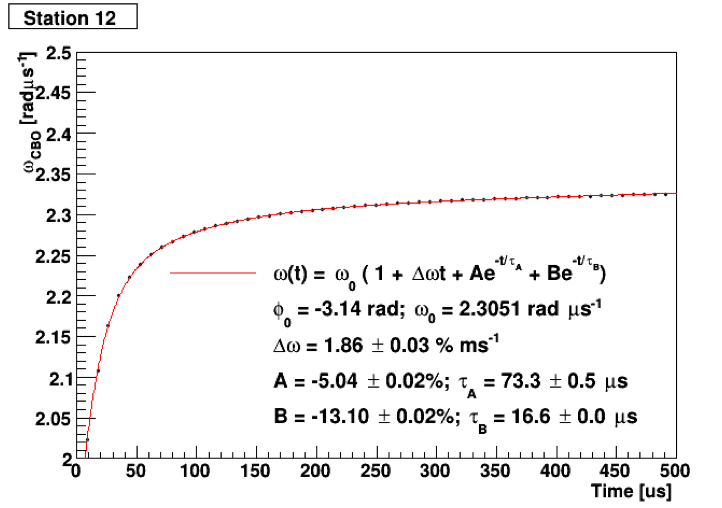
\includegraphics[width=\textwidth]{TrackerCBOModel}
	    \caption[TrackerCBOModel]{Plotted is the CBO frequency determined with tracker data as a function of time, for station 12 in the 60H dataset. The frequency was modeled as a sum of a constant with a linear part and two exponentials. It rises sharply at early times and slowly over the rest of the fill. Plot created by James Mott.}
	    \label{fig:TrackerCBOModel}
	\end{figure}


\section{Beam Dynamics: Vertical Waist Model}
\label{Sec:VW}

	\begin{enumerate}
		\item{\wa is senstive to the width of the beam, which is characterized by the frequency 
			\begin{gather}
				f_{VW} = f_{cyc} - 2f_{y}, \\
				f_{y} = f_{cbo} \sqrt{\frac{2f_{cyc}}{f_{cbo}} - 1}.
			\end{gather}}
		\item{An exponential function is assumed for the VW decoherence as in the CBO, and so the VW term is defined as
			\begin{gather}
					V(t) = 1 + A_{VW} e^{-t/\tau_{VW}} \cos(\omega_{VW}t + \phi_{VW})
			\end{gather}
		}
		\item{$\omega_{VW}$ is assumed to be a constant value even though the CBO frequency changes vs time.}
	\end{enumerate}

	In the 60H dataset $f_{VW} \approx \SI{2.3}{MHz} \approx 10 \cdot \omega_{a}$, which is an even multiple of the \gmtwo frequency. It turns out that any frequencies which are even multiples of the \gmtwo frequency largely cancel in the ratio. This is shown for the vertical waist in Figure \ref{fig:VWPlot}. This combined with the time randomization to remove the fast rotation ($f_{cyc}$) means the vertical waist does not need to be included in the ratio fit. This is justified by the lack of a vertical waist peak in the FFT of the residuals of the fit, as will be shown later.

	\begin{figure}[]
		\centering
		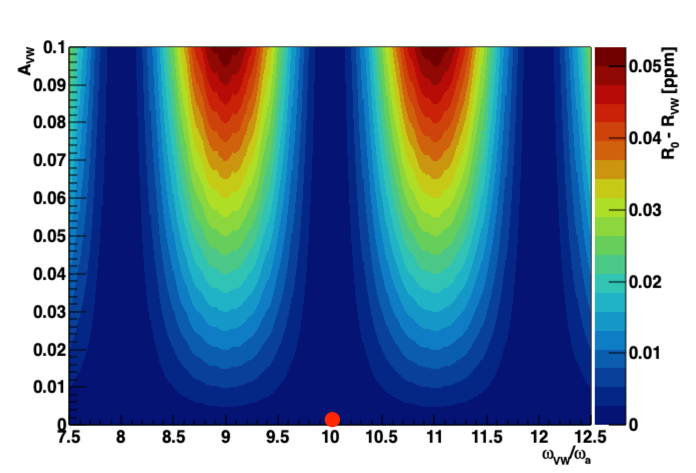
\includegraphics[width=\textwidth]{VWPlot}
	    \caption[VWPlot]{Plotted is the difference in the maximum value of the ratio with a vertical waist function included and without, as a function of both the amplitude of the vertical waist effect and the vertical waist frequency in units of the \gmtwo frequency. This was created with a toy Monte Carlo. As is shown the difference reaches a minimum for even multiples of the \gmtwo frequency. The 60H dataset lives at the bottom center of this plot, where the difference in the ratio is approximately \SI{5e-6}{} at 30 $\mu s$. Plot created by James Mott.}
	    \label{fig:VWPlot}
	\end{figure}


\section{Final Fit Function}
\label{Sec:FinalFitFunction}

	The following function is used for the final fit for each calorimeter and for the calorimeter sum:
	\begin{gather}
			R(t) = \frac{2f(t) - f_{+}(t) - f_{-}(t)}{2f(t) + f_{+}(t) + f_{-}(t)} \\[10pt]
			f_{\pm}(t) = f(t \pm T_{a}/2) \\[10pt]
			f(t) = C(t) (1 + A \cos(\omega_{a}t + \phi)) \\[10pt]
			C(t) = 1 + A_{cbo} e^{-t/\tau_{cbo}} \cos(\omega_{cbo}(t)t + \phi_{cbo}) \\[10pt]
			\omega_{a} = 2 \pi \cdot \SI{0.2291}{MHz} \cdot (1 + R \times 10^{-6})
	\end{gather}
	All parameters are floating except for terms in $\omega_{cbo}(t)$ and $\tau_{cbo}$ as described above.




\graphicspath{ {Figures/Pileup/Energies/} {Figures/Pileup/TimeSpectra/} {Figures/Main/} {Figures/ResidualsFFT/} {Figures/FitStartScans/} {Figures/FitEndScans/} {Figures/PerCalo/} }

\chapter{Analysis Results}
\label{Ch:Results}

\section{Pre-corrected and corrected energy and time spectra}

	Before fitting the data and extracting the \gmtwo frequency, pileup has to be removed. The procedure to do this was detailed in Section \ref{Sec:PileupCorrection}, and the results are shown here. Figure \ref{fig:PileupTimeSpectrum} shows the constructed pileup time spectrum, for pileup energies above threshold. The pre-corrected and corrected time spectra are not shown because differences are small and hard to see. As shown the pileup is almost completely gone by $\SI{300}{\mu s}$. The exact shape of the pileup time spectra is explained in \DB{14394}, which is in general unimportant as long as it is constructed and subtracted properly. Figure \ref{fig:ClusterEnergiesVsPileupEnergies} shows a comparison between the cluster energies and the constructed pileup energies, where differences in the two spectra are small and can be attributed to pileup contamination in the shadow method and triplets which have not been included in this analysis. Figures \ref{fig:AddedEnergies}, \ref{fig:CaloEnergies}, and \ref{fig:CaloEnergiesZoomed} show the pre-corrected and corrected energy spectra for the added histograms and for some individual calorimeters. Since the pileup energies are not perfectly reconstructed the corrected energy spectrum does not converge to 0 at the end of the high energy tail, which is readily seen in the log-scale plots. This is okay for the level of statistics included in both the 60H dataset and in Run 1. Systematic effects from getting the pileup amplitude or shape wrong are explored in Section \ref{Sec:SystematicPileup}.

	\begin{figure}[]
		\centering
		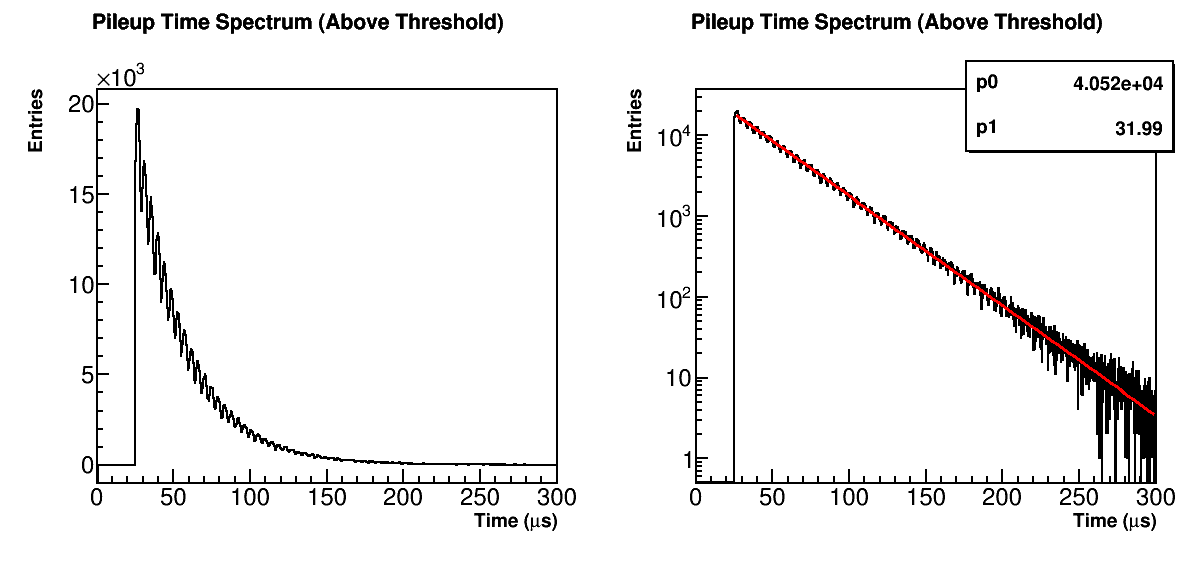
\includegraphics[width=\textwidth]{PileupTimeSpectrum}
	    \caption[PileupTimeSpectrum]{Plotted is constructed pileup time spectrum on a linear (left) and log (right) scale. The histogram on the right is fit to a simple two parameter exponential to get an idea of the lifetime of the pileup, calculated here as $\SI{32.02}{\mu s}$, which is close to half of the muon lifetime at about $\SI{64.4}{\mu s}$. Reasons for why these two values don't equal include the absence of triplets, lost muons, and an improper fitting function.}
	    \label{fig:PileupTimeSpectrum}
	\end{figure}

	\begin{figure}[]
		\centering
		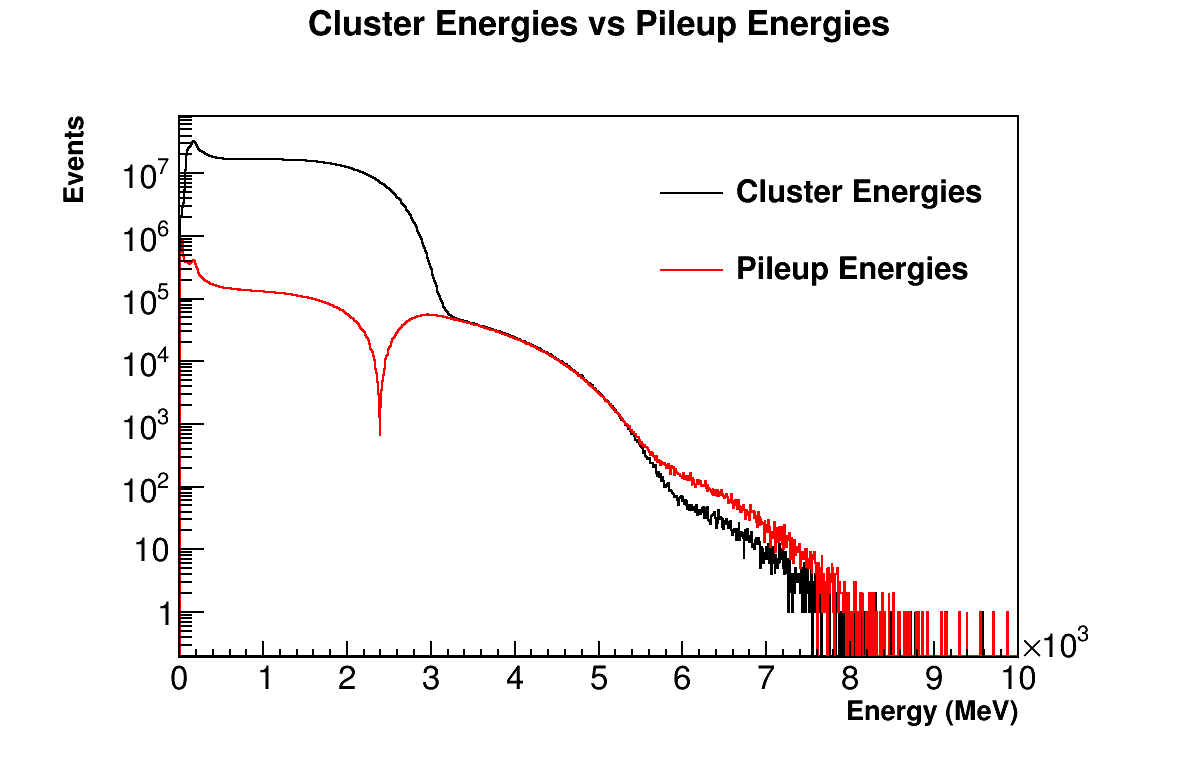
\includegraphics[width=\textwidth]{ClusterEnergiesVsPileupEnergies}
	    \caption[ClusterEnergiesVsPileupEnergies]{Cluster energies in black are plotted vs pileup energies in red, for all calorimeters added together. At energies below about 2.4 GeV the pileup spectrum goes negative. In this plot the absolute value of the pileup energies is plotted, and a spike at about 2.4 GeV can be seen as a consequence of this.}    
	    \label{fig:ClusterEnergiesVsPileupEnergies}
	\end{figure}

	\begin{figure}[]
	\centering
	    \begin{subfigure}[]{0.8\textwidth}
		    \centering
			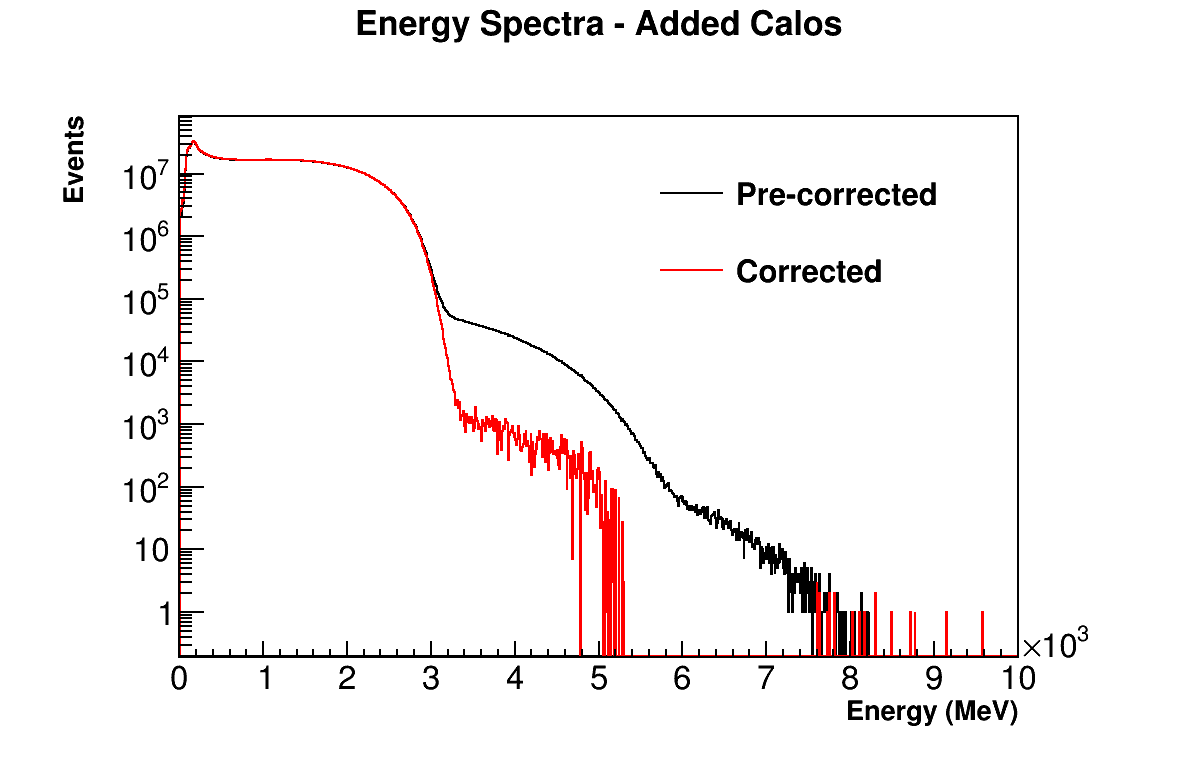
\includegraphics[width=\textwidth]{AddedEnergies}
		    \caption{Log scale - the corrected energy spectrum goes negative around 5 GeV.}
	    \end{subfigure}% %you need this % here to add spacing between subfigures
	    \vspace{1cm}
	    \begin{subfigure}[]{0.8\textwidth}
		    \centering
			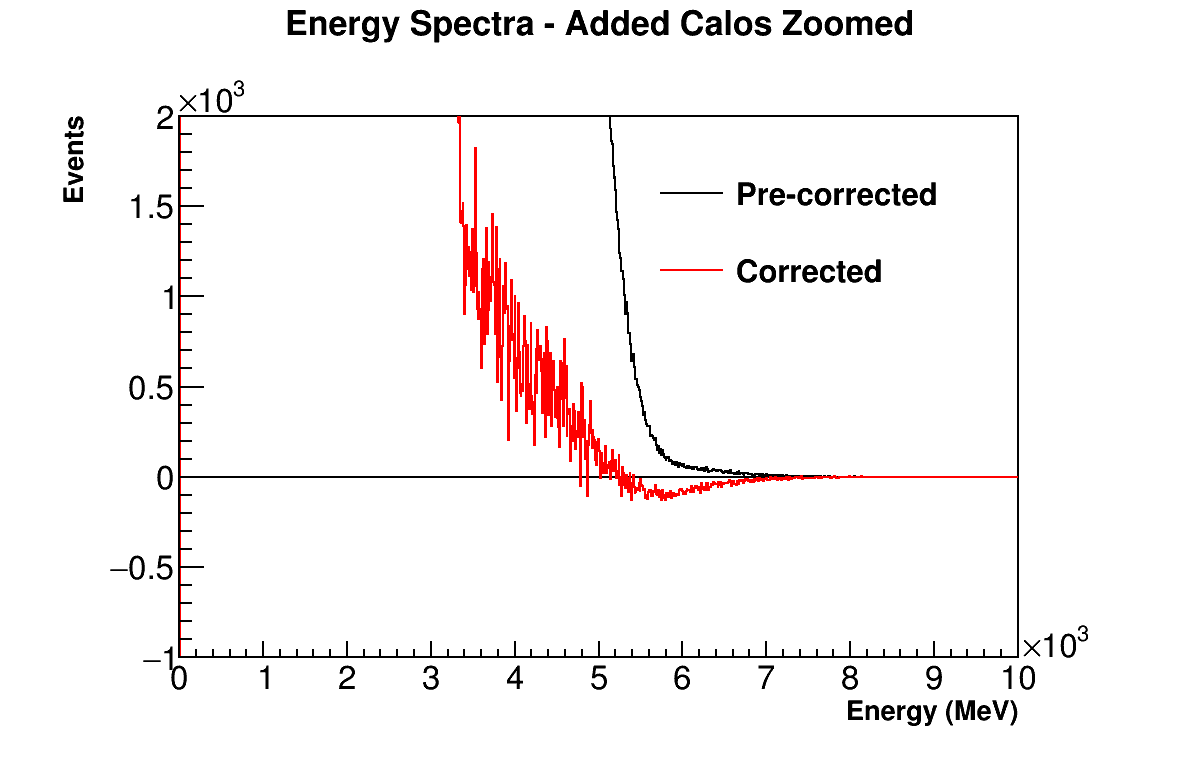
\includegraphics[width=\textwidth]{AddedEnergiesZoomed}
		    \caption{Linear scale - zoomed in to show the shape.}
	    \end{subfigure}
	\caption[AddedEnergies]{Plots for the pre-corrected and corrected energy spectra are shown, all calorimeters added together. Because the triplets and contamination are not accounted for, the corrected energy spectrum does not lie exactly along zero.}
	\label{fig:AddedEnergies}
	\end{figure}

	\begin{figure}[]
		\centering
		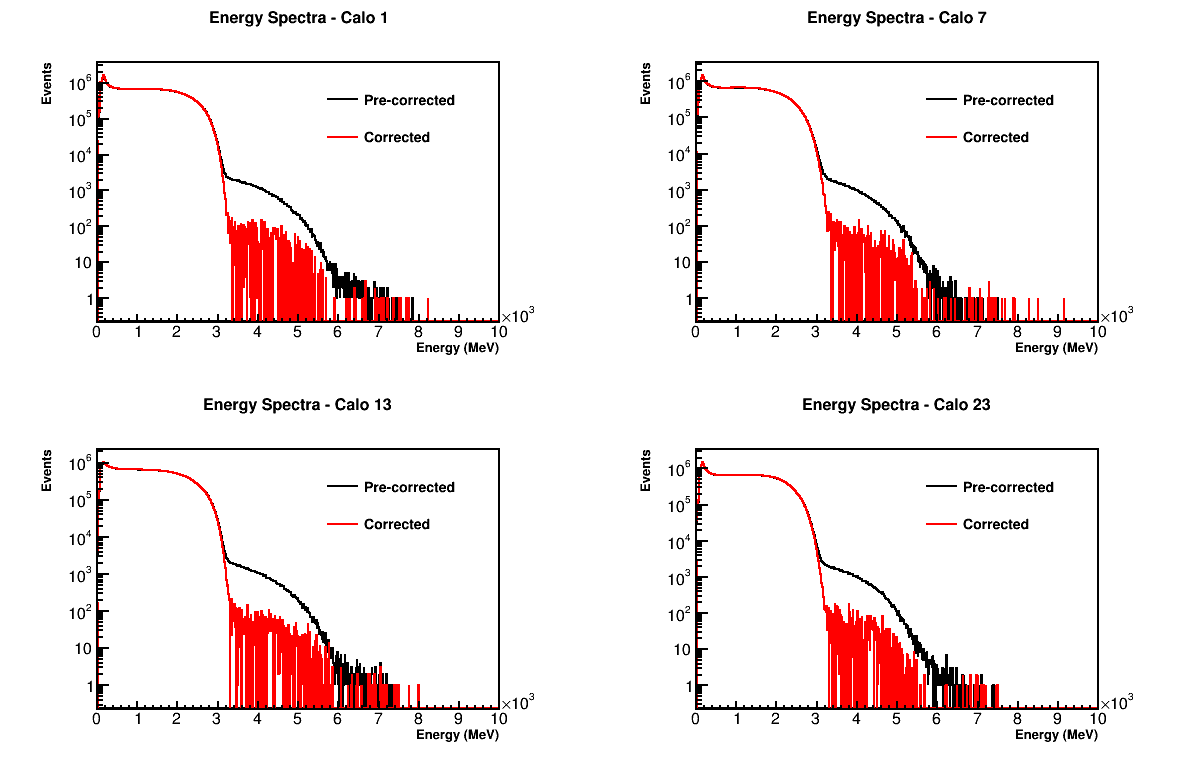
\includegraphics[width=.8\textwidth]{CaloEnergies}
	    \caption[CaloEnergies]{Pre-corrected and corrected energy spectra for calorimeters 1, 7, 13, and 23 plotted on a log scale.}    
	    \label{fig:CaloEnergies}
	\end{figure}

	\begin{figure}[]
		\centering
		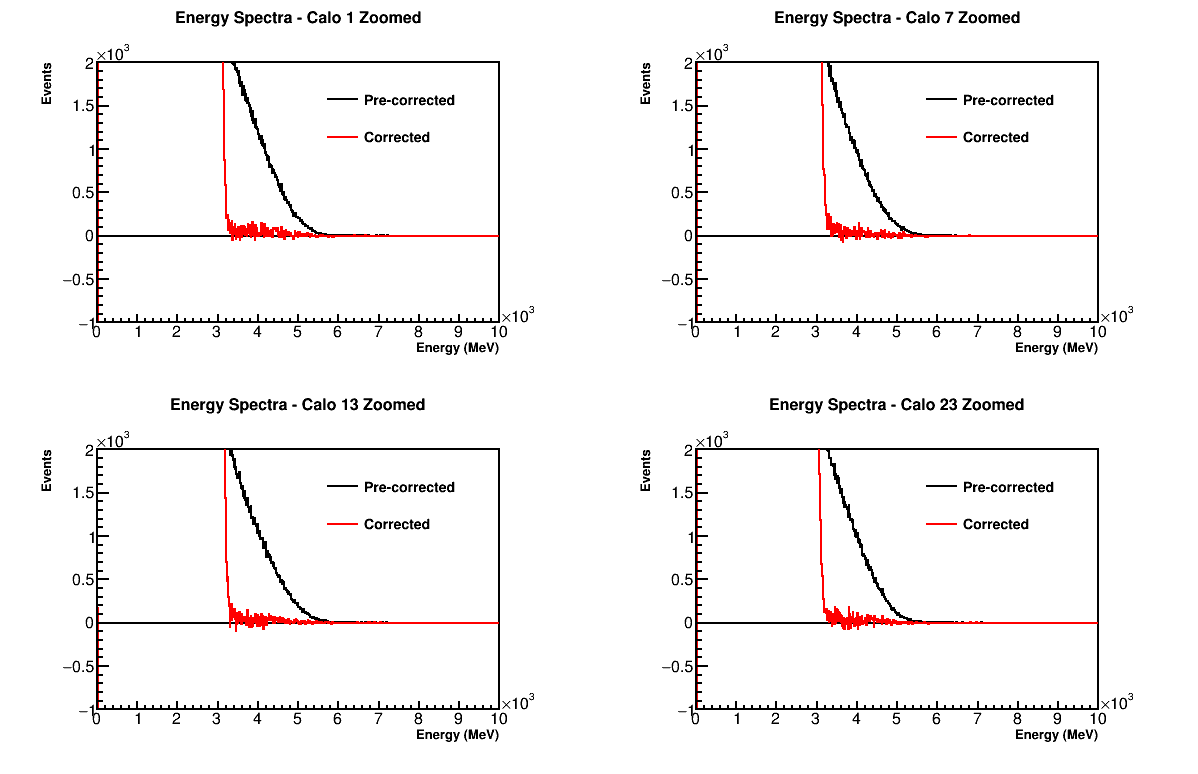
\includegraphics[width=.8\textwidth]{CaloEnergiesZoomed}
	    \caption[CaloEnergiesZoomed]{Pre-corrected and corrected energy spectra for calorimeters 1, 7, 13, and 23 plotted on a linear scale and zoomed in.}    
	    \label{fig:CaloEnergiesZoomed}
	\end{figure}

\clearpage

\section{7 Parameter Ratio Fit}

	The data has been fit to a 7 parameter function, as described in Section \ref{Sec:FinalFitFunction}, reduced from the conventional 14 parameters in a T Method fit. The results are shown in Figure \ref{fig:ratioCBO_moduloPlot}, with the fit parameters transcribed into Table \ref{Tab:FitParams}. These 7 parameters include the asymmetry ``A'', the ppm level shift in the \gmtwo frequency ``R'', the \gmtwo phase ``$\phi$'', and then 4 CBO parameters. As detailed in Section \ref{Sec:CBO}, these CBO parameters include the frequency ``$\omega_{cbo}$'', lifetime ``$\tau_{cbo}$'', and then the CBO amplitude and phase on the N term, ``$N_{cbo-A}$'' and ``$N_{cbo-\phi}$'' respectively. The CBO lifetime has been fixed in the fit to $\SI{180}{\mu s}$. The N and muon lifetime terms are unecessary because the ratio method removes those terms in the data to be fit. The ratio method also divides out slow effects, which removes the need to fit for muon losses. The lack of a low frequency rise in the FFTs of the residuals as shown in Figure \ref{fig:FFT_ratioCBOFit} justifies excluding this term. Finally, due to the specific n value used in gathering the 60H data, the vertical waist (VW) frequency just so happens to be very nearly 10 times the \gmtwo frequency. As described in Section \ref{Sec:VW} this means that the VW does not need to be included in the fit. Like the lost muons this is justified by the lack of a VW peak in the FFT of the residuals. Finally, the fit range is restricted from $\SI{30}{\mu s} - \SI{500}{\mu s}$. The early time cut is determined due the instability of the stored muon beam at early times. The late time cut was chosen to avoid the region where the ratio actually starts to widen due to low stats. (This can actually be extended beyond $\SI{500}{\mu s}$ safely but that was the limit used by default for previous datasets, and was left in when analyzing the 60H dataset. How far it should be extended is yet to be decided.)

	Table \ref{Tab:CorrMat} shows the correlation matrix for the fit parameters in the added calorimeter fit. Figure \ref{fig:CorrelationMatrix} shows the same information in graphical format. As seen the only significant correlation to R is the \gmtwo phase. This is good because it means that if other fit parameters are for some reason fitted slightly incorrectly, the resulting effect on R will be minimal.

	\begin{figure}[]
		\centering
		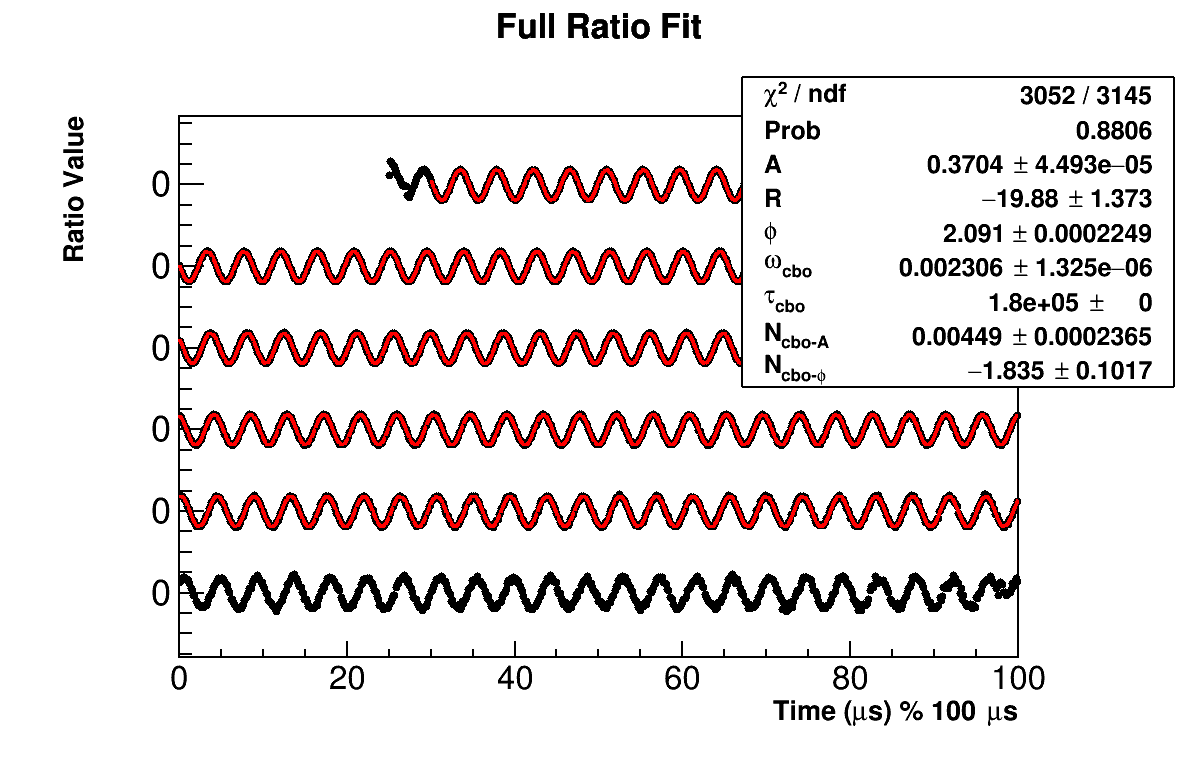
\includegraphics[width=\textwidth]{ratioCBO_moduloPlot}
	    \caption[ratioCBO_moduloPlot]{Final fit result for the 60 hour dataset. The fit includes 6 free parameters and one fixed. The x axis is in units of $\mu$s modulo 100 $\mu$s, with successive portions of the data points and fit shifted downwards on the plot. The parameter values in the stats box for the CBO frequency and lifetime are in units of ns. R is blinded locally. The fit ranges from 30 $\mu$s to 500 $\mu$s.}
	    \label{fig:ratioCBO_moduloPlot}
	\end{figure}

	\begin{table}[]
	\centering
	\setlength\tabcolsep{10pt}
	\renewcommand{\arraystretch}{1.2}
	\begin{tabular*}{.8\linewidth}{@{\extracolsep{\fill}}|l|l|c|c|}
	  \hline
	  	\multicolumn{4}{|c|}{\textbf{Fit Results}} \\
	  \hline\hline
	  	\multicolumn{2}{|c}{$\chi^{2}$/NDF}       				&  \multicolumn{2}{c|}{$3052/3145$}  \\
	  	\multicolumn{2}{|c}{P value}         	 				&  \multicolumn{2}{c|}{$0.8806$}  \\
	  \hline\hline
	  	Parameter & Descriptor & Value & Error \\
	  \hline
		$A$    			 	  & Asymmetry  	    			&  $0.3704$  	&	$\SI{4.493e-5}{}$  \\
		$R$     			  & R (ppm, blinded)   	 		&  $-19.88$  	&	$1.373$  \\
		$\phi$   			  & \gmtwo Phase         		&  $2.091$  	&	$\SI{2.249e-4}{}$  \\
		$\omega_{cbo}$   	  & CBO Frequency $(ns^{-1})$   &  $0.002306$  	&	$\SI{1.325e-6}{}$  \\
		$\tau_{cbo}$ (fixed)  & CBO Lifetime $(\mu s)$ 	    &  $180$  		&	$0$  \\
		$N_{cbo-A}$   	 	  & CBO N Amplitude      		&  $0.00449$  	&	$\SI{2.365e-4}{}$  \\
		$N_{cbo-\phi}$   	  & CBO N Phase       	 		&  $-1.835$  	&	$0.1017$  \\
	  \hline
	\end{tabular*}
	\caption{Table of final fit results.}
	\label{Tab:FitParams}
	\end{table}

	\begin{table}[]
	\setlength\tabcolsep{0pt}
	\begin{tabular*}{\linewidth}{@{\extracolsep{\fill}}lLBLLLLL}
	  \toprule
	            & \thead{$A$} & \thead{$R$} & \thead{$\phi$} & \thead{$\omega_{cbo}$} & \thead{$\tau_{cbo}$ (fixed)} & \thead{$N_{cbo-A}$} & \thead{$N_{cbo-\phi}$} \\
	  \midrule
		$A$    			 	 &  1.0000  &  0.0049  & -0.0068  & -0.0166  &  0.0000  & -0.0098  &  0.0233  \\
		$R$     			 &  0.0049  &  1.0000  & -0.8300  & -0.0204  &  0.0000  &  0.0207  &  0.0282  \\
		$\phi$   			 & -0.0068  & -0.8300  &  1.0000  &  0.0280  &  0.0000  & -0.0287  & -0.0387  \\
		$\omega_{cbo}$   	 & -0.0166  & -0.0204  &  0.0280  &  1.0000  &  0.0000  &  0.0773  & -0.8585  \\
		$\tau_{cbo}$ (fixed) &  0.0000  &  0.0000  &  0.0000  &  0.0000  &  1.0000  &  0.0000  &  0.0000  \\
		$N_{cbo-A}$   	 	 & -0.0098  &  0.0207  & -0.0287  &  0.0773  &  0.0000  &  1.0000  & -0.0656  \\
		$N_{cbo-\phi}$   	 &  0.0233  &  0.0282  & -0.0387  & -0.8585  &  0.0000  & -0.0656  &  1.0000  \\
	  \bottomrule
	\end{tabular*}
	\caption{Correlation matrix for the full ratio fit. The CBO lifetime is fixed but included in this table. The only significant correlation to R is the \gmtwo phase.}
	\label{Tab:CorrMat}
	\end{table}

	\begin{figure}[]
		\centering
		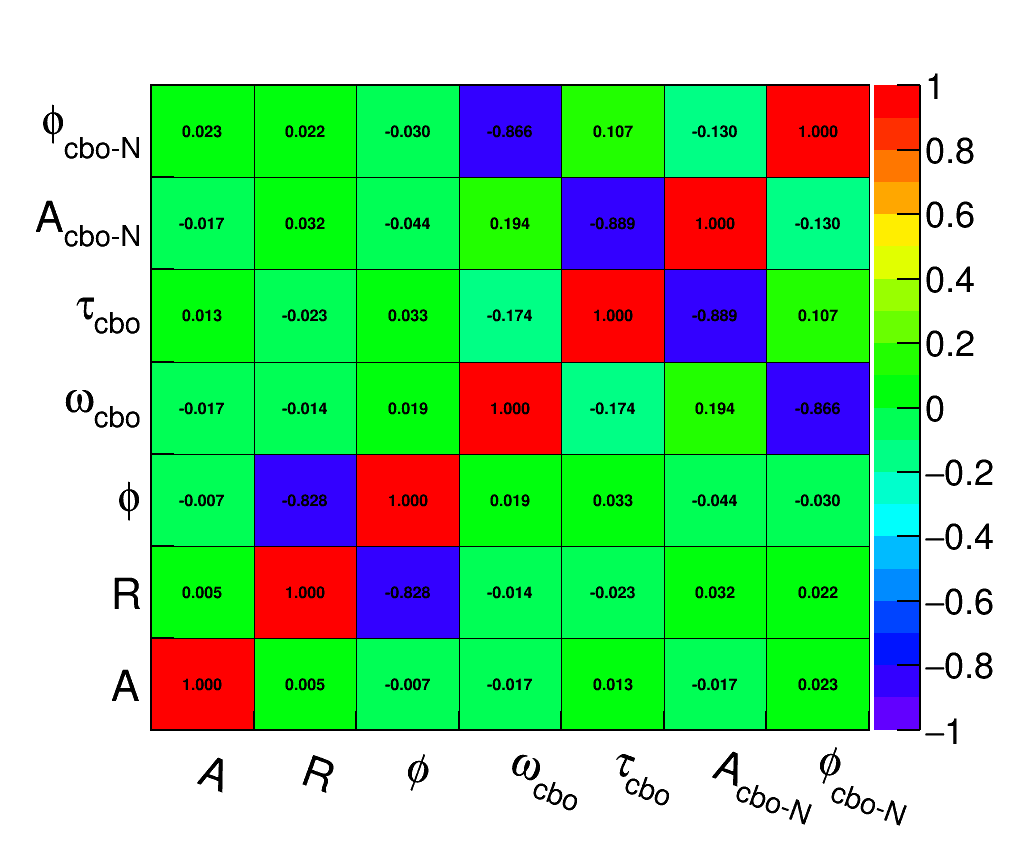
\includegraphics[width=\textwidth]{CorrelationMatrix}
	    \caption[CorrelationMatrix]{Plotted are the correlations between the different fit parameters. Correlations to R are minimal for all fit parameters except the \gmtwo phase. The correlation between the CBO frequency and phase is also easily noticed in this plot.}
	    \label{fig:CorrelationMatrix}
	\end{figure}

\clearpage

\section{Residual and FFT}

	In order to examine the goodness-of-fit, the residuals and the FFT of the residuals need to be examined. The residuals as well as the pulls are shown in Figure \ref{fig:fitResidual}. Also included is a plot of the pulls projected down onto the Y axis. In all three plots no substructure is immediately obvious, and in the latter the pull plot can be seen to have a mean consistent with 0 and an RMS consistent with 1, preliminarily indicating that the fit is good. Plotted in Figure \ref{fig:FFT_ratioCBOFit} is the FFT of the residuals. As can be seen no physical frequencies are observable above the noise. This shows that the CBO has been fitted correctly, and justifies the lack of a muon losses or vertical waist term in the fit. Figure \ref{fig:FFTComparison_RatioCBO} shows a similar plot, but this time overlayed with the FFT of the fit residuals for a 5 parameter fit. As seen the CBO, VW, \gmtwo, and their beat frequencies, as well as the lost muon peak at low frequencies are removed when performing the full ratio fit.


	\begin{figure}[h]
	\centering
	    \begin{subfigure}[]{0.45\textwidth}
		    \centering
			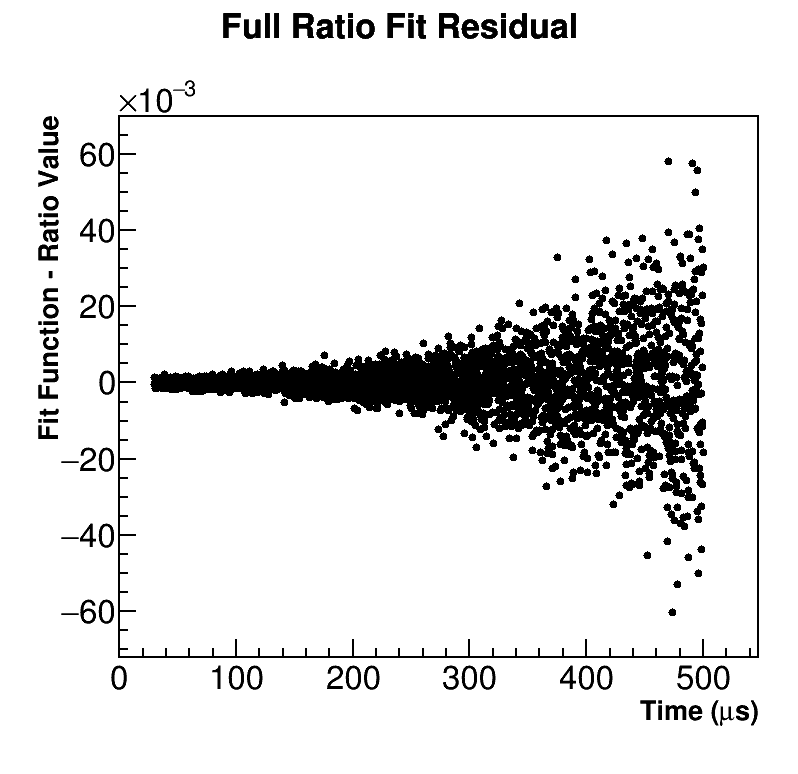
\includegraphics[width=\textwidth]{fitResidual}
		    \caption{Fit residuals.}
	    \end{subfigure}
	    \begin{subfigure}[]{0.45\textwidth}
		    \centering
			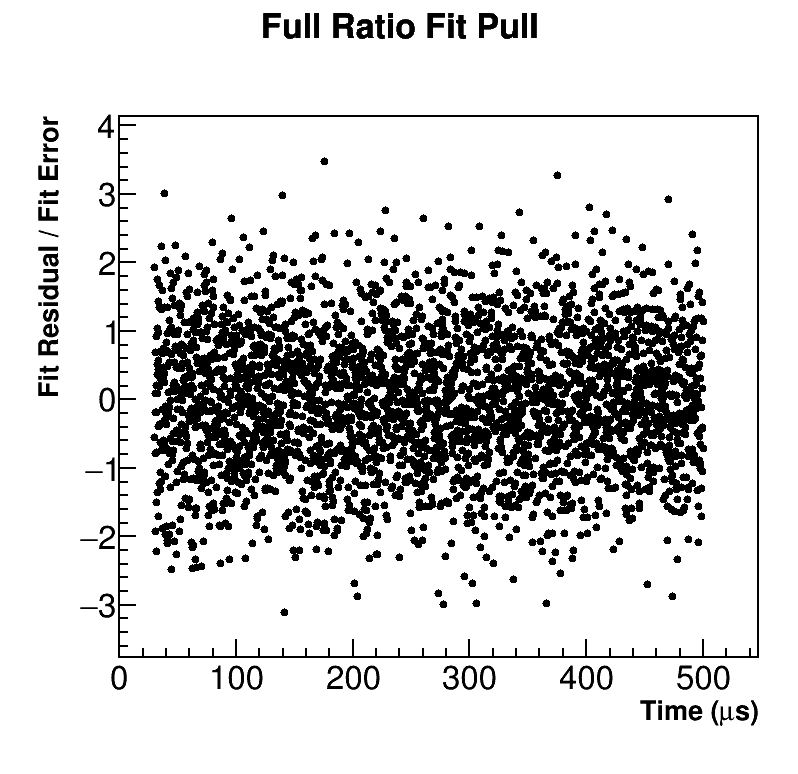
\includegraphics[width=\textwidth]{fitPull}
		    \caption{Fit pulls.}
	    \end{subfigure}% %you need this % here to add spacing between subfigures
	    \vspace{4mm}
	    \begin{subfigure}[]{0.7\textwidth}
		    \centering
			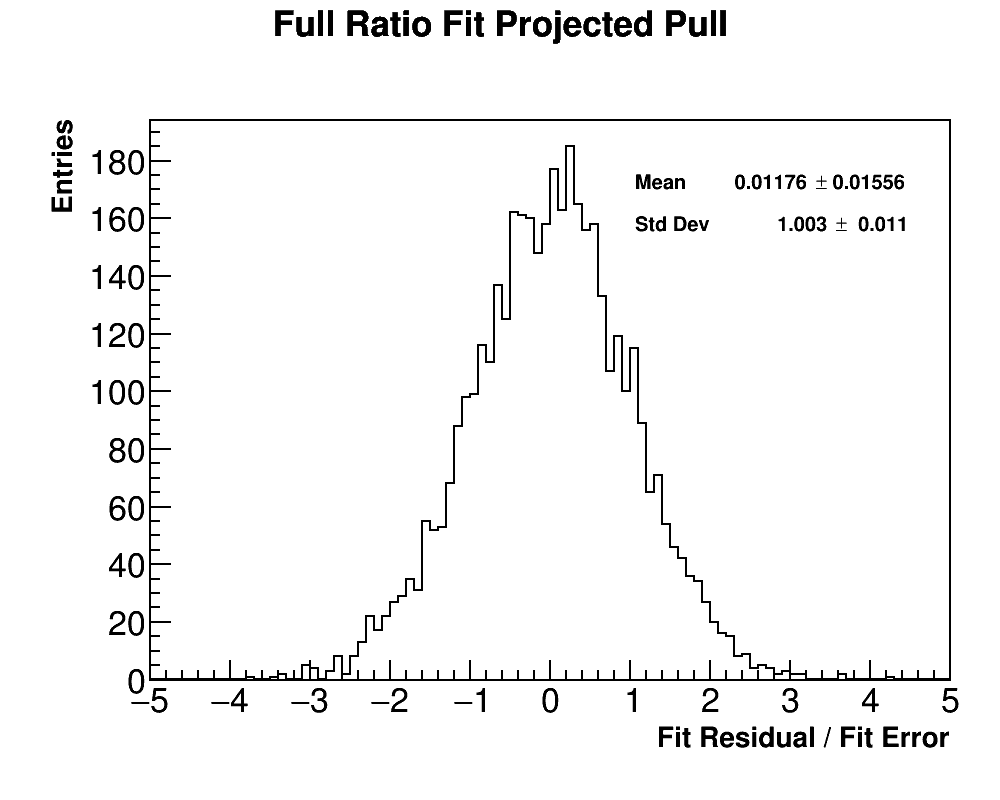
\includegraphics[width=\textwidth]{fitPull_projected}
		    \caption{Fit pulls projected onto the y axis. Note the Gaussian shape centered around 0 with unit width.}
	    \end{subfigure}
	\caption[fitResidual]{Residuals and pulls for the full ratio fit.}
	\label{fig:fitResidual}
	\end{figure}

	\begin{figure}[]
		\centering
		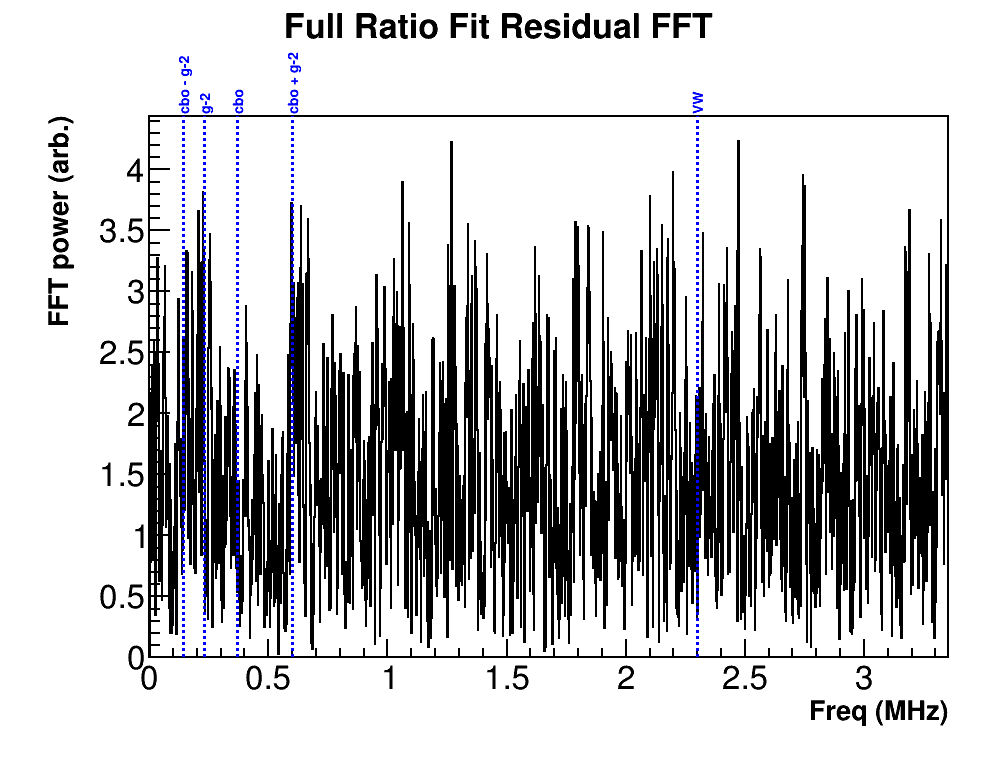
\includegraphics[width=\textwidth]{FFT_ratioCBOFit}
	    \caption[FFT_ratioCBOFit]{FFT of the residuals of the full ratio fit. No significant peaks remain in the ratio fit residuals after fitting with CBO terms. Overlayed are dotted lines for the \gmtwo, CBO, and vertical waist frequencies. Peaks close to the lines are coincidental but don't line up when zoomed in.}
	    \label{fig:FFT_ratioCBOFit}
	\end{figure}

	\begin{figure}[]
		\centering
		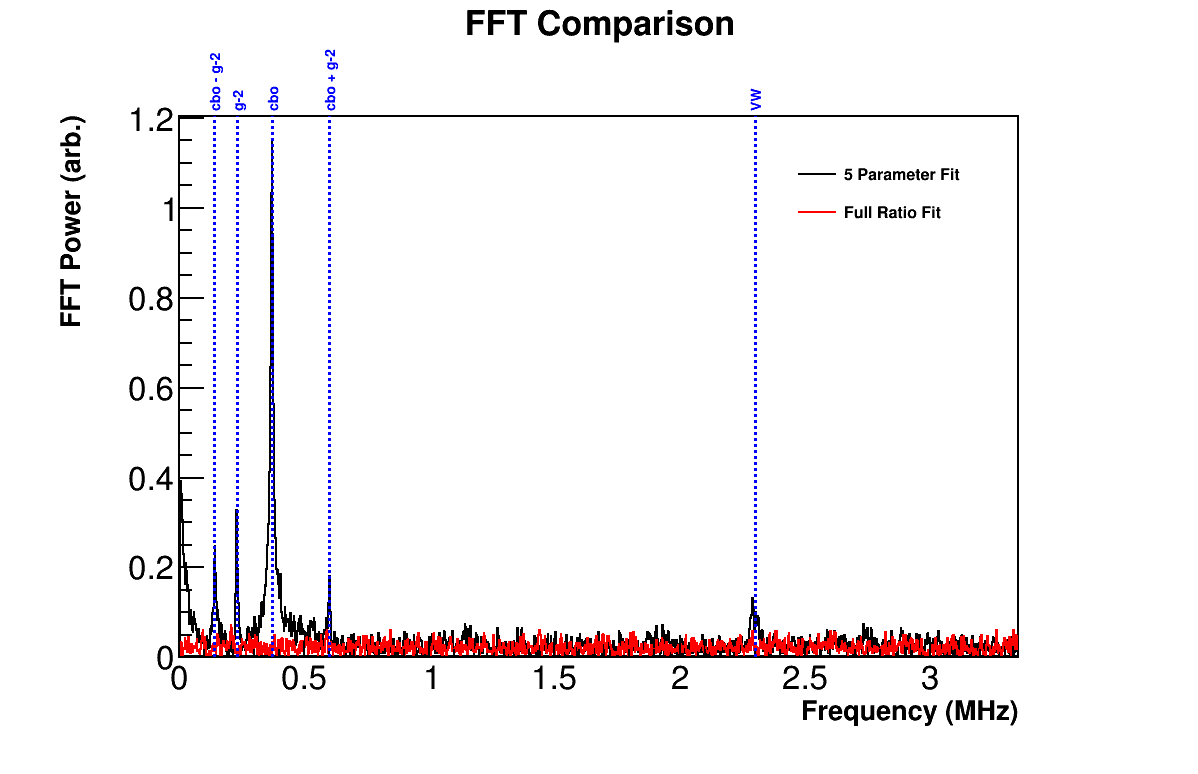
\includegraphics[width=\textwidth]{FFTComparison_RatioCBO}
	    \caption[FFTComparison_RatioCBO]{A plot of the FFT of the residuals of the fit for the five parameter fit compared to the ratio fit. In black is the FFT for a five parameter fit, where peaks for the CBO and vertical waist can be seen as well as the \gmtwo peak. In red is the FFT of the full ratio fit residuals, where it has been scaled up to be visible on this plot.}
	    \label{fig:FFTComparison_RatioCBO}
	\end{figure}

\clearpage

\section{Start time scans}

	Also necessary to determine whether the fit has been performed appropriately, is to perform start time scans. This procedure involves changing the start bound of the fit as a function of time, and making sure that fit results are consistent. If effects in the data are not properly accounted for, then fit parameters or the goodness-of-fit will change over time and will wander far outside the statistical limits defined by the reduction in data that is fitted. An example of this is shown in Section \ref{Sec:CBOFreq}, where the CBO freqency was originally modelled incorrectly. For the full ratio fit it turns out that this is the only effect that has a negative impact on the fit vs fit start time. As shown in Figure \ref{fig:Chi2FSScan} the goodness-of-fit is consistent over time, only wandering outside the statistical bands slightly. (This is also partly due to the randomization as mentioned in Section \ref{Sec:Randomization}.) Similarly Figure \ref{fig:FitStartScans} shows fit start time scans for each free parameter in the fit. All fit parameters lie comfortably within the statistical bands and are stable vs fit start time, indicating again that the fit is behaving properly.

	\begin{figure}[h]
		\centering
		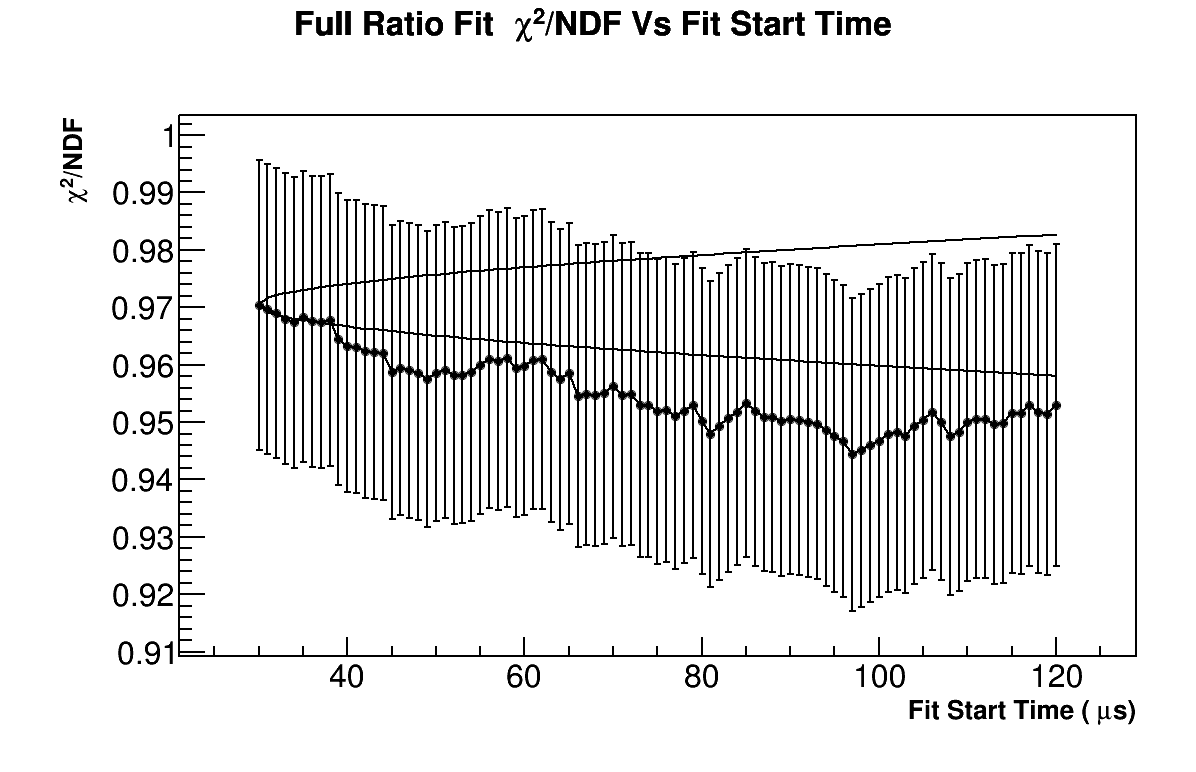
\includegraphics[width=\textwidth]{RatioCBO_Chi2NDF_Vs_FS_canv}
	    \caption[Chi2FSScan]{Plotted is the \chisq per degree of freedom vs the start time of the fit. The solid lines indicate the one sigma statistically allowed difference in the fit result coming from the reduction in the data included in the fit. The error bars on the points are calculated as $\sqrt{2/NDF}$.}
	    \label{fig:Chi2FSScan}
	\end{figure}


	\begin{figure}[]
	\centering
	    \begin{subfigure}[t]{0.45\textwidth}
		    \centering
			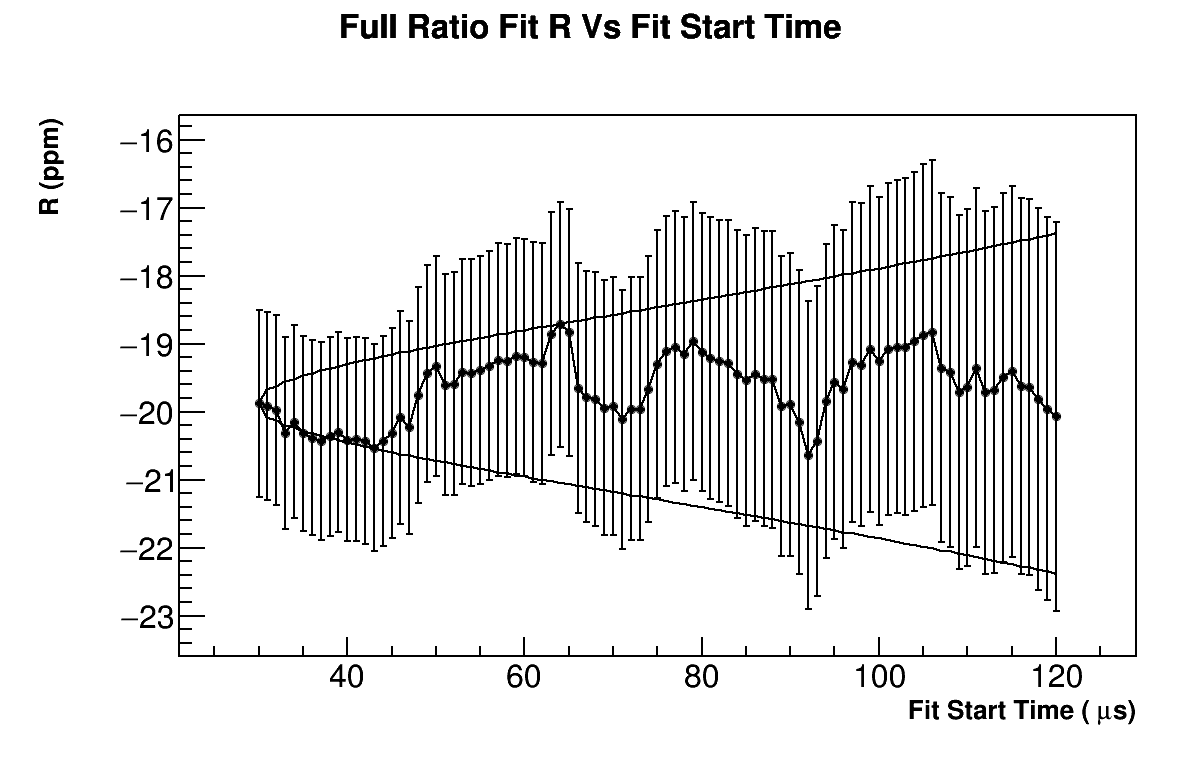
\includegraphics[width=\textwidth]{RatioCBO_R_FS_Canv}
		    \caption{Fitted R value vs fit start time.}
	    \end{subfigure}
	    \begin{subfigure}[t]{0.45\textwidth}
		    \centering
			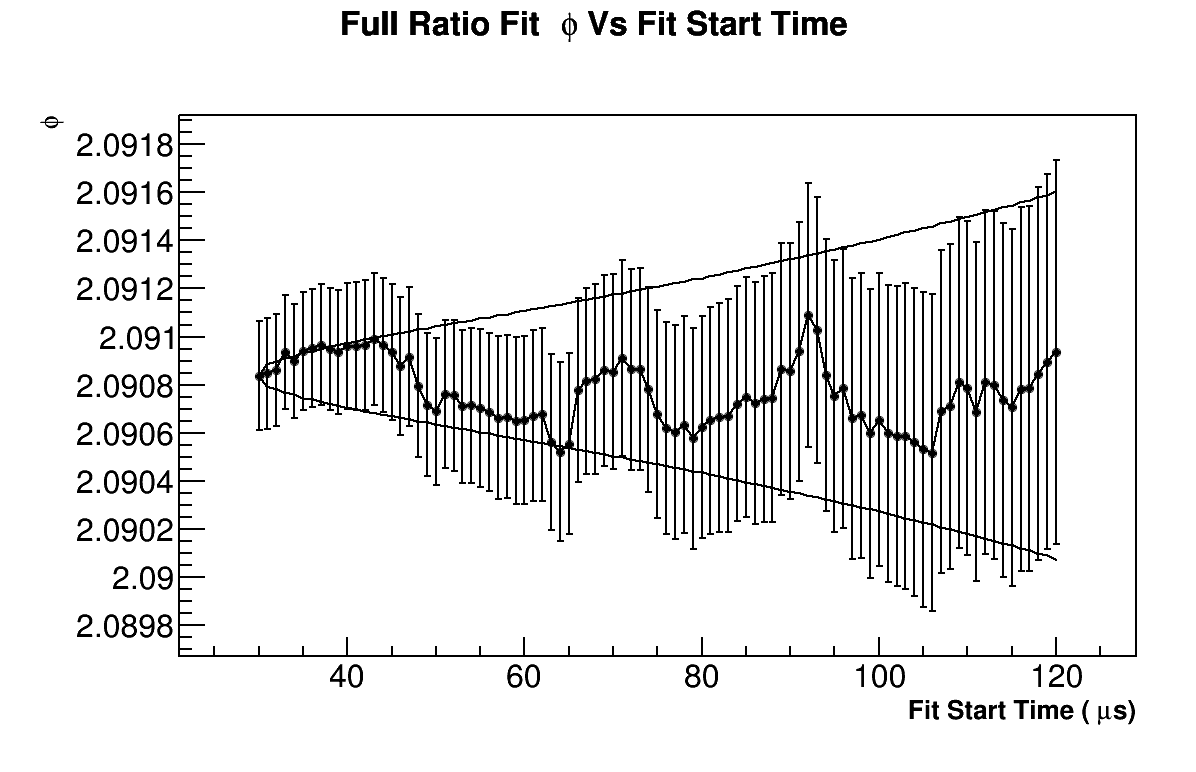
\includegraphics[width=\textwidth]{RatioCBO_phi_FS_Canv}
		    \caption{Fitted \gmtwo phase vs fit start time.}
	    \end{subfigure}% %you need this % here to add spacing between subfigures
	    \vspace{4mm}
	    \begin{subfigure}[t]{0.45\textwidth}
		    \centering
			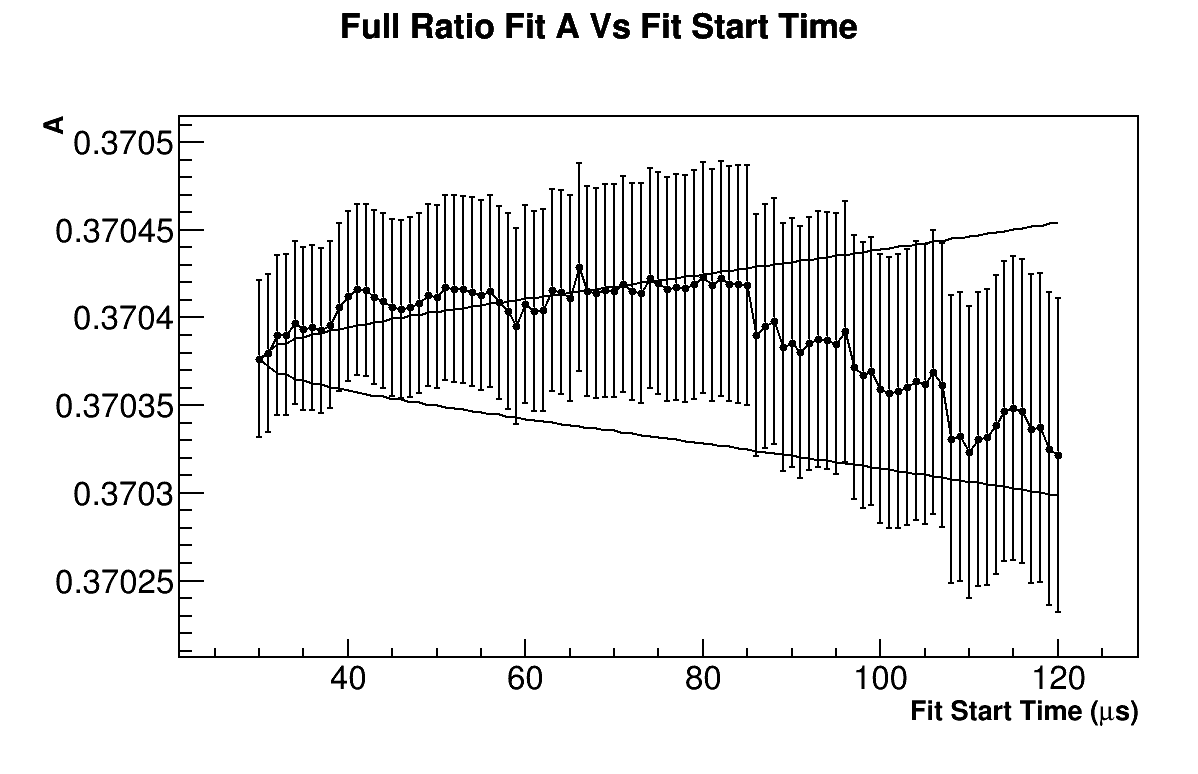
\includegraphics[width=\textwidth]{RatioCBO_A_FS_Canv}
		    \caption{Fitted asymmetry vs fit start time.}
	    \end{subfigure}
	    \begin{subfigure}[t]{0.45\textwidth}
		    \centering
			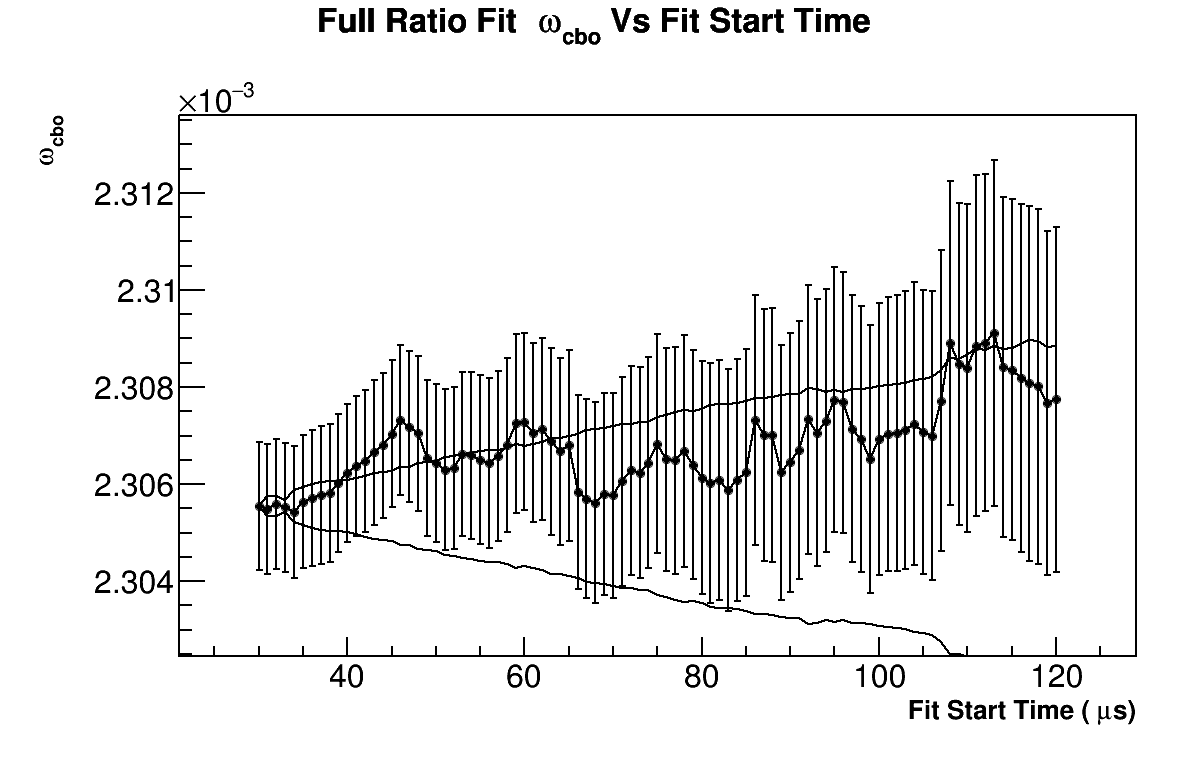
\includegraphics[width=\textwidth]{RatioCBO_omega_cbo_FS_Canv}
		    \caption{Fitted CBO frequency ($\omega_{0}$) vs fit start time.}
	    \end{subfigure}% %you need this % here to add spacing between subfigures
	    \vspace{4mm}
	    \begin{subfigure}[t]{0.45\textwidth}
		    \centering
			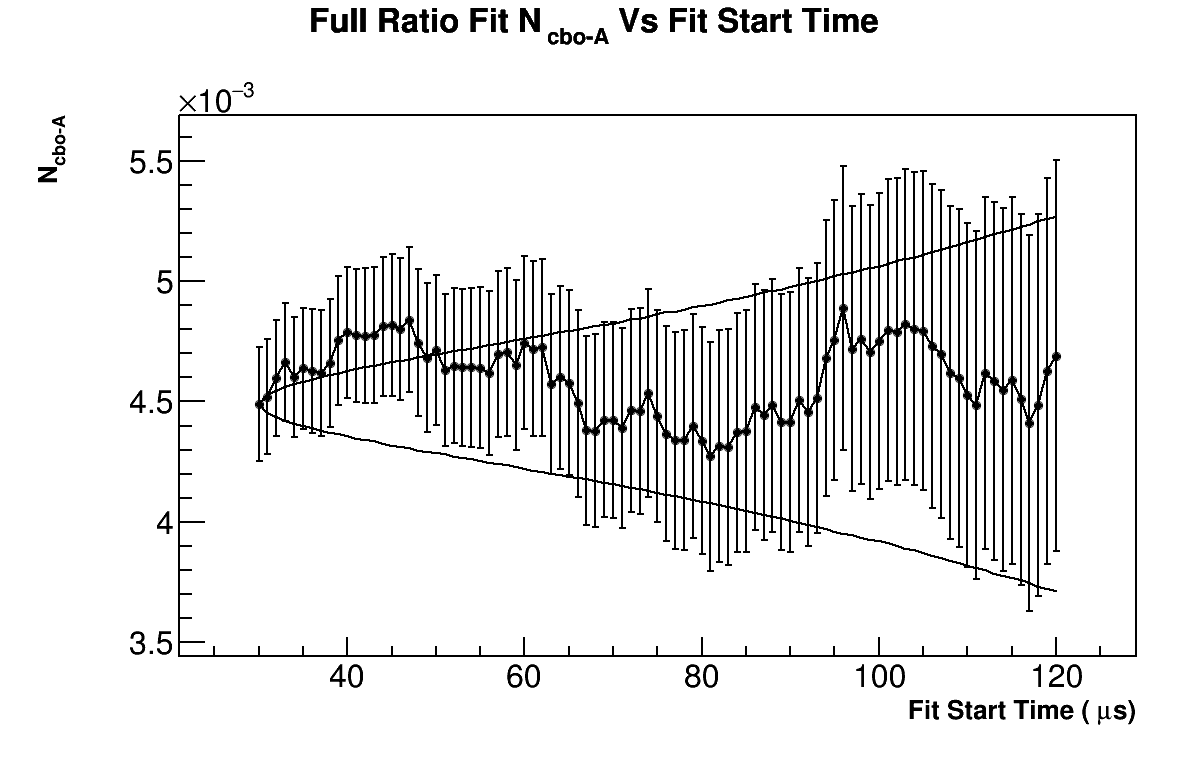
\includegraphics[width=\textwidth]{RatioCBO_N_cbo-A_FS_Canv}
		    \caption{Fitted CBO amplitdue vs fit start time.}
	    \end{subfigure}
	    \begin{subfigure}[t]{0.45\textwidth}
		    \centering
			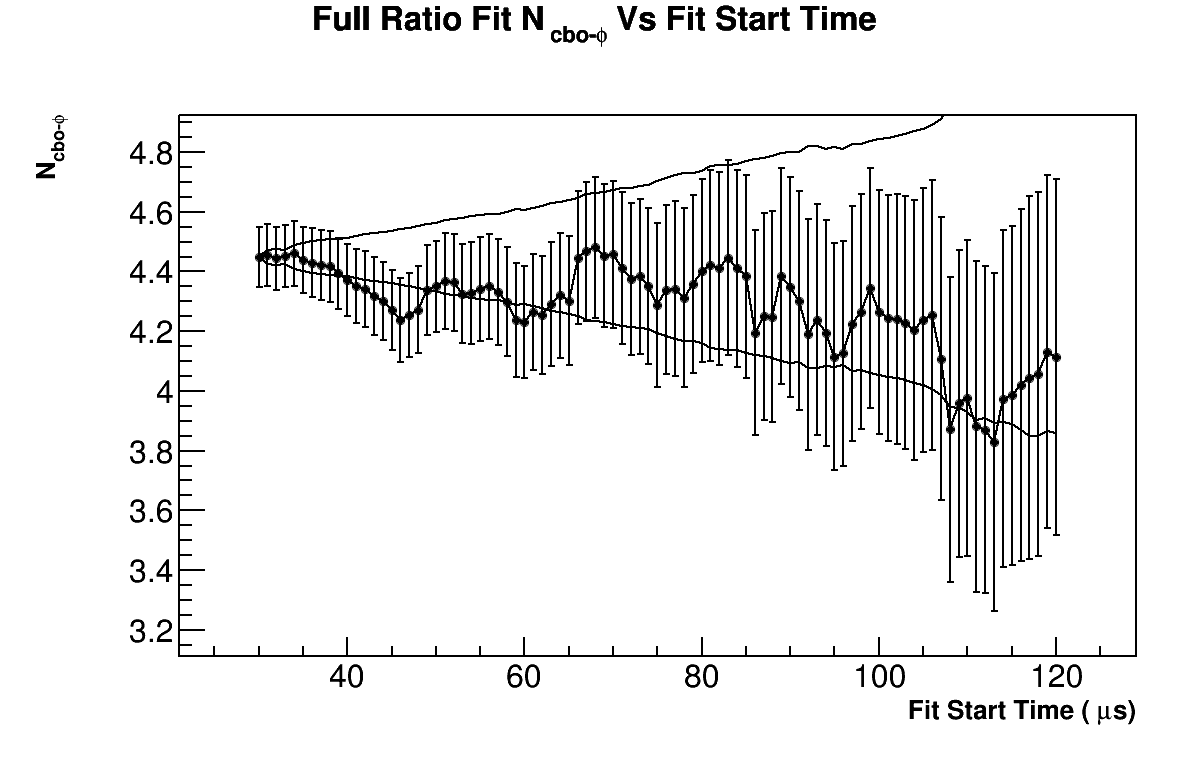
\includegraphics[width=\textwidth]{RatioCBO_N_cbo-phi_FS_Canv}
		    \caption{Fitted CBO frequency ($\omega_{0}$) vs fit start time.}
	    \end{subfigure}% %you need this % here to add spacing between subfigures
	\caption[FitStartScans]{Start time scans for the free parameters in the full ratio fit. All parameters are consistently within the one sigma statistical bands.}
	\label{fig:FitStartScans}
	\end{figure}

\clearpage

\section{End time scans}

	The uncertainties on the ratio formed from the data increase at late times as we enter regions of low stats, as shown in Figure \ref{fig:RatioLateFitEndZoomed}.  Since the ratio divides the data into 4 subsets, the time at which we enter the low stats regime can be earlier than in the standard T-method.  This is because each subset of data needs to have enough statistics such that the variation between number of entries in the subsets is unimportant and enough entries to avoid asymmetric errors when forming the ratio. It has been verified with toy MC that if the uncertainties on the ratio increase too much, then the asymmetry of the fit can be pulled, and the \chisq blows up. This can potentially lead to a poorer fit and pulling on other parameters. Performing a fit with the integral of the function as mentioned at the end of Section \ref{Sec:FinalFitFunction} mitigates this to a degree by improving the asymmetry fit parameter, but it’s still important to verify that none of the other parameters are affected in a negative way. This is simply done with fit end time scans, as shown in Figure \ref{fig:FitEndScans}. There it is seen that the goodness of fit as well as the fit parameters behave well. The asymmetry, R, and \gmtwo phase all lie comfortably within or near the statistical significance bands. These plots justify the application of a fit end time of $\SI{650}{\mu s}$ in the calorimeter sum fit.

	\begin{figure}[h]
		\centering
		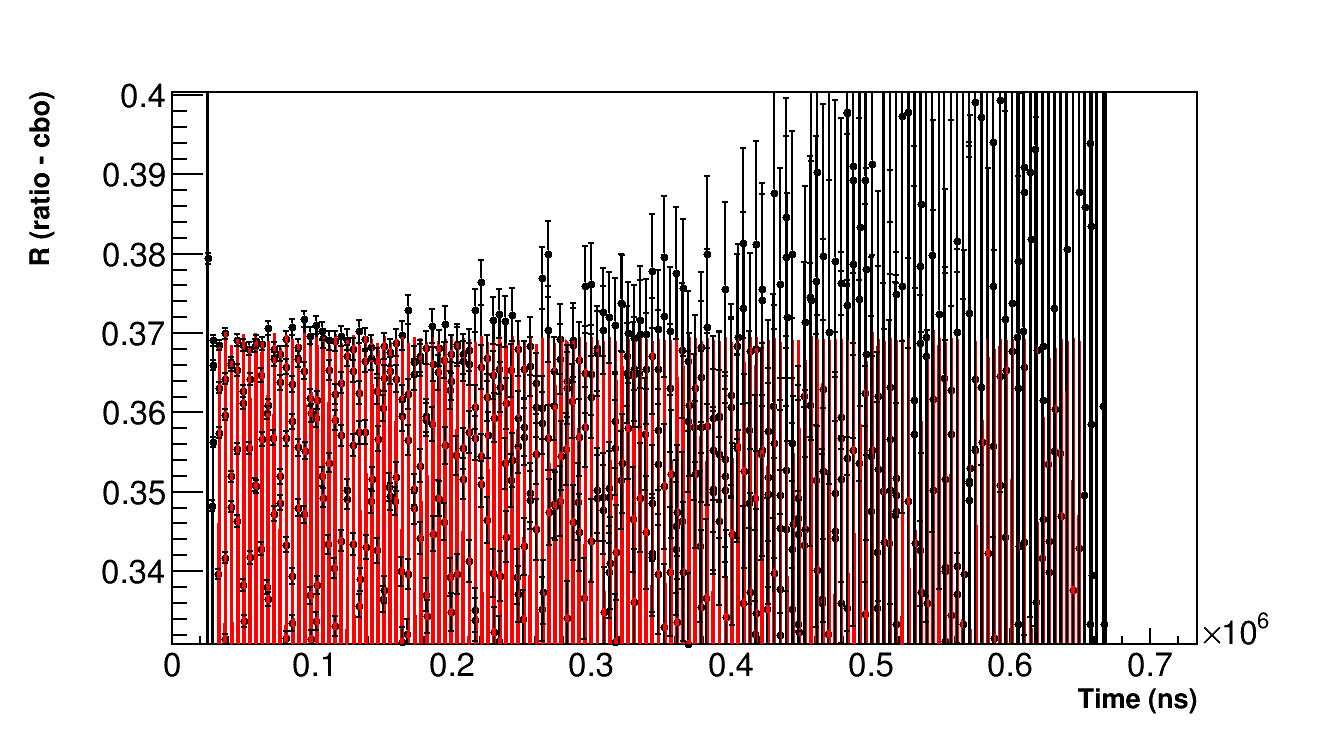
\includegraphics[width=\textwidth]{ratio-latefitend}
	    \caption[RatioLateFitEndZoomed]{The formed ratio of the data, zoomed in on the top portion. It's shown that as the time increases and the amount of data in each bin diminshes, the ratio points spread out and the errors grow large. If there is too little data, then the late times cannot be fit properly, similar to how a \chisq fit only applies to bins with enough statistics. While this effect is readily seen here, there is enough data in the 60H dataset to still be able to fit out to $\SI{650}{\mu s}$ without unduly affecting the other fit parameters.}
	    \label{fig:RatioLateFitEndZoomed}
	\end{figure}

	\begin{figure}[]
	\centering
	    \begin{subfigure}[t]{0.45\textwidth}
		    \centering
			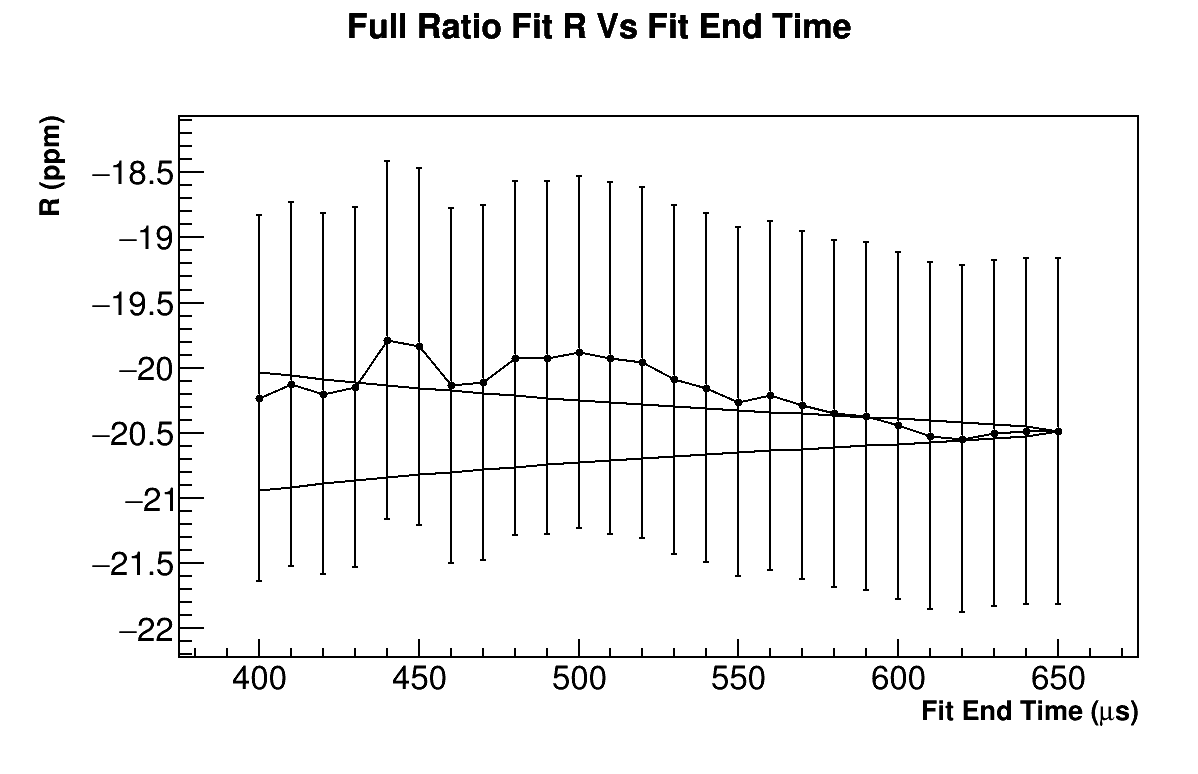
\includegraphics[width=\textwidth]{RatioCBO_R_FE_Canv}
		    \caption{Fitted R value vs fit end time.}
	    \end{subfigure}
	    \begin{subfigure}[t]{0.45\textwidth}
		    \centering
			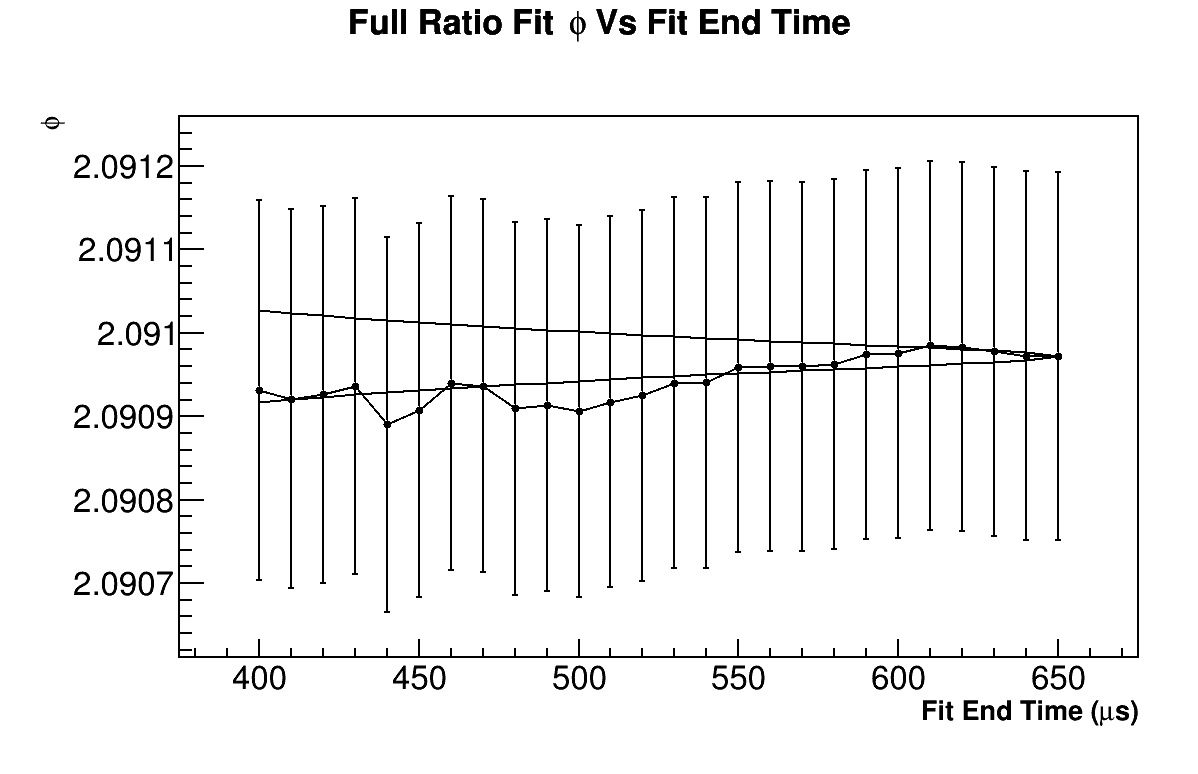
\includegraphics[width=\textwidth]{RatioCBO_phi_FE_Canv}
		    \caption{Fitted \gmtwo phase vs fit end time.}
	    \end{subfigure}% %you need this % here to add spacing between subfigures
	    \vspace{4mm}
	    \begin{subfigure}[t]{0.45\textwidth}
		    \centering
			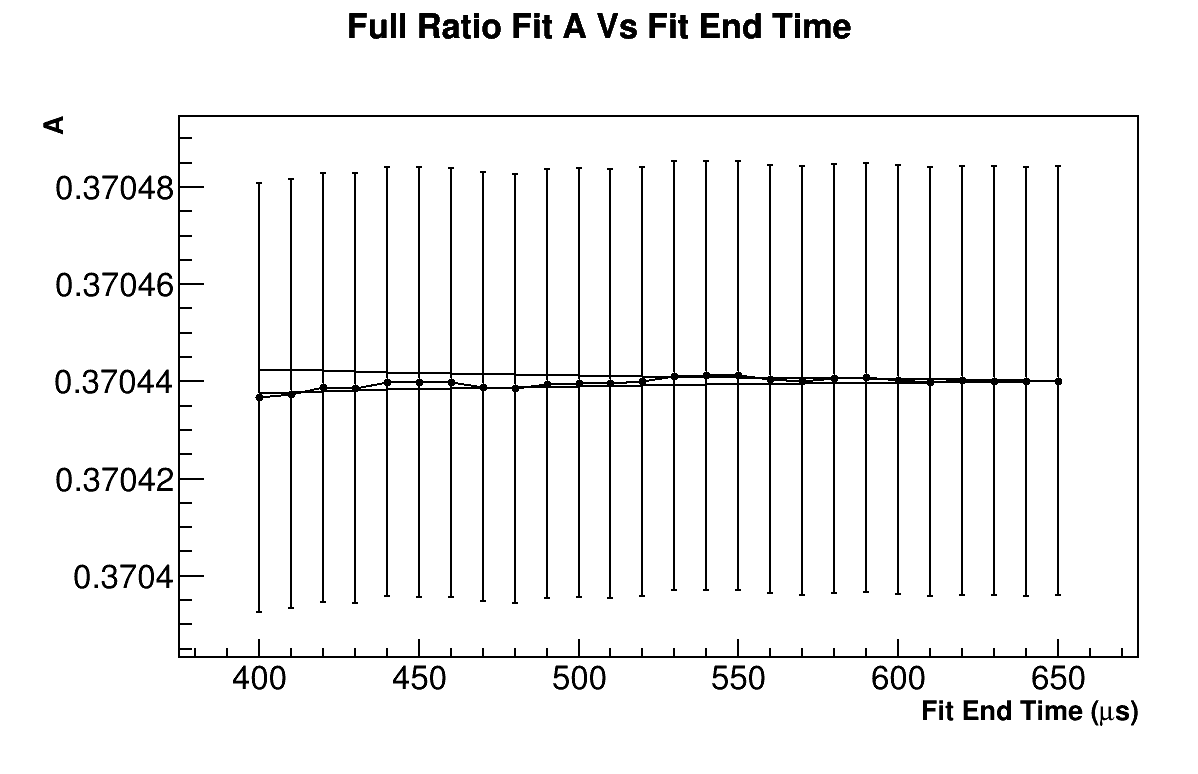
\includegraphics[width=\textwidth]{RatioCBO_A_FE_Canv}
		    \caption{Fitted asymmetry vs fit end time.}
	    \end{subfigure}
	    \begin{subfigure}[t]{0.45\textwidth}
		    \centering
			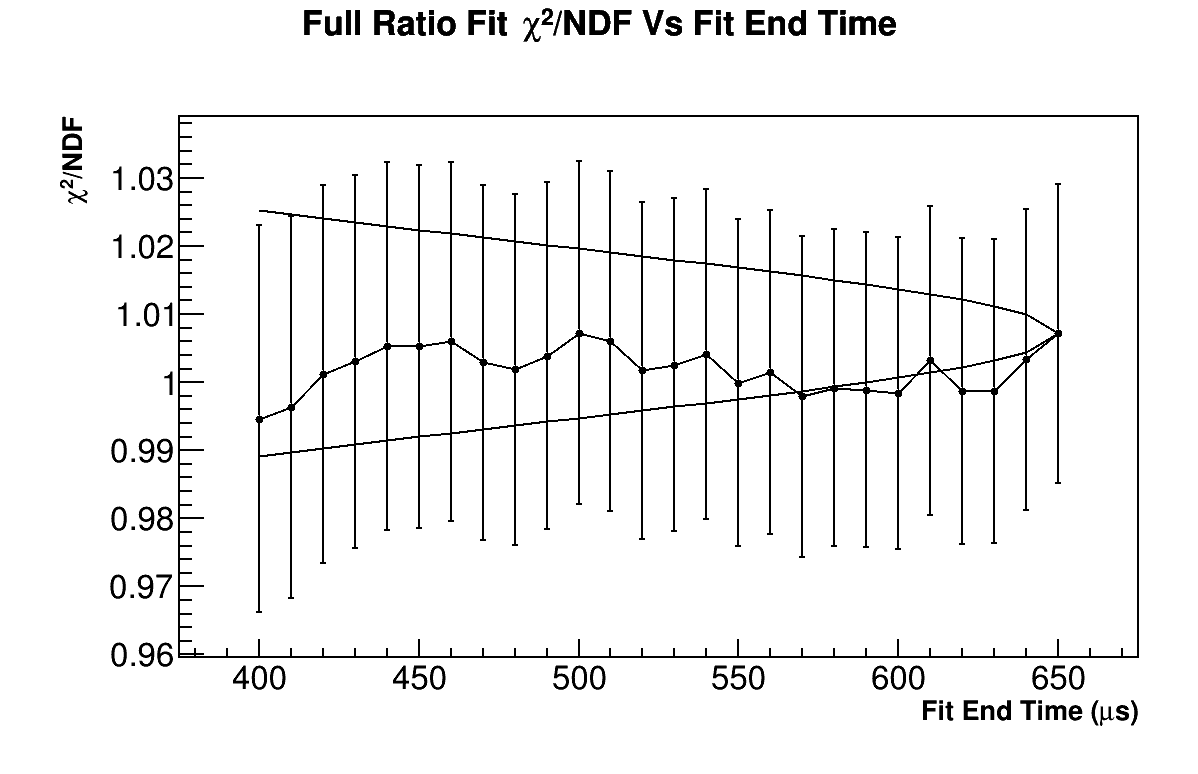
\includegraphics[width=\textwidth]{RatioCBO_Chi2NDF_Vs_FE_canv}
		    \caption{\chisq per degree of freedom vs fit end time.}
	    \end{subfigure}% %you need this % here to add spacing between subfigures
	\caption[FitEndScans]{Fit end time scans for the main free parameters in the full ratio fit, as well as the $\chi^{2}$/NDF. The statistical signifcance bands are narrow due to the small amount of data differences between successive points. The paramaters can be seen to behave well, and are not affected by the late fit end times.}
	\label{fig:FitEndScans}
	\end{figure}


\clearpage

\section{Results vs calorimeter}

	Finally results are examined on a per calorimeter basis. While there will be some differences in fit results due to the differing acceptance between the calorimeters, in general the results should be consistent. Because of the reduced amount of stats for the individual calorimeters, the fit range has been restricted to 30 - 300 $\mu s$ as opposed to 30 - 500 $\mu s$ for the added calorimeter fit. As described briefly in Section \ref{Sec:CBO}, extra CBO terms are included in the fits, including $N_{2cbo}$, $A_{cbo}$, and $\phi_{cbo}$. While not all individual calorimeters need all of these terms for good fits, some have poor \chisq's without them, as shown in Figure \ref{fig:CaloChi2s}. The fitted parameter results for individual calorimeters are shown in Figures \ref{fig:PerCaloPlots} and \ref{fig:PerCaloPlotsExtraCBOParams}, where the latter shows fit convergence for the extra CBO parameters. In only a few calorimeters are the extra CBO parameters potentially omittable, as evidenced by larger error bars on the fitted parameters. As seen all calorimeter fits and their parameters behave well.

	Of interest to note, calorimeters 13 and 19 have their \gmtwo phases converge to values similar to each other and separate from the rest of the calorimeters, as shown in Figure \ref{subfig:CaloGM2Phase}. There is also potentially a slight bump between calorimeters 1 and 24. This behaviour is matched by high $N_{cbo}$ amplitudes shown in Figure \ref{subfig:CaloNcboAmp}, and bumps in the $N_{cbo}$ phase shown in Figure \ref{subfig:CaloNcboPhase} at the same locations. These calorimeters lie behind the two tracker stations, as well as the empty tracker station near calorimeters 1 and 24. Presumably the different amount of material upstream of these calorimeters leads to a different acceptance and subsequent CBO parameters, which tie into the \gmtwo phase. It's good to see that the fitted R values for these calorimeters are not significantly different in any way. It would be interesting to see if the behaviour of these fitted parameters is reflected in simulation.

	\begin{figure}[]
	\centering
	    \begin{subfigure}[t]{0.45\textwidth}
		    \centering
			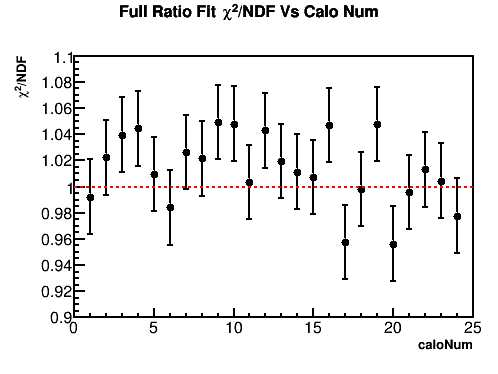
\includegraphics[width=\textwidth]{PoorCaloFits}
		    \caption{No extra CBO terms, note how most values lie above 1.}
	    \end{subfigure}
	    \hspace{4mm}
	    \begin{subfigure}[t]{0.45\textwidth}
		    \centering
			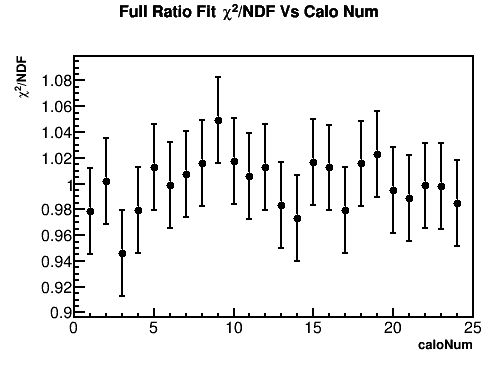
\includegraphics[width=\textwidth]{RatioCBOFit_Chi2NDF_Vs_Calo_Canv}
		    \caption{Including the extra CBO terms, the results are more or less centered around 1.}
	    \end{subfigure}
	\caption[CaloChi2s]{Plotted is the \chisq per degree of freedom vs calorimeter number. On the left are the fit results without the extra CBO terms, and on the right are the fit results with them.}
	\label{fig:CaloChi2s}
	\end{figure}


	\begin{figure}[h]
	\centering
	    \begin{subfigure}[t]{0.4\textwidth}
		    \centering
			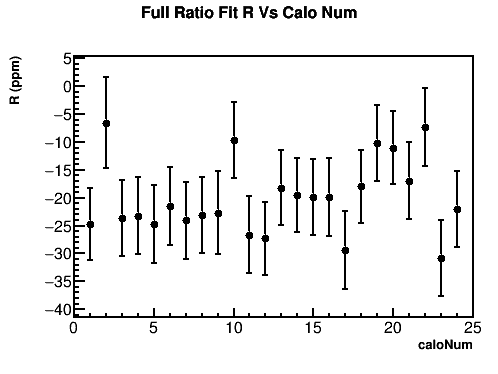
\includegraphics[width=\textwidth]{RatioCBOFit_R_Vs_Calo_Canv}
		    \caption{Fitted R value vs calorimeter number.}
	    \end{subfigure}
	    \hspace{4mm}
	    \begin{subfigure}[t]{0.4\textwidth}
		    \centering
			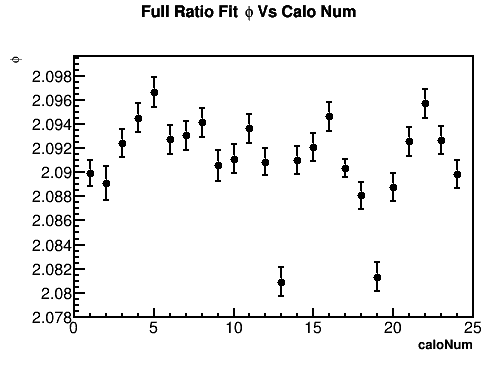
\includegraphics[width=\textwidth]{RatioCBOFit_phi_Vs_Calo_Canv}
		    \caption{Fitted \gmtwo phase vs calorimeter number. Calorimeters 13 and 19 lie behind the trackers.}
		\label{subfig:CaloGM2Phase}
	    \end{subfigure}% %you need this % here to add spacing between subfigures
	    \vspace{4mm}
	    \begin{subfigure}[t]{0.4\textwidth}
		    \centering
			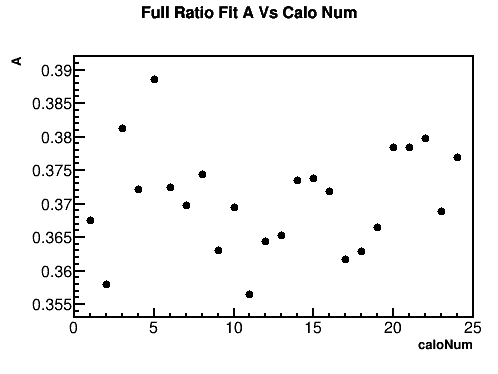
\includegraphics[width=\textwidth]{RatioCBOFit_A_Vs_Calo_Canv}
		    \caption{Fitted asymmetry vs calorimeter number.}
	    \end{subfigure}
	    \hspace{4mm}
	    \begin{subfigure}[t]{0.4\textwidth}
		    \centering
			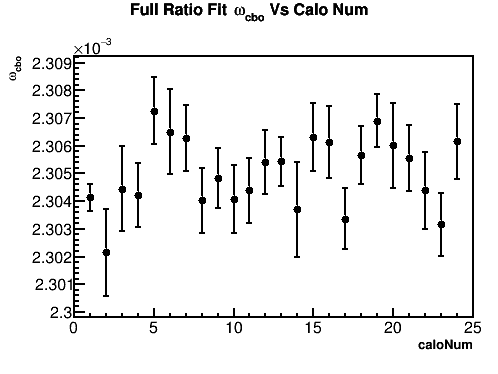
\includegraphics[width=\textwidth]{RatioCBOFit_omega_cbo_Vs_Calo_Canv}
		    \caption{Fitted CBO frequency ($\omega_{0}$) vs calorimeter number.}
	    \end{subfigure}% %you need this % here to add spacing between subfigures
	    \vspace{4mm}
	    \begin{subfigure}[t]{0.4\textwidth}
		    \centering
			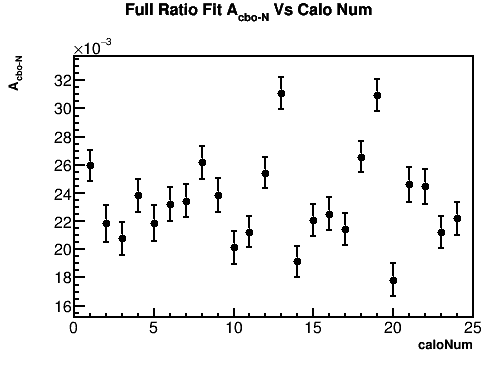
\includegraphics[width=\textwidth]{RatioCBOFit_A_cbo-N_Vs_Calo_Canv}
		    \caption{Fitted CBO amplitdue on the N parameter vs calorimeter number.}
		\label{subfig:CaloNcboAmp}
	    \end{subfigure}
	    \hspace{4mm}
	    \begin{subfigure}[t]{0.4\textwidth}
		    \centering
			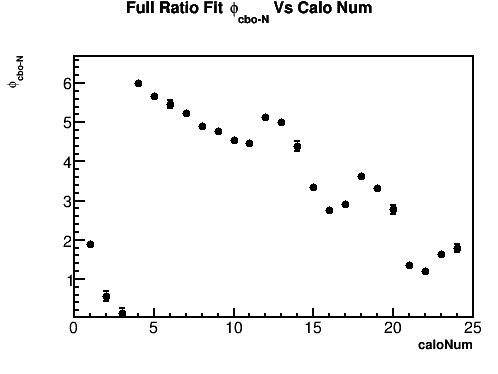
\includegraphics[width=\textwidth]{RatioCBOFit_phi_cbo-N_Vs_Calo_Canv}
		    \caption{Fitted CBO phase on the N parameter vs calorimeter number. The CBO phase varies from 0 to 2$\pi$ around the ring.}
		\label{subfig:CaloNcboPhase}
	    \end{subfigure}% %you need this % here to add spacing between subfigures
	\caption[PerCaloPlots]{Full ratio fit parameter values vs calorimeter number.}
	\label{fig:PerCaloPlots}
	\end{figure}


	\begin{figure}[h]
	\centering
	    \begin{subfigure}[t]{0.4\textwidth}
		    \centering
			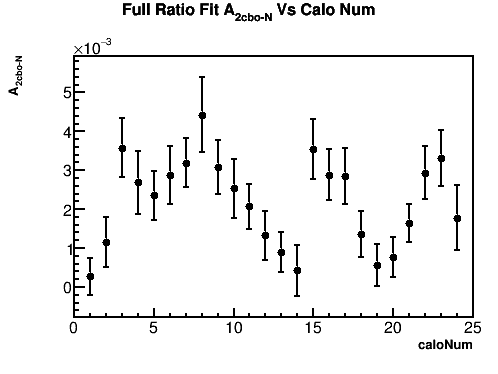
\includegraphics[width=\textwidth]{RatioCBOFit_A_2cbo-N_Vs_Calo_Canv}
		    \caption{Fitted CBO amplitdue on the N parameter for twice the CBO frequency vs calorimeter number.}
	    \end{subfigure}
	    \hspace{4mm}
	    \begin{subfigure}[t]{0.4\textwidth}
		    \centering
			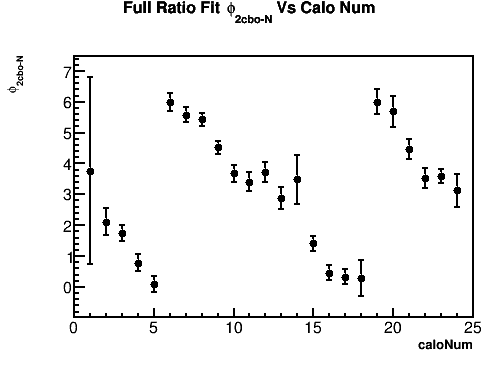
\includegraphics[width=\textwidth]{RatioCBOFit_phi_2cbo-N_Vs_Calo_Canv}
		    \caption{Fitted CBO phase on the N parameter for twice the CBO frequency vs calorimeter number.}
	    \end{subfigure}% %you need this % here to add spacing between subfigures
	    \vspace{4mm}
	    \begin{subfigure}[t]{0.4\textwidth}
		    \centering
			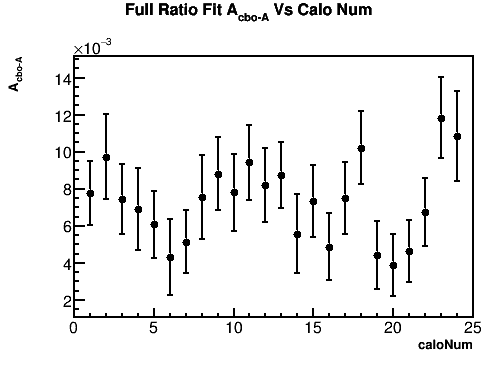
\includegraphics[width=\textwidth]{RatioCBOFit_A_cbo-A_Vs_Calo_Canv}
		    \caption{Fitted CBO amplitdue on the A parameter vs calorimeter number.}
	    \end{subfigure}
	    \hspace{4mm}
	    \begin{subfigure}[t]{0.4\textwidth}
		    \centering
			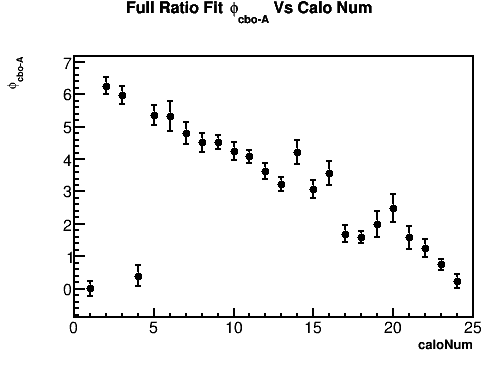
\includegraphics[width=\textwidth]{RatioCBOFit_phi_cbo-A_Vs_Calo_Canv}
		    \caption{Fitted CBO phase on the A parameter vs calorimeter number.}
	    \end{subfigure}% %you need this % here to add spacing between subfigures
	    \vspace{4mm}
	    \begin{subfigure}[t]{0.4\textwidth}
		    \centering
			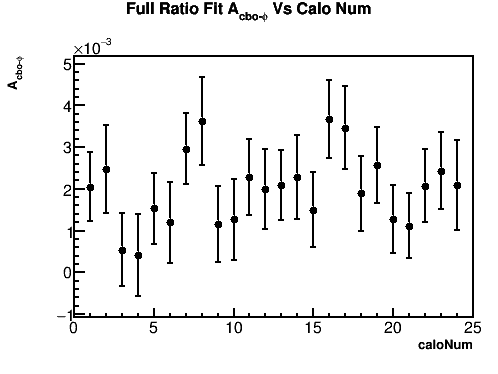
\includegraphics[width=\textwidth]{RatioCBOFit_A_cbo-phi_Vs_Calo_Canv}
		    \caption{Fitted CBO amplitdue on the \gmtwo phase parameter vs calorimeter number.}
	    \end{subfigure}
	    \hspace{4mm}
	    \begin{subfigure}[t]{0.4\textwidth}
		    \centering
			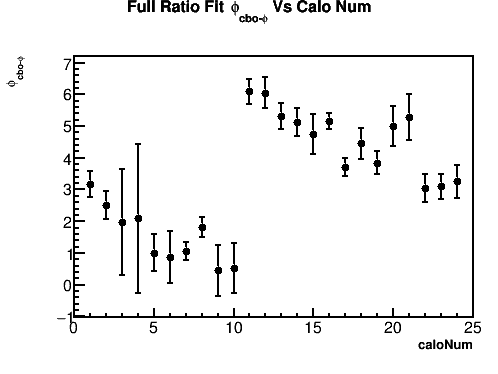
\includegraphics[width=\textwidth]{RatioCBOFit_phi_cbo-phi_Vs_Calo_Canv}
		    \caption{Fitted CBO phase on the \gmtwo phase parameter vs calorimeter number.}
	    \end{subfigure}% %you need this % here to add spacing between subfigures
	\caption[PerCaloPlotsExtraCBOParams]{Full ratio fit parameter values vs calorimeter number. Plotted here are the extra CBO parameters which improve most single calorimeter fits. In each CBO phase parameter, the phase varies from 0 to 2$\pi$ around the ring, except for the $N_{2cbo}$ term where it wraps around twice.}
	\label{fig:PerCaloPlotsExtraCBOParams}
	\end{figure}


\graphicspath{ {Figures/Pileup/Multiplier/} {Figures/Pileup/Phase/} {Figures/Pileup/EnergyScaling/} {Figures/RandomSeeds/FitStartScans/} {Figures/RandomSeeds/FitIterations/} {Figures/Miscellaneous/} {Figures/FitStartScans/} {Figures/CBO/Frequency/} {Figures/CBO/Shape/} {Figures/CBO/LifetimeScan/} {Figures/Gain/InFill/} {Figures/Gain/InFillCrystals/} {Figures/VW/} {Figures/LostMuons/} {Figures/BunchNumber/} }

\chapter{Systematic Uncertainty Evaluations}
\label{Ch:Systematics}

	As a quick disclaimer, note that not all systematic uncertainty evaluations have been fully completed in this report. In some cases the calculation of only one or two numbers can be improved (eg. the uncertainty of the gain parameters), in others better methods might be developed (eg. the error due to the CBO frequency model used), and still others have been left out entirely (eg. the lost muon bias). These are all a work in progress but the contained results are sufficient for this report.
	

\section{Sensitivity of \texorpdfstring{$\omega_{a}$}{} to gain corrections}
\label{Sec:SystematicGain}

	I estimate the systematic error on R due to the in-fill gain function at 7.2 ppb (including the Short Term Double Pulse correction), and have yet to estimate the error due to solely the SDTP or any other unseen or unknown gain effects. %Adding these in quadrature results in a systematic error of blank ppb.

	\subsection{In-Fill Gain}

		As positrons hit the calorimeters throughout the fill, there will be a gain sag response such that the energy of detected positrons changes throughout the fill. The energy response will drop early in the fill due to the flash and injection of beamline positrons, and then will rise exponentially back up to its static value. This changing energy response will lead to a systematic error on R, as the average \gmtwo phase depends on the energy, and positrons with mis-measured energies near the energy threshold are excluded from the fit. This gain sag is corrected in the Recon West code at the crystal level, before I fill my histograms. The gain correction parameters can be stored at the tree level such that they can be undone and modified for systematic studies.

		The in-fill gain sag function was determined by Matthias Smith and the laser team as described in \DB{14077}. The function goes as  
			\begin{gather}
				E = E_{0}(1 - A \cdot e^{-t/\tau}),
			\label{Eqn:GainSag}
			\end{gather}
		where $E$ is the corrected energy of the crystal hit, $E_{0}$ is the original energy of the crystal hit, A is the amplitude factor on the gain sag function, and $\tau$ the lifetime. $E/E_{0}$ is shown in Figure \ref{Fig:MatthiasInFill}. It is this function that is inverted and applied to the crystal hits in the reconstruction, before adding the individual crystal energies to form the clusters. For these systematic studies, I undo this function on each crystal before reapplying it with varying amplitude and lifetimes. In this way I can scan over multipliers of the amplitude and lifetime parameters in order to calculate the systematic effect on R.

		\begin{figure}[h]
			\centering
			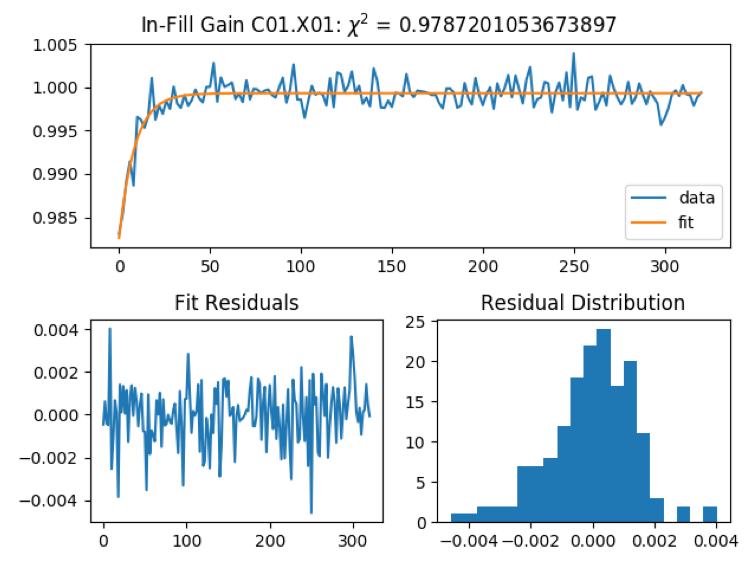
\includegraphics[width=.8\textwidth]{MatthiasInFill}
		    \caption[MatthiasInFill]{The top plot shows the in-fill gain sag function in orange from a fit to data in blue, for crystal 1 in calorimeter 1. The gain sag can be modeled effectively by a simple exponential function. By $\SI{30}{\mu s}$ the change in energy response is nearly only .1\%. The bottom two plots show the residuals of the fit. Plot made by Matthias Smith.}
		    \label{Fig:MatthiasInFill}
		\end{figure}

		For the error due to the amplitude, I applied multipliers on the amplitude of 0, 0.9, 0.95, 1, 1.05, 1.1, and 2. For the error due to the lifetime, I applied multipliers of 0.1, 0.9, 0.95, 1, 1.05, 1.1, and 2. The results of these scans are shown in Figure \ref{Fig:InFillGain}. I included the mulipliers of 0 (or 0.1) and 2 in order to calculate outer limits on the error. The multipliers of 2 resulted in a 7 ppb change on R due to the amplitude, and an 85 ppb change due to the lifetime. The change in R due to the multipliers of 0 or 0.1 were 6 ppb due to both the amplitude and lifetime. I calculate the systematic error on R as the quadrature sum of the separate pieces: 
		\begin{align}
			\delta R_{A} &= \delta\alpha_{A} \times \frac{dR}{d\alpha_{A}}, \\
			\delta R_{\tau} &= \delta\alpha_{\tau} \times \frac{dR}{d\alpha_{\tau}},
		\end{align}
		where $\delta\alpha_{A}$ and $\delta\alpha_{\tau}$ are the uncertainties on the gain sag amplitude and lifetime respectively. I assume that these errors are uncorrelated. I take the uncertainties on the amplitude and lifetime at 10\%. This leads to systematic errors on R of $0.1 \times \SI{57.9}{ppb} = \SI{5.8}{ppb}$ and $0.1 \times \SI{42.9}{ppb} = \SI{4.3}{ppb}$ respectively. In each of these cases, the uncertainty is the uncertainty on the applied parameters, and not the stability or precision of the energy response over the course of the fill. These added in quadrature results in a systematic error on R of 7.2 ppb.

		\begin{figure}[]
		\centering
		    \begin{subfigure}[t]{0.45\textwidth}
			    \centering
				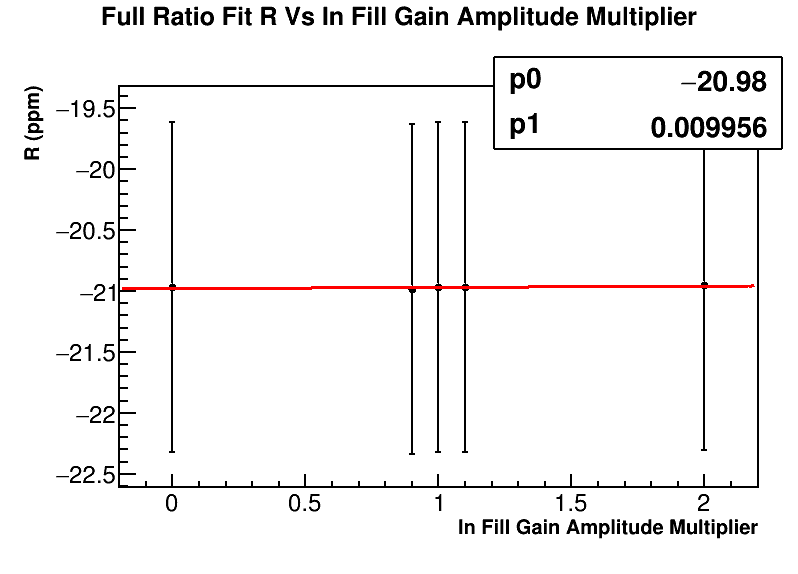
\includegraphics[width=\textwidth]{R_Vs_IFG_Amp_crystals}
			    \caption{Plotted is R vs the multiplier on the amplitude parameter in the gain sag function. A greater slope was observed when exluding the outer points, by over an order of magnitude. In order to be conservative I fit just the inner points. The slope is 57.9 ppb per unit amplitude.}
		    \end{subfigure}
		    \hspace{4mm}
		    \begin{subfigure}[t]{0.45\textwidth}
			    \centering
				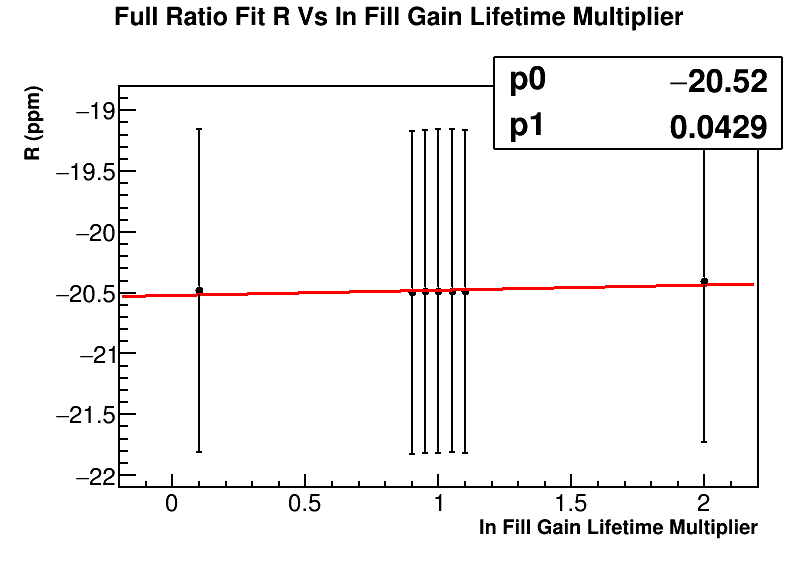
\includegraphics[width=\textwidth]{R_Vs_IFG_Tau_crystals}
			    \caption{Plotted is R vs the multiplier on the lifetime parameter in the gain sag function. The slope is 42.9 ppb per unit lifetime.}
		    \end{subfigure}% %you need this % here to add spacing between subfigures
		\caption[InFillGain]{Plotted are the fitted R values vs gain sag function parameter multipliers. In each case, these parameter multipliers were applied to each crystal individually, after undoing the gain sag correction done in the reconstruction. The fact that the outer points change the R value by so little indicates that the ratio fit is largely insensitive to the amplitude and lifetime of the gain function, as it is divided out.}
		\label{Fig:InFillGain}
		\end{figure}


	\subsection{Short Term Double Pulse (SDTP)}

		To determine the systematic effect from the SDTP correction, the path forward is to reconstruct the cluster with and without the correction and observe the change in R. I expect it to be small considering how small the in fill gain systematic error was.

	\subsection{Unseen/Unknown Gain Changes}

		More thought needs to be given on how any unseen gain changes might affect R.

\section{Sensitivity of \texorpdfstring{$\omega_{a}$}{} to pileup}
\label{Sec:SystematicPileup}

	The systematic error on R due to the pileup construction consists primarily of two parts, the error due to misconstruction of the amplitude and the phase of the pileup. I estimate the systematic error on R due to the pileup amplitude at 24.1 ppb, and to the pileup phase in pieces of 23.1 and 17.1 ppb. Adding these in quadrature results in a systematic error of 37.5 ppb.

	\subsection{Pileup Amplitude}

		The error due to the amplitude misconstruction was calculated by scanning over a pileup multiplier parameter, from 90\% of the calculated pileup amplitude to 110\%, as shown in Figure \ref{fig:PileupMultiplier}. The sensitivity of R to the amplitude was determined to be -553.4 ppb per unit amplitude. The uncertainty of the pileup amplitude construction was determined by fitting a parabola to the \chisq as a function of the pileup amplitude, and taking the width of that parabola as the uncertainty. This width is determined as the distance in X for the \chisq to rise by 1 from the minimum, also calculated as $\sqrt{2/(\chi^{2})''}$.

		\begin{figure}[h]
		\centering
		    \begin{subfigure}[t]{0.45\textwidth}
			    \centering
				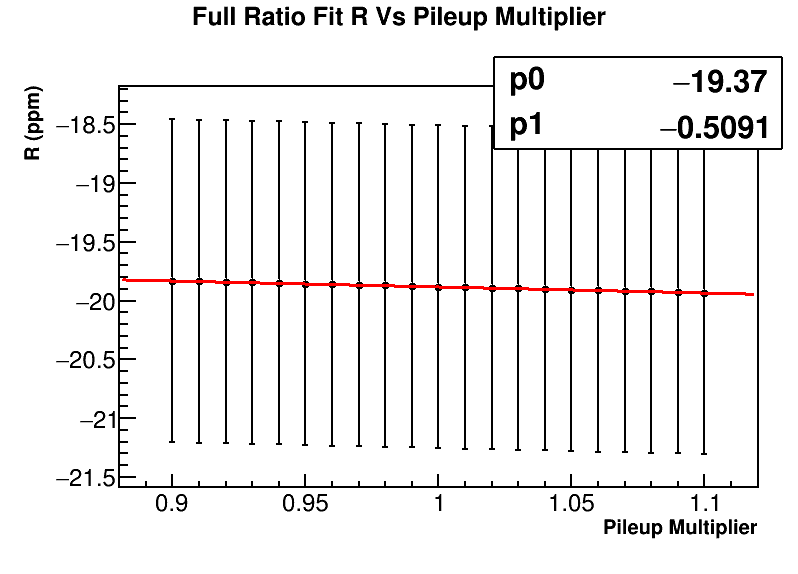
\includegraphics[width=\textwidth]{RatioCBO_R_Vs_PileupMultiplier_Canv}
			    \caption{Sensitivity of R vs the pileup amplitude. The slope is -553.4 ppb per unit amplitude.}
		    \end{subfigure}
		    \hspace{4mm}
		    \begin{subfigure}[t]{0.45\textwidth}
			    \centering
				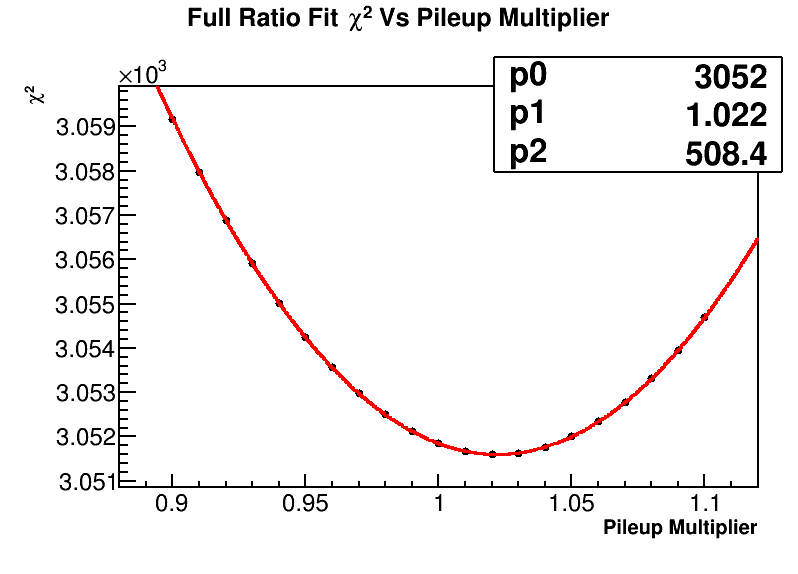
\includegraphics[width=\textwidth]{RatioCBO_Chi2_Vs_PileupMultiplier_Canv}
			    \caption{Plotted is the fitted \chisq vs the pileup amplitude. The fit equation used was $p2 \times (x - p1)^{2} + p0.$ The minimum lies at 0.9993.}
		    \end{subfigure}
		\caption[PileupMultiplier]{The significant plots to determine the pileup amplitude systematic error.}
		\label{fig:PileupMultiplier}
		\end{figure}

		This corresponds to an uncertainty of $\sqrt{1/526.5} = 0.0436$ or 4.36\%. The minimum of the \chisq plot is consistent with 1. (Note that this minimum flucuates with the random seed, and simply needs to be statistically consistent with 1). Then, calculating the systematic error on R due to the pileup amplitude construction as 
			\begin{align}
				\delta R_{pm} = \delta\alpha_{pm} \times \frac{dR}{d\alpha_{pm}}
			\end{align}
		where $\delta\alpha_{pm}$ is the uncertainty on the pileup amplitude, the systematic error on R is calculated as $0.0436 \times \SI{553.4}{ppb} = \SI{24.1}{ppb}$.

		Another technique to estimate the uncertainty of the pileup amplitude construction is to look at the offset of the high energy tail of the pileup subtracted energy spectrum from zero. Because however I've applied only the doublet correction, I know that the shape of the pileup spectrum is wrong by some amount, as evidenced in Figure \ref{fig:AddedEnergies}. While the pileup itself can multiplied by some scaling factor other than 1 in order to align the energy spectra slightly better, because the shape of the pileup correction is imperfect the offset calculation I believe is the wrong way to go about calculating this uncertainty in my case. The shape can be fixed by including the triplets and the doublet contamination in the shadow method, but that work is incomplete. Since the triplets are a 1\% effect relative to the doublets, and the contamination is of the same order, I believe the uncertainty of 4.36\% conservatively includes for this mismatch in shape and the omission of the triplets. Regardless, since the statistics of the 60H dataset is much larger than the order of the systematic effect for the pileup construction ($\mathcal{O}$(1 ppm) vs $\mathcal{O}$(10 ppb)), this is a fine assumption.

	\subsection{Pileup Phase}
	\label{SubSec:PileupPhase}

		The error on R due to the pileup phase construction was calculated by scanning over a pileup time shift parameter, where the pileup spectrum was shifted in time by some amount before subtraction. The sensitivity of R to this parameter is shown in Figure \ref{fig:PileupPhase}. It is unlikely that the entire pileup spectrum could be shifted by the offsets shown here, so this is a conservative estimate of the effect of the pileup phase on R. I then calculate the phase error as 
			\begin{align}
				\delta R_{pp} = \delta\alpha_{pp} \times \frac{dR}{d\alpha_{pp}}
			\end{align}
		where $\delta\alpha_{pp}$ is the uncertainty on the pileup phase. Conservatively estimating the uncertainty on the pileup phase as half the artificial deadtime at 3 ns, the systematic error on R is then calculated as $\SI{3}{ns} \times \SI{7.697}{ppb/ns} = \SI{23.1}{ppb}$. Figure \ref{fig:PileupTimeShiftFS} shows the change in R vs fit start times for pileup time shifted spectra vs the unshifted pileup time spectra. As shown the difference converges to zero as the level of pileup diminishes over the course of a fill.

		\begin{figure}[]
			\centering
			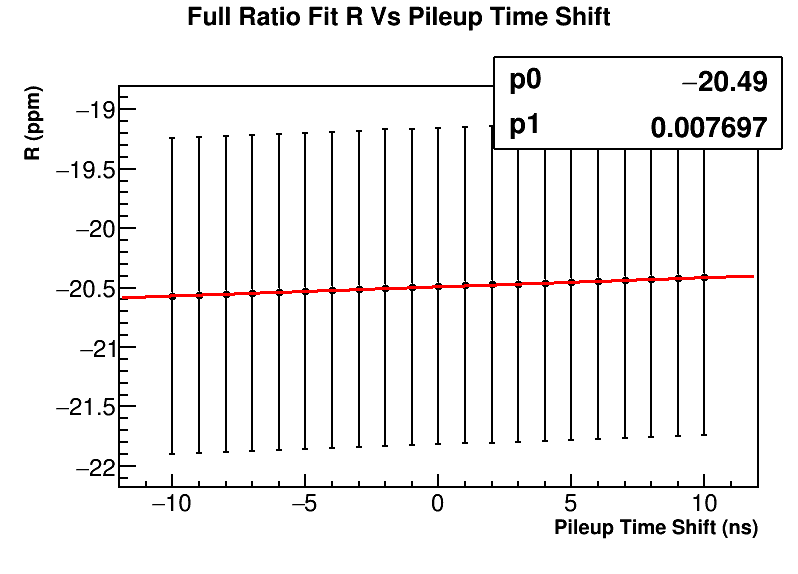
\includegraphics[width=.5\textwidth]{RatioCBO_R_Vs_PileupTimeShift_Canv}
		    \caption[PileupPhase]{Sensitivity of R vs the pileup phase. The slope is 7.697 ppb per ns.}
		    \label{fig:PileupPhase}
		\end{figure}

		\begin{figure}[]
			\centering
			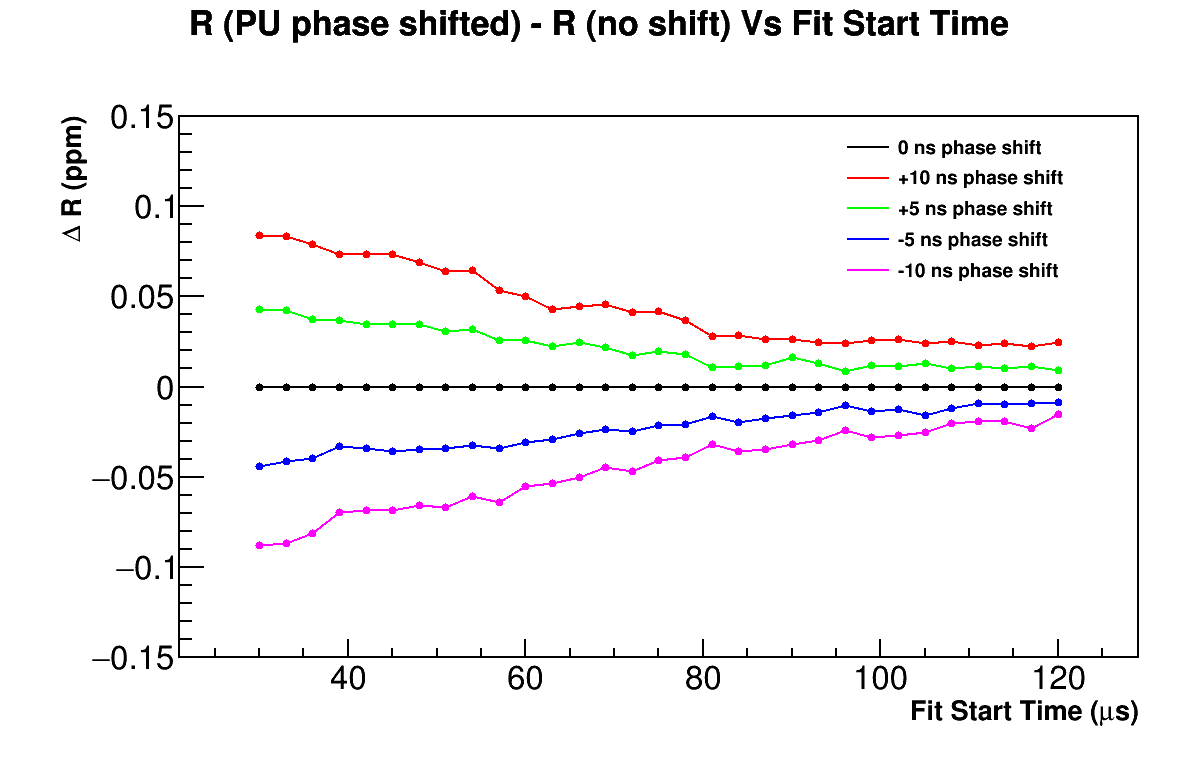
\includegraphics[width=.8\textwidth]{pileupTimeShiftComparison}
		    \caption[PileupTimeShiftFS]{Plotted is $\Delta R$ between pileup time shifted and unshifted results vs fit start time. The black line and points are by definition 0. As the fit start time increases and the pileup reduces, the $\Delta R$ points converge to zero as they should. Plot created on 5033A dataset.}
		    \label{fig:PileupTimeShiftFS}
		\end{figure}

		As mentioned in section Section \ref{Sec:PileupCorrection}, the energy of the pileup pulses may not actually be exactly equal to the sum of the pileup singlets. If the energy of the pileup pulses are systematically miscalculated, then doublets will be added or lost near the energy threshold applied when constructing the pileup spectrum. This leads to an additional error on the phase which needs to be included. With the energy of the pileup pulses calculated as
			\begin{align}
				E_{doublet} = C \cdot (E_{1} + E_{2}),
			\end{align}
		by scanning over the parameter C this error can be determined. The sensitivity of R to this pileup energy scaling parameter is shown in Figure \ref{fig:PileupEnergyScaling}, with a slope of -841.6 ppb per unit scaling parameter. The systematic error on R is calculated in the usual way,
			\begin{align}
				\delta R_{pe} = \delta\alpha_{pe} \times \frac{dR}{d\alpha_{pe}}
			\end{align}
		where $\delta\alpha_{pe}$ is the uncertainty on the pileup energy dependence. This uncertainty was calculated in the same manner as was done for the pileup amplitude, by fitting a parabola to the \chisq as a function of the energy scaling parameter, and it was determined to be 2.03\%. The systematic error on R is then calculated as $0.0203 \times \SI{841.6}{ppb} = \SI{17.1}{ppb}$.

		\begin{figure}[]
		\centering
		    \begin{subfigure}[t]{0.45\textwidth}
			    \centering
				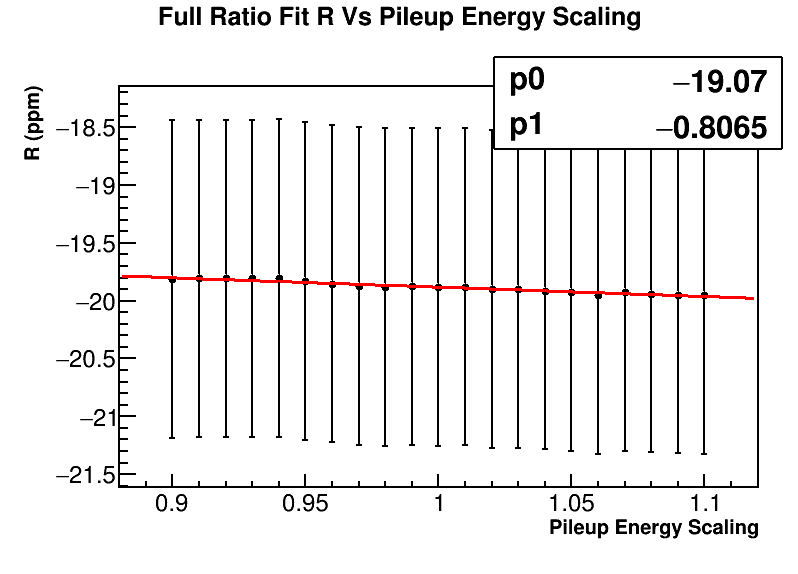
\includegraphics[width=\textwidth]{RatioCBO_R_Vs_PileupEnergyScaling_Canv}
			    \caption{Sensitivity of R vs the pileup energy scaling parameter. The slope is -841.6 ppb per unit energy scaling.}
		    \end{subfigure}
		    \hspace{4mm}
		    \begin{subfigure}[t]{0.45\textwidth}
			    \centering
				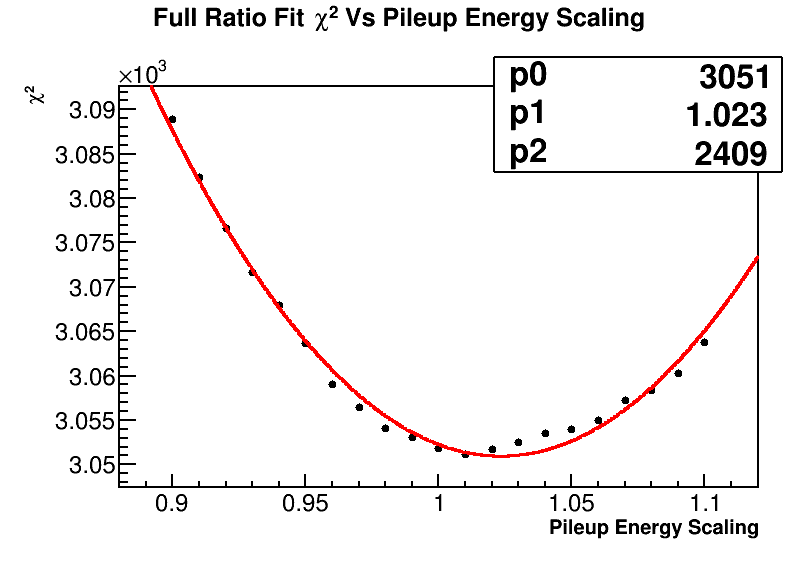
\includegraphics[width=\textwidth]{RatioCBO_Chi2_Vs_PileupEnergyScaling_Canv}
			    \caption{Plotted is the fitted \chisq vs the pileup energy scaling parameter. The fit equation used was $p2 \times (x - p1)^{2} + p0.$ The minimum lies at 1.013.}
		    \end{subfigure}
		\caption[PileupEnergyScaling]{The significant plots to determine a part of the pileup phase systematic error.}
		\label{fig:PileupEnergyScaling}
		\end{figure}


\section{Sensitivity of \texorpdfstring{$\omega_{a}$}{} to lost muons}
\label{Sec:SystematicLM}

	I estimate the systematic error on R due to the lost muon function at 29.9 ppb, and have yet to estimate the systemetic error due to the lost muon bias.

	\subsection{Lost muon function}
	\label{SubSec:LMFunc}

		As described in Section \ref{Sec:LM}, the lost muon function does not need to be included in the ratio fit. In order to calculate a systematic error from excluding the lost muon function, I added the function to the fit as described in that section. I fixed the value of the $\kappa_{loss}$ parameter to that determined from a T Method fit of the same data. The results can be seen in Figure \ref{fig:LMModuloPlot}. The final fitted R value differs from the non-LM fitted function by -29.9 ppb. Therefore I take the the systematic error from excluding the lost muon function as 29.9 ppb.

		\begin{figure}[]
			\centering
			\includegraphics[width=\textwidth]{ratioCBO_moduloPlot-lostmuonsfixed}
		    \caption[LMModuloPlot]{Fit results with the LM term included. The lost muon parameter has been fixed. The x axis is in units of $\mu$s modulo 100 $\mu$s, with successive portions of the data points and fit shifted downwards on the plot. The fit ranges from $\SI{30.2}{\mu s}$ to $\SI{650}{\mu s}$.}
		    \label{fig:LMModuloPlot}
		\end{figure}


	\subsection{Lost muon bias}

		If lost decay positrons (from lost muons) have different average \gmtwo phases than the measured decay positrons, there will be a changing \gmtwo phase over the course of a fill. This will produce a systematic effect on R, pulling its value. A study of this effect is beyond the scope of this report, and will be left out. However it should be noted that this error is likely sizeable, $\mathcal{O}(100)$ ppb or so.


\section{Sensitivity of \texorpdfstring{$\omega_{a}$}{} to CBO function}
\label{Sec:SystematicCBO}

	Results produced on the 5033A dataset. \\

	I estimate the systematic error on R due to the CBO frequency at 30 ppb, to the CBO envelope shape at 21.1 ppb, and to the fixed CBO lifetime at 12.1 ppb. Adding these in quadrature results in a systematic error of 38.6 ppb.

	\subsection{CBO Frequency}
	\label{Sec:CBOFreq}

	As described in Section \ref{Sec:CBO}, the CBO frequency as a function of time changes over the course of a fill. Shown in Figure \ref{fig:CBOFreqModel} is a comparison between the fitted CBO frequency parameter as a function of fit start time for a constant frequency vs a changing frequency. Without the changing frequency the fit behaves improperly. Because a specific model was chosen for the CBO frequency, there will be a systematic error on R that needs to be determined. James Mott examined the frequency function he derived from the data in greater detail in \DB{15376}, where he considered parameter correlations in Equation \ref{Eqn:CBOFreq} and subsequent effects on the overall function. He found that errors were small, parameters were highly correlated, and that the CBO frequency function was very well constrained, as well as comparable between stations 12 and 18, and the 60H and 9d datasets. 

	In order to determine the systematic error on R, I simply varied the individual fixed parameters in the CBO frequency function $\{\Delta\omega, A, \tau_{A}, B, \tau_{B}\}$, by $\pm 2 \sigma$, where the errors on the parameters were taken from \DB{15376}. I also fit the data with the station 18 parameters. Even though the frequency parameters are highly correlated, varying them individually should be a conservative method for determining the overall systematic error on R. I found a 25 ppb difference in the fitted R value for the station 18 parameters, as compared to the station 12 parameters, primarily due to the different ``A'' value, and differences of order 5 ppb or less for the rest of the parameters. Adding them in quadrature resulted in an error of approximately 27.3 ppb. In order to be slightly more conservative, I estimate the systematic error on R due to the frequency at 30 ppb.

		\begin{figure}[]
		\centering
		    \begin{subfigure}[t]{0.45\textwidth}
			    \centering
				\includegraphics[width=\textwidth]{fixed-wcbo-vs-fs}
			    \caption{Fixed CBO frequency.}
		    \end{subfigure}
		    \hspace{4mm}
		    \begin{subfigure}[t]{0.45\textwidth}
			    \centering
				\includegraphics[width=\textwidth]{RatioCBO_omega_cbo_FS_Canv}
			    \caption{Changing CBO frequency.}
		    \end{subfigure}
		\caption[CBOFreqModel]{Fit start time scans for the CBO frequency parameter with a fixed frequency (left) and for the tracker model frequency (right). With the inclusion of the changing frequency over time, the fit parameter becomes stable as a function of fit start time. (Note that the plot on the left was produced with the 5033A dataset, and the fitted parameter was in different units at the time of creation.)}
		\label{fig:CBOFreqModel}
		\end{figure}


	\subsection{CBO Shape}
	\label{SubSec:CBOShape}

		If the shape of the CBO in the fit function is wrong, then there will be a systematic error on R. Because I get good fits and the CBO parameters are stable vs fit start time, the possbile changes to the envelope are limited, compared to the envelope used as shown in Equation \ref{eqn:CBO}. Possible changes to the envelope include those functions as shown in Figure \ref{fig:CBOShapeAmplitude}, an exponential plus a constant and then an exponential times another oscillatory term. Both new envelopes were determined from tracker analysis fits to the CBO amplitude. Both changes to the envelope amplitude were tried in the fitting function, with changes in R of $\SI{-21.1}{ppb}$ and $\SI{-9.6}{ppb}$ respectively, though neither showed any improvement in the fit. (In the latter the period of the oscillatory term was fixed and the other parameters were allowed to float.) I take the latter value of $\SI{21.1}{ppb}$ as the systematic error on R due to the shape.

		\begin{figure}[]
			\centering
			\includegraphics[width=.7\textwidth]{AmplFitOptions}
		    \caption[CBOShapeAmplitude]{Plotted is the CBO amplitude as a function of time from the tracker analysis. Three separate fit functions were used with varying degrees of success to characterize the envelope shape of the CBO (excepting the cosine modulation part). A Gaussian fit was tried with no success. The amplitude isn't fully understood at early times. The period T/$2\pi$ has a value of $\SI{114.5}{\mu s}$. Plot producd by James Mott.}
		    \label{fig:CBOShapeAmplitude}
		\end{figure}

	\subsection{CBO Lifetime}

		I plan on removing this systematic when refitting new dataset, with the cbo lifetime floating. \\

		Because the CBO lifetime has been fixed in the fit, there is a systematic error on R. Scanning over various values of the fixed CBO lifetime allows this error to be calculated. The resulting curve of R vs the CBO lifetime turns out not to be linear, as shown in Figure \ref{fig:CBOLifetime}. Taking the uncertainty on the CBO lifetime as the error produced by the T Method fit, approximately $\SI{16}{\mu s}$, and looking at the change in R for CBO lifetime values of $180 \pm \SI{16}{\mu s}$, the systematic error on R is taken as the larger of the two at 12.1 ppb.

		\begin{figure}[]
			\centering
			\includegraphics[width=.6\textwidth]{RatioCBO_R_Vs_tau_cbo_Canv}
		    \caption[CBOLifetime]{Plotted is the fitted R value as a function of the CBO lifetime, which has been fixed in the full ratio fit. The error bars have been removed from the plot in order to show the shape of the curve better. The points have been fitted to an exponential function which lines up nicely, $p_{0} e^{-t/p_{1}} + p_{2}$.}
		    \label{fig:CBOLifetime}
		\end{figure}

	\subsection{CBO Fit Terms}
	\label{SubSec:CBOFitTerms}

		I plan on estimating a systematic error due to excluded CBO terms (like the CBO phase term) with the new dataset.



\section{Sensitivity of \texorpdfstring{$\omega_{a}$}{} to VW function}
\label{Sec:SystematicVW}

	As described in Section \ref{Sec:VW}, the vertical waist does not need to be included in the ratio fit. In order to calculate a systematic error from excluding the VW, I added the VW to the fit as described in that section, with an exponentially decaying cosine term. Since the fit is unstable in regards to the amplitude and lifetime parameters, I fixed them to values determined from a T Method fit of the same data. The results can be seen in Figure \ref{fig:VWModuloPlot}. The final fitted R value differs from the non-VW fitted function by less than 1 ppb. This is unsurprising since I'm trying to fit an effect which does not exist in the ratio.

	\begin{figure}[]
		\centering
		\includegraphics[width=\textwidth]{ratioCBO_moduloPlot-VW}
	    \caption[VWModuloPlot]{Fit results with the VW term included. The VW parameters have been fixed to values determined from a T Method fit to the data. The x axis is in units of $\mu$s modulo 100 $\mu$s, with successive portions of the data points and fit shifted downwards on the plot. The fit ranges from $\SI{30.2}{\mu s}$ to $\SI{650}{\mu s}$.}
	    \label{fig:VWModuloPlot}
	\end{figure}



\section{Sensitivity of \texorpdfstring{$\omega_{a}$}{} to various effects}

	\subsection{\gmtwo Period Guess}
	\label{SubSec:gm2Guess}

		To perform the ratio method, the \gmtwo period needs to be known a priori to high precision. This is because this value is used when time shifting the individual counts before filling the ratio histograms. By scanning over various \gmtwo period guesses the dependence of R on $T_{a}$ can be determined, as shown in Figure \ref{fig:gm2PeriodGuess}. The systematic error can then be calculated as 
			\begin{align}
				\delta R_{period} = \delta\alpha_{period} \times \frac{dR}{d\alpha_{period}}
			\end{align}
		where $\delta\alpha_{period}$ is the uncertainty on $T_{a}$. 

		Since the period that the counts need to be shifted by is already modified by the hardware blinding, it is technically the hardware shifted \gmtwo period that we want to use. As described in \cite{ClockManual}, the calorimeter digitizers use a ``40'' MHz clock which has been blinded to a value in the range of 39.997 to 39.999 MHz. This corresponds to a 75 ppm range in the frequency we're after, in a uniform distribution. Calculating the uncertainty from said uniform distribution and adding it in quadrature with a conservative 10 ppm uncertainty in the guess on the true \gmtwo period: 
			\begin{align}
				\delta\alpha_{period} = \sqrt{(75)^{2}/12 + 10^{2}} = \SI{23.8}{ppm}
			\end{align}
		This results in a systematic error of $\SI{23.8}{ppm} \times \SI{1.16e-4}{ppm/ppm} = \SI{2.8}{ppb}$.

		\begin{figure}[]
			\centering
			\includegraphics[width=.6\textwidth]{RatioCBO_R_Vs_gm2PeriodGuess_Canv}
		    \caption[gm2PeriodGuess]{Fitted R value as a function of the ppm level offset from the default guess used for the \gmtwo period, \ref{eq:Ta}. Error bars have been removed from this plot, otherwise it appears as a flat line. There appears to be a noticeable oscillation in the points at \gmtwo period guesses beyond the range of -25 ppm - +25 ppm, therefore the fit has been restricted to that range. The slope is .116 ppb per ppm offset in $T_{a}$.}
		    \label{fig:gm2PeriodGuess}
		\end{figure}

	\subsection{Lifetime used in weighting}
	\label{SubSec:LifetimeWeighting}

		Similarly to the \gmtwo period guesses used when constructing the time spectra for the ratio method, the lifetime of the muon is used when splitting the counts into the various histograms with different weights, as seen in Equation \ref{Eqn:Weighting}. To check for a systematic effect on R from getting this lifetime wrong, I scanned over a range of such lifetimes around the default value used, $\SI{64.4}{\mu s}$. As shown in Figure \ref{fig:weightingLifetime}, the slope is 4.015 ppb per $\mu$s. Since the uncertainty on the lifetime is much less than a microsecond, this systematic error is neglible.

		\begin{figure}[]
			\centering
			\includegraphics[width=.6\textwidth]{RatioCBO_R_Vs_weightingLifetime_Canv}
		    \caption[weightingLifetime]{Fitted R value as a function of the lifetime used in the weighting of counts into histograms. Error bars have been removed from this plot, otherwise it appears as a flat line. The slope is 4.015 ppb per $\mu$s.}
		    \label{fig:weightingLifetime}
		\end{figure}


\clearpage

	\subsection{Bin Width}

		The bin width of the histograms is chosen to eliminate the fast rotation signal. The spread in bin widths corresponding to the range of cyclotron frequencies in the data is from about 148.9 ns to about 149.6 ns, with 149.2 ns being the peak of the distribution. R as a function of bin width is shown in Figure \ref{fig:BinWidth}. As shown there doesn't appear to be any significant trend for R with respect to the bin width. The randomization of counts also ties in with the bin width, as counts will be shifted from one bin to another based on where the bin edges fall. For these reasons I forgo any systematic error calculation due to the choice of bin width itself. See the following section on the randomization and the systematic error relating to it.

		\begin{figure}[]
		    \begin{subfigure}[t]{0.45\textwidth}
			    \centering
				\includegraphics[width=\textwidth]{BinWidthComparison_R}
			    \caption{In graph format. As can be seen there is no clear trend for R with respect to the bin width.}
		    \end{subfigure}
		    \hspace{4mm}
		    \begin{subfigure}[t]{0.45\textwidth}
			    \centering
				\includegraphics[width=\textwidth]{BinWidthComparison_R_hist}
			    \caption{In histogram format. The RMS spread is 99.9 ppb.}
		    \end{subfigure}% %you need this % here to add spacing between subfigures
		\caption[BinWidth]{Plotted are fitted R values for varying bin widths ranging from 148.9 ns to 149.6 ns in steps of .1 ns.}
		\label{fig:BinWidth}
		\end{figure}

	\subsection{Randomization}
	\label{Sec:Randomization}

		In the histogramming phase of my analysis, random seeds are used in two places. One for the randomization of counts into the 4 separate datasets that go into the ratio, and one for the time randomization to reduce the fast rotation. It's necessary to make sure that results are consistent among random seeds, and that the final answer wasn't a particularly fortuitous or disastrous choice. In order to test this I performed fits with 50 different random seeds, the $\chi^{2}/NDF$ and fitted R values of which are plotted in Figure \ref{fig:RandomSeeds}. Results are consistent and very much within error of each other. I also performed fit start scans for a couple of the random seeds as an extra check to make sure the fitting was behaving consistently as shown in Figures \ref{fig:RandomSeedFitStartScansChi2} and \ref{fig:RandomSeedFitStartScansR}. I've included plots of the other fit parameters as a function of random seed in Figures \ref{fig:RandomSeedsPars1} - \ref{fig:RandomSeedsPars3}.

		\begin{figure}[]
		\centering
		    \begin{subfigure}[t]{0.45\textwidth}
			    \centering
				\includegraphics[width=\textwidth]{RatioCBO_Chi2NDF_Vs_Iter_Canv_hist}
			    \caption{$\chi^{2}$/NDF values for 50 random seeds. The mean is near 1.}
		    \end{subfigure}
		    \hspace{4mm}
		    \begin{subfigure}[t]{0.45\textwidth}
			    \centering
				\includegraphics[width=\textwidth]{RatioCBO_R_Vs_Iter_Canv_hist}
			    \caption{R values for 50 random seeds. The mean is -20.38 ppm and the RMS is 170.5 ppb.}
			\label{Subfig:RVsRandomSeed}
		    \end{subfigure}% %you need this % here to add spacing between subfigures
		\caption[RandomSeeds]{Plotted are the $\chi^{2}$/NDF and fitted R values for 50 random seeds.}
		\label{fig:RandomSeeds}
		\end{figure}

		\begin{figure}[]
		\centering
		    \begin{subfigure}[t]{0.45\textwidth}
			    \centering
				\includegraphics[width=\textwidth]{RatioCBO_Chi2NDF_Vs_FS_canv-Seed0}
			    \caption{Seed 1}
		    \end{subfigure}
		    \begin{subfigure}[t]{0.45\textwidth}
			    \centering
				\includegraphics[width=\textwidth]{RatioCBO_Chi2NDF_Vs_FS_canv-Seed1}
			    \caption{Seed 2}
		    \end{subfigure}% %you need this % here to add spacing between subfigures
		    \vspace{4mm}
		    \begin{subfigure}[t]{0.45\textwidth}
			    \centering
				\includegraphics[width=\textwidth]{RatioCBO_Chi2NDF_Vs_FS_canv-Seed2}
			    \caption{Seed 3}
		    \end{subfigure}
		    \begin{subfigure}[t]{0.45\textwidth}
			    \centering
				\includegraphics[width=\textwidth]{RatioCBO_Chi2NDF_Vs_FS_canv-Seed3}
			    \caption{Seed 4}
		    \end{subfigure}% %you need this % here to add spacing between subfigures
		\caption[RandomSeedFitStartScansChi2]{Fit start time scans for the \chisq for four random seeds of the randomization of the same dataset. Compare to Figure \ref{fig:Chi2FSScan}. The general behaviour of the fits vs fit start time is consistent and relatively the same, but as is seen the scans can rise and fall at different points due to the choice of randomization.}
		\label{fig:RandomSeedFitStartScansChi2}
		\end{figure}

		\begin{figure}[]
		\centering
		    \begin{subfigure}[t]{0.45\textwidth}
			    \centering
				\includegraphics[width=\textwidth]{RatioCBO_R_FS_canv-Seed0}
			    \caption{Seed 1}
		    \end{subfigure}
		    \begin{subfigure}[t]{0.45\textwidth}
			    \centering
				\includegraphics[width=\textwidth]{RatioCBO_R_FS_canv-Seed1}
			    \caption{Seed 2}
		    \end{subfigure}% %you need this % here to add spacing between subfigures
		    \vspace{4mm}
		    \begin{subfigure}[t]{0.45\textwidth}
			    \centering
				\includegraphics[width=\textwidth]{RatioCBO_R_FS_canv-Seed2}
			    \caption{Seed 3}
		    \end{subfigure}
		    \begin{subfigure}[t]{0.45\textwidth}
			    \centering
				\includegraphics[width=\textwidth]{RatioCBO_R_FS_canv-Seed3}
			    \caption{Seed 4}
		    \end{subfigure}% %you need this % here to add spacing between subfigures
		\caption[RandomSeedFitStartScansR]{Fit start time scans for the fitted R parameter for four random seeds of the randomization of the same dataset. The general behaviour of the R value vs fit start time is very consistent between seeds.}
		\label{fig:RandomSeedFitStartScansR}
		\end{figure}

		If the reported final answer on R is that of a single fit, then I believe there should be no systematic error on R due to the randomization. Such an error should be contained within the statistical error of the fitted parameter. If however the reported final answer is the average R value from many random seeds, then I can see why one might want to add in such a systematic error. For the latter case I calculate the systematic error on R as:
			\begin{align}
				\delta R_{rand} = \sigma(R)/\sqrt{N-1},
			\label{Eqn:Rand}
			\end{align}
		where $\sigma(R)$ is the RMS spread in R and N is the number of random seeds fitted, in this case 50. Therefore with an RMS on R of 170.5 ppb, the systematic error on the average R due to the randomization is 24.4 ppb. Perhaps the best thing to do is to report the fitted R value from a single fit that is closest to the mean, to avoid this error entirely while remaining closest to the average value.

		\begin{figure}[]
		\centering
		    \begin{subfigure}[t]{0.45\textwidth}
			    \centering
				\includegraphics[width=\textwidth]{RatioCBO_Chi2NDF_Vs_Iter_Canv_hist}
			    \caption{$\chi^{2}$/NDF}
		    \end{subfigure}
		    \hspace{4mm}
		    \begin{subfigure}[t]{0.45\textwidth}
			    \centering
				\includegraphics[width=\textwidth]{RatioCBO_PVal_Vs_Iter_Canv}
			    \caption{P value}
		    \end{subfigure}% %you need this % here to add spacing between subfigures
		   	\vspace{4mm}
		    \begin{subfigure}[t]{0.45\textwidth}
			    \centering
				\includegraphics[width=\textwidth]{RatioCBO_R_Vs_Iter_Canv}
			    \caption{R in graph format.}
		    \end{subfigure}
		    \hspace{4mm}
		    \begin{subfigure}[t]{0.45\textwidth}
			    \centering
				\includegraphics[width=\textwidth]{RatioCBO_R_Vs_Iter_Canv_hist}
			    \caption{R in histogram format.}
		    \end{subfigure}% %you need this % here to add spacing between subfigures
		\caption[RandomSeedsPars1]{Plotted are various fitted parameters for 50 different random seeds in graph and histogram format.}
		\label{fig:RandomSeedsPars1}
		\end{figure}

		\begin{figure}[]
		\centering
		    \begin{subfigure}[t]{0.45\textwidth}
			    \centering
				\includegraphics[width=\textwidth]{RatioCBO_A_Vs_Iter_Canv}
			    \caption{A in graph format.}
		    \end{subfigure}
		    \hspace{4mm}
		    \begin{subfigure}[t]{0.45\textwidth}
			    \centering
				\includegraphics[width=\textwidth]{RatioCBO_A_Vs_Iter_Canv_hist}
			    \caption{A in histogram format.}
		    \end{subfigure}% %you need this % here to add spacing between subfigures
		   	\vspace{4mm}
		    \begin{subfigure}[t]{0.45\textwidth}
			    \centering
				\includegraphics[width=\textwidth]{RatioCBO_phi_Vs_Iter_Canv}
			    \caption{\gmtwo phase in graph format.}
		    \end{subfigure}
		    \hspace{4mm}
		    \begin{subfigure}[t]{0.45\textwidth}
			    \centering
				\includegraphics[width=\textwidth]{RatioCBO_phi_Vs_Iter_Canv_hist}
			    \caption{\gmtwo phase in histogram format.}
		    \end{subfigure}% %you need this % here to add spacing between subfigures
		   	\vspace{4mm}
		   	\begin{subfigure}[t]{0.45\textwidth}
			    \centering
				\includegraphics[width=\textwidth]{RatioCBO_omega_cbo_Vs_Iter_Canv}
			    \caption{CBO frequency in graph format.}
		    \end{subfigure}
		    \hspace{4mm}
		    \begin{subfigure}[t]{0.45\textwidth}
			    \centering
				\includegraphics[width=\textwidth]{RatioCBO_omega_cbo_Vs_Iter_Canv_hist}
			    \caption{CBO frequency in histogram format.}
		    \end{subfigure}% %you need this % here to add spacing between subfigures
		\caption[RandomSeedsPars2]{Plotted are various fitted parameters for 50 different random seeds in graph and histogram format.}
		\label{fig:RandomSeedsPars2}
		\end{figure}

		\begin{figure}[]
		\centering
		    \begin{subfigure}[t]{0.45\textwidth}
			    \centering
				\includegraphics[width=\textwidth]{RatioCBO_tau_cbo_Vs_Iter_Canv}
			    \caption{CBO lifetime in graph format.}
		    \end{subfigure}
		    \hspace{4mm}
		    \begin{subfigure}[t]{0.45\textwidth}
			    \centering
				\includegraphics[width=\textwidth]{RatioCBO_tau_cbo_Vs_Iter_Canv_hist}
			    \caption{CBO lifetime in histogram format.}
		    \end{subfigure}% %you need this % here to add spacing between subfigures
		   	\vspace{4mm}
		    \begin{subfigure}[t]{0.45\textwidth}
			    \centering
				\includegraphics[width=\textwidth]{RatioCBO_A_cbo-N_Vs_Iter_Canv}
			    \caption{CBO N amplitude in graph format.}
		    \end{subfigure}
		    \hspace{4mm}
		    \begin{subfigure}[t]{0.45\textwidth}
			    \centering
				\includegraphics[width=\textwidth]{RatioCBO_A_cbo-N_Vs_Iter_Canv_hist}
			    \caption{CBO N amplitude in histogram format.}
		    \end{subfigure}% %you need this % here to add spacing between subfigures
		   	\vspace{4mm}
		   	\begin{subfigure}[t]{0.45\textwidth}
			    \centering
				\includegraphics[width=\textwidth]{RatioCBO_phi_cbo-N_Vs_Iter_Canv}
			    \caption{CBO N phase in graph format.}
		    \end{subfigure}
		    \hspace{4mm}
		    \begin{subfigure}[t]{0.45\textwidth}
			    \centering
				\includegraphics[width=\textwidth]{RatioCBO_phi_cbo-N_Vs_Iter_Canv_hist}
			    \caption{CBO N phase in histogram format.}
		    \end{subfigure}% %you need this % here to add spacing between subfigures
		\caption[RandomSeedsPars3]{Plotted are various fitted parameters for 50 different random seeds in graph and histogram format.}
		\label{fig:RandomSeedsPars3}
		\end{figure}


	\subsection{Bunch Number}

		Each fill during normal data taking comes from one of eight separate muon bunches. Each individual bunch, due to the nature of the particle production and upstream beamline effects, likely has separate properties. In order to explore this the fit results can be examined as a function of bunch number. The fit results are shown in Figures \ref{fig:BunchNumChi2}, \ref{fig:BunchNumPars}, and \ref{fig:BunchNumParsCBO}. As can be seen in the first figure, it appears that the goodness-of-fit as a function of bunch number is not quite adequate, with most points being above 1. The fitted parameter values for the different bunches shown in the latter figures appear for the most part consistent, with some clear differences between the different bunches. This is especially evident in Figure \ref{SubFig:gm2PhaseBunch}, where the \gmtwo phase is clearly different between bunches. This could potentially lead to a systematic error on R, for example due to different lost muon characteristics per bunch and thus a changing average \gmtwo phase over the course of a fill. It is nice to see however that the average R value and \gmtwo phases between the different bunches are very consistent with the results from the bunch sum fit. The other parameters are all consistent as well to different degrees. This is only a cursory look at the analysis results on a per bunch basis, and the systematic effects on R (if indeed there are any) have yet to be explored in any great detail.

		\begin{figure}[]
			\centering
			\includegraphics[width=.6\textwidth]{RatioCBO_Chi2NDF_Vs_BunchNum_Canv}
		    \caption[BunchNumChi2]{Plotted are \chisq per degree of freedom values for the different bunch numbers. The point at bunch number 8 is the fit result from all bunches added together. The blue dashed line is set at the added bunch number result.}
		    \label{fig:BunchNumChi2}
		\end{figure}

		\begin{figure}[]
		\centering
		    \begin{subfigure}[t]{0.4\textwidth}
			    \centering
				\includegraphics[width=\textwidth]{RatioCBO_R_Vs_BunchNum_Canv}
			    \caption{Fitted R values as a function of bunch number.}
		    \end{subfigure}
		    \hspace{4mm}
		    \begin{subfigure}[t]{0.4\textwidth}
			    \centering
				\includegraphics[width=\textwidth]{RatioCBO_phi_Vs_BunchNum_Canv}
			    \caption{Fitted \gmtwo phase values as a function of bunch number.}
			    \label{SubFig:gm2PhaseBunch}
		    \end{subfigure}% %you need this % here to add spacing between subfigures
			\vspace{4mm}
		    \begin{subfigure}[t]{0.4\textwidth}
			    \centering
				\includegraphics[width=\textwidth]{RatioCBO_A_Vs_BunchNum_Canv}
			    \caption{Fitted A values as a function of bunch number.}
		    \end{subfigure}
		\caption[BunchNumPars]{Plotted are the main fitted parameter values for the different bunch numbers. The point at bunch number 8 is the fit result from all bunches added together. The blue dashed line is set at the added bunch number result, and the red line is the fit to the individual bunches excluding the final point.}
		\label{fig:BunchNumPars}
		\end{figure}

		\begin{figure}[]
		\centering
		    \begin{subfigure}[t]{0.4\textwidth}
			    \centering
				\includegraphics[width=\textwidth]{RatioCBO_omega_cbo_Vs_BunchNum_Canv}
			    \caption{Fitted CBO frequency values as a function of bunch number.}
		    \end{subfigure}
		    \hspace{4mm}
		    \begin{subfigure}[t]{0.4\textwidth}
			    \centering
				\includegraphics[width=\textwidth]{RatioCBO_tau_cbo_Vs_BunchNum_Canv}
			    \caption{Fitted CBO lifetime values as a function of bunch number. Bunches 6 and 7 hit the upper fit limit of $\SI{500}{\mu s}$.}
		    \end{subfigure}% %you need this % here to add spacing between subfigures
			\vspace{4mm}
		    \begin{subfigure}[t]{0.4\textwidth}
			    \centering
				\includegraphics[width=\textwidth]{RatioCBO_phi_cbo-N_Vs_BunchNum_Canv}
			    \caption{Fitted CBO phase values as a function of bunch number.}
		    \end{subfigure}
		    \hspace{4mm}
		    \begin{subfigure}[t]{0.4\textwidth}
			    \centering
				\includegraphics[width=\textwidth]{RatioCBO_A_cbo-N_Vs_BunchNum_Canv}
			    \caption{Fitted CBO N amplitude values as a function of bunch number.}
		    \end{subfigure}% %you need this % here to add spacing between subfigures
			\vspace{4mm}
		\caption[BunchNumParsCBO]{Plotted are the fitted CBO parameter values for the different bunch numbers. Some of the fitted parameters have large error bars, indicating that the fit had trouble fitting the CBO parameters. The point at bunch number 8 is the fit result from all bunches added together. The blue dashed line is set at the added bunch number result, and the red line is the fit to the individual bunches excluding the final point.}
		\label{fig:BunchNumParsCBO}
		\end{figure}


\clearpage

\section{Final Systematic Uncertainty Table}

The calculated systematic errors for the 60H dataset are shown in Table \ref{Tab:Systematics}. As a reminder, not all systematic uncertainty evaluations are fully completed. Here we see that...


\begin{table}[H]
\centering
\setlength\tabcolsep{10pt}
\renewcommand{\arraystretch}{1.2}
\begin{tabular*}{.5\linewidth}{@{\extracolsep{\fill}}|lG|}
  \hline
  	\multicolumn{2}{|c|}{\textbf{Summary of Systematic Errors}} \\
  \hline\hline
    Systematic Error 		& \multicolumn{1}{c|}{\SI{60}{H}} \\
  \hline
	Gain 			 		&  7.2   \\
	Pileup     	     		&  37.5  \\
	Lost Muons*             &  29.9  \\
	CBO      		 		&    \\
	VW 			     		&  \multicolumn{1}{c|}{$<1$} \\
	% Bin Width        		&    \\
	Randomization    		&  24.4  \\
	% Bunch Number     		&        \\
	Other* 				  	&  2.8   \\
  \hline\hline		
  	Total   	     		&    \\
  \hline
\end{tabular*}
\caption{Systematic error table for the 60H dataset. All units are in ppb. The `*'s indicate that significant work still needs to be done in the error estimation. The lack of a `*' does not preclude future work on the rest of the systematic errors. }
\label{Tab:Systematics}
\end{table}







%!TEX root = ../BU_60H_Unblinding_Report.tex

\graphicspath{ {Figures/TMethod/Main/} {Figures/TMethod/ResidualsFFT/} {Figures/TMethod/Comparison/} {Figures/TMethod/RandomSeeds/} }

\chapter{T Method Fit}
\label{Ch:TMethod}

While not the main focus of my analysis, I also perform a T method fit to the data along with the ratio fit. This is useful as a comparison to the ratio method results, and can also provide useful parameter information that the ratio method has trouble getting at. I do not perform systematic studies, and only perform analysis checks like fit start time scans to verify that the T method fit is working correctly. In my T method fit, I include all CBO terms except the $N_{2cbo}$ term, the vertical waist, and lost muons, as described in Chapter \ref{Ch:Procedures}, for a total of 18 fit parameters. The same fit start and end times as used in the ratio fit of $\SI{30.2}{\mu s} - \SI{650}{\mu s}$ are used here as well.

The results for a T-Method fit are shown in Figure \ref{fig:TMethod_moduloPlot}, with a table of the results with parameter information shown in Table \ref{Tab:FitParamsTMethod}. The correlation matrix for the T-Method fit is shown in Table \ref{Tab:CorrMatTMethod} and plotted in Figure \ref{fig:CorrelationMatrixTMethod}. Residuals and FFTs of the T method fit results are included for posterity in Figures \ref{fig:fitResidual_TMethod} - \ref{fig:FFTComparison_TMethod}. Note that the errors on the VW amplitude and phase are large, seemingly indicating that the VW does not need to be included in the fit. If it is excluded however, then the VW peak in the FFT of the residuals reappears, therefore it is left in the fit. Preliiminary tests with different random seeds indicate that there is a large effect on the degree of cancellation of the fast rotation and the subsequent values of the fitted VW parameters.

A comparison between the ratio and T-Method results are shown in Table \ref{Tab:FitComparison}. There is a slight difference in data that is fitted between the T method and the ratio method. Because of the time shifting that is done in the ratio method, there is a quarter \gmtwo periods worth of data starting at $\SI{30.2}{\mu s}$ that is replaced by data before $\SI{30.2}{\mu s}$. This shouldn't change much but should be kept in mind when comparing the results.

	\begin{figure}[]
		\centering
		\includegraphics[width=\textwidth]{Figures/TMethod/Main/TMethod_moduloPlot}
		\includegraphics[width=\textwidth]{TMethod_moduloPlot.png}
	    \caption[TMethod_moduloPlot]{Final fit result for the 60 hour dataset for a T method fit. The x axis is in units of $\mu$s modulo 100 $\mu$s, with successive portions of the data points and fit shifted downwards on the plot. R is blinded locally. The fit ranges from $\SI{30.2}{\mu s}$ to $\SI{650}{\mu s}$.}
	    \label{fig:TMethod_moduloPlot}
	\end{figure}

	\begin{table}[]
	\centering
	\setlength\tabcolsep{10pt}
	\renewcommand{\arraystretch}{1.2}
	\begin{tabular*}{.85\linewidth}{@{\extracolsep{\fill}}|l|l|c|c|}
	  \hline
	  	\multicolumn{4}{|c|}{\textbf{T-Method Fit Results}} \\
	  \hline\hline
	  	\multicolumn{2}{|c}{$\chi^{2}$/NDF}       				&  \multicolumn{2}{c|}{$4083/4137$}  \\
	  	\multicolumn{2}{|c}{P value}         	 				&  \multicolumn{2}{c|}{$0.7211$}  \\
	  \hline\hline
	  	Parameter & Descriptor & Value & Error \\
	  \hline
		$N_{0}$    			  & Number  	    			&  $\SI{3.452e+06}{}$ & $\SI{271.5}{}$ \\
		$\tau$    			  & Muon Lifetime $(\mu s)$ 	&  $\SI{64.44}{}$ & $\SI{0.0038}{}$ \\
		$A$    			 	  & Asymmetry  	    			&  $\SI{0.3704}{}$ & $\SI{4.396e-05}{}$ \\
		$R$     			  & R (ppm, blinded)   	 		&  $\SI{-20.450}{}$ & $\SI{1.311}{}$ \\
		$\phi$   			  & \gmtwo Phase         		&  $\SI{2.091}{}$ & $\SI{2.161e-4}{}$ \\
		$\omega_{cbo}$   	  & CBO Frequency $(MHz)$       &  $\SI{0.367}{}$ & $\SI{6.936e-05}{}$ \\
		$\tau_{cbo}$          & CBO Lifetime $(\mu s)$ 	    &  $\SI{178.9}{}$ & $\SI{14.7}{}$ \\
		$A_{cbo-N}$   	 	  & CBO N Amplitude      		&  $\SI{0.00432}{}$ & $\SI{1.547e-4}{}$ \\
		$\phi_{cbo-N}$   	  & CBO N Phase       	 		&  $\SI{-1.824}{}$ & $\SI{0.034}{}$ \\
		$A_{cbo-A}$   	 	  & CBO A Amplitude      		&  $\SI{6.075e-4}{}$ & $\SI{2.647e-4}{}$ \\
		$\phi_{cbo-A}$   	  & CBO A Phase       	 		&  $\SI{-0.470}{}$ & $\SI{0.434}{}$ \\
		$A_{cbo-\phi}$   	  & CBO $\phi$ Amplitude      	&  $\SI{2.586e-4}{}$ & $\SI{1.304e-4}{}$ \\
		$\phi_{cbo-\phi}$     & CBO $\phi$ Phase       	 	&  $\SI{-1.391}{}$ & $\SI{0.510}{}$ \\
		$\omega_{VW}$   	  & VW Frequency $(MHz)$        &  $\SI{2.309}{}$ & $\SI{0.00757}{}$ \\
		$\tau_{VW}$           & VW Lifetime $(\mu s)$ 	    &  $\SI{11.69}{}$ & $\SI{4.91}{}$ \\
		$A_{VW}$   	 		  & VW Amplitude      			&  $\SI{0.018}{}$ & $\SI{0.019}{}$ \\
		$\phi_{VW}$   	  	  & VW Phase       	 			&  $\SI{1.328}{}$ & $\SI{1.689}{}$ \\
		$\kappa_{loss}$   	  & Lost Muon Normalization     &  $\SI{6.616}{}$ & $\SI{0.245}{}$ \\
	  \hline
	\end{tabular*}
	\caption{Table of T-Method fit results.}
	\label{Tab:FitParamsTMethod}
	\end{table}

\begin{landscape}
	\begin{table}[]
	\setlength\tabcolsep{0pt}
	\scalebox{0.7}{%
	\begin{tabular*}{1.5\linewidth}{@{\extracolsep{\fill}}lLLLBLLLLLLLLLLLLLLLL}
	  \toprule
	            & \thead{$N_{0}$} & \thead{$\tau$} & \thead{$A$} & \thead{$R$} & \thead{$\phi$} & \thead{$\omega_{cbo}$} & \thead{$\tau_{cbo}$} & \thead{$A_{cbo-N}$} & \thead{$\phi_{cbo-N}$} & \thead{$A_{cbo-A}$} & \thead{$\phi_{cbo-A}$} & \thead{$A_{cbo-\phi}$} & \thead{$\phi_{cbo-\phi}$} & \thead{$\omega_{VW}$} & \thead{$\tau_{VW}$} & \thead{$A_{VW}$} & \thead{$\phi_{VW}$} & \thead{$\kappa_{loss}$} \\
	  \midrule
		$N_{0}$    			 & 1.000 & 0.207 & 0.037 & 0.002 & -0.001 & -0.026 & -0.027 & 0.034 & 0.033 & 0.041 & 0.023 & -0.078 & -0.008 & 0.032 & 0.062 & -0.067 & -0.031 & 0.663  \\
		$\tau$    			 & 0.207 & 1.000 & 0.015 & 0.000 & 0.008 & -0.010 & -0.007 & 0.009 & 0.014 & 0.015 & 0.020 & -0.039 & -0.004 & 0.003 & -0.005 & 0.005 & -0.003 & 0.831  \\
		$A$    			 	 & 0.037 & 0.015 & 1.000 & 0.010 & -0.004 & -0.018 & 0.005 & -0.008 & 0.026 & 0.008 & -0.032 & 0.008 & 0.026 & -0.010 & -0.028 & 0.030 & 0.010 & 0.030  \\
		$R$     			 & 0.002 & 0.000 & 0.010 & 1.000 & -0.824 & -0.019 & -0.024 & 0.032 & 0.024 & -0.028 & -0.009 & 0.010 & 0.004 & 0.002 & -0.002 & 0.002 & -0.002 & 0.002  \\
		$\phi$   			 & -0.001 & 0.008 & -0.004 & -0.824 & 1.000 & 0.025 & 0.033 & -0.044 & -0.032 & 0.039 & 0.013 & -0.021 & -0.006 & 0.005 & 0.020 & -0.021 & -0.005 & 0.004  \\
		$\omega_{cbo}$   	 & -0.026 & -0.010 & -0.018 & -0.019 & 0.025 & 1.000 & 0.025 & -0.021 & -0.863 & -0.016 & -0.075 & -0.005 & -0.085 & -0.030 & -0.028 & 0.029 & 0.030 & -0.020  \\
		$\tau_{cbo}$		 & -0.027 & -0.007 & 0.005 & -0.024 & 0.033 & 0.025 & 1.000 & -0.880 & -0.021 & -0.072 & 0.035 & -0.043 & -0.015 & 0.005 & 0.016 & -0.017 & -0.005 & -0.019  \\
		$A_{cbo-N}$   	 	 & 0.034 & 0.009 & -0.008 & 0.032 & -0.044 & -0.021 & -0.880 & 1.000 & 0.017 & 0.066 & -0.042 & 0.035 & 0.016 & -0.001 & -0.010 & 0.011 & 0.001 & 0.024  \\
		$\phi_{cbo-N}$   	 & 0.033 & 0.014 & 0.026 & 0.024 & -0.032 & -0.863 & -0.021 & 0.017 & 1.000 & 0.026 & 0.066 & 0.006 & 0.077 & 0.031 & 0.031 & -0.032 & -0.031 & 0.026  \\
		$A_{cbo-A}$   	 	 & 0.041 & 0.015 & 0.008 & -0.028 & 0.039 & -0.016 & -0.072 & 0.066 & 0.026 & 1.000 & -0.004 & 0.009 & 0.001 & -0.004 & -0.013 & 0.015 & 0.004 & 0.033  \\
		$\phi_{cbo-A}$   	 & 0.023 & 0.020 & -0.032 & -0.009 & 0.013 & -0.075 & 0.035 & -0.042 & 0.066 & -0.004 & 1.000 & 0.026 & 0.004 & -0.004 & -0.008 & 0.008 & 0.004 & 0.027  \\
		$A_{cbo-\phi}$   	 & -0.078 & -0.039 & 0.008 & 0.010 & -0.021 & -0.005 & -0.043 & 0.035 & 0.006 & 0.009 & 0.026 & 1.000 & -0.016 & 0.003 & 0.021 & -0.022 & -0.002 & -0.069  \\
		$\phi_{cbo-\phi}$    & -0.008 & -0.004 & 0.026 & 0.004 & -0.006 & -0.085 & -0.015 & 0.016 & 0.077 & 0.001 & 0.004 & -0.016 & 1.000 & 0.020 & 0.034 & -0.037 & -0.019 & -0.008  \\
		$\omega_{VW}$   	 & 0.032 & 0.003 & -0.010 & 0.002 & 0.005 & -0.030 & 0.005 & -0.001 & 0.031 & -0.004 & -0.004 & 0.003 & 0.020 & 1.000 & 0.760 & -0.756 & -0.996 & 0.020  \\
		$\tau_{VW}$		 	 & 0.062 & -0.005 & -0.028 & -0.002 & 0.020 & -0.028 & 0.016 & -0.010 & 0.031 & -0.013 & -0.008 & 0.021 & 0.034 & 0.760 & 1.000 & -0.993 & -0.757 & 0.032  \\
		$A_{VW}$   	 	 	 & -0.067 & 0.005 & 0.030 & 0.002 & -0.021 & 0.029 & -0.017 & 0.011 & -0.032 & 0.015 & 0.008 & -0.022 & -0.037 & -0.756 & -0.993 & 1.000 & 0.753 & -0.034  \\
		$\phi_{VW}$   	 	 & -0.031 & -0.003 & 0.010 & -0.002 & -0.005 & 0.030 & -0.005 & 0.001 & -0.031 & 0.004 & 0.004 & -0.002 & -0.019 & -0.996 & -0.757 & 0.753 & 1.000 & -0.019  \\
		$\kappa_{loss}$   	 & 0.663 & 0.831 & 0.030 & 0.002 & 0.004 & -0.020 & -0.019 & 0.024 & 0.026 & 0.033 & 0.027 & -0.069 & -0.008 & 0.020 & 0.032 & -0.034 & -0.019 & 1.000  \\
	  \bottomrule
	\end{tabular*}}
	\caption{Correlation matrix for the T method fit. The only significant correlation to R is the \gmtwo phase.}
	\label{Tab:CorrMatTMethod}
	\end{table}
\end{landscape}

	\begin{figure}[]
		\centering
		\includegraphics[width=\textwidth]{CorrelationMatrixTMethod}
	    \caption[CorrelationMatrixTMethod]{Plotted are the correlations between the different fit parameters. Correlations to R are minimal for all fit parameters except the \gmtwo phase.}
	    \label{fig:CorrelationMatrixTMethod}
	\end{figure}

	\begin{figure}[h]
	\centering
	    \begin{subfigure}[]{0.45\textwidth}
		    \centering
			\includegraphics[width=\textwidth]{fitResidual_TMethod}
		    \caption{Fit residuals.}
	    \end{subfigure}
	    \begin{subfigure}[]{0.45\textwidth}
		    \centering
			\includegraphics[width=\textwidth]{fitPull_TMethod}
		    \caption{Fit pulls.}
	    \end{subfigure}% %you need this % here to add spacing between subfigures
	    \vspace{4mm}
	    \begin{subfigure}[]{0.7\textwidth}
		    \centering
			\includegraphics[width=\textwidth]{fitPull_projected_TMethod}
		    \caption{Fit pulls projected onto the y axis. Note the Gaussian shape centered around 0 with unit width.}
	    \end{subfigure}
	\caption[fitResidual_TMethod]{Residuals and pulls for the T Method fit.}
	\label{fig:fitResidual_TMethod}
	\end{figure}

	\begin{figure}[]
		\centering
		\includegraphics[width=\textwidth]{FFT_TMethodFit}
	    \caption[FFT_TMethodFit]{FFT of the residuals of the T Method fit. No significant peaks remain in the fit residuals after fitting with all terms. Overlayed are dotted lines for the \gmtwo, CBO, and vertical waist frequencies.}
	    \label{fig:FFT_TMethodFit}
	\end{figure}

	\begin{figure}[]
		\centering
		\includegraphics[width=\textwidth]{FFTComparison_TMethod}
	    \caption[FFTComparison_TMethod]{A plot of the FFT of the residuals of the fit for the five parameter fit compared to the T Method fit. In black is the FFT for a five parameter fit, where peaks for the CBO and vertical waist can be seen as well as the \gmtwo peak. In red is the FFT of the T Method fit residuals.}
	    \label{fig:FFTComparison_TMethod}
	\end{figure}


	\begin{table}[]
	\centering
	\setlength\tabcolsep{10pt}
	\renewcommand{\arraystretch}{1.2}
	\begin{tabular*}{.85\linewidth}{@{\extracolsep{\fill}}|l|l|c|c|}
	  \hline
	  	\multicolumn{4}{|c|}{\textbf{Fit Result Comparison}} \\
	  \hline\hline
	  	Parameter & Descriptor & T Method Fit & Ratio Fit \\
	  \hline
	  	$\chi^{2}$/NDF        & Goodness of fit 			&  $4083/4137$ & $4178/4148$ \\
	  	P value               & Goodness of fit 			&  $0.7211$ & $0.3688$ \\
		$N_{0}$    			  & Number  	    			&  $\SI{3.452e+06}{}$ &  \\
		$\tau$    			  & Muon Lifetime $(\mu s)$ 	&  $\SI{64.44}{}$ &  \\
		$A$    			 	  & Asymmetry  	    			&  $\SI{0.3704}{}$ & $\SI{0.3704}{}$ \\
		$R$     			  & R (ppm, blinded)   	 		&  $\SI{-20.450}{}$ & $\SI{-20.487}{}$ \\
		$\phi$   			  & \gmtwo Phase         		&  $\SI{2.091}{}$ & $\SI{2.091}{}$ \\
		$\omega_{cbo}$   	  & CBO Frequency $(MHz)$       &  $\SI{0.367}{}$ & $\SI{0.367}{}$ \\
		$\tau_{cbo}$          & CBO Lifetime $(\mu s)$ 	    &  $\SI{178.9}{}$ & $\SI{168.4}{}$ \\
		$A_{cbo-N}$   	 	  & CBO N Amplitude      		&  $\SI{0.00432}{}$ & $\SI{0.00397}{}$ \\
		$\phi_{cbo-N}$   	  & CBO N Phase       	 		&  $\SI{-1.824}{}$ & $\SI{-1.908}{}$ \\
		$A_{cbo-A}$   	 	  & CBO A Amplitude      		&  $\SI{6.075e-4}{}$ &  \\
		$\phi_{cbo-A}$   	  & CBO A Phase       	 		&  $\SI{-0.470}{}$ &  \\
		$A_{cbo-\phi}$   	  & CBO $\phi$ Amplitude      	&  $\SI{2.586e-4}{}$ &  \\
		$\phi_{cbo-\phi}$     & CBO $\phi$ Phase       	 	&  $\SI{-1.391}{}$ &  \\
		$\omega_{VW}$   	  & VW Frequency $(MHz)$        &  $\SI{2.309}{}$ &  \\
		$\tau_{VW}$           & VW Lifetime $(\mu s)$ 	    &  $\SI{11.69}{}$ &  \\
		$A_{cbo-VW}$   	 	  & VW Amplitude      			&  $\SI{0.018}{}$ &  \\
		$\phi_{cbo-VW}$   	  & VW Phase       	 			&  $\SI{1.328}{}$ &  \\
		$\kappa_{loss}$   	  & Lost Muon Normalization     &  $\SI{6.616}{}$ &  \\
	  \hline
	\end{tabular*}
	\caption{Comparison of fit results between T method fit and ratio fit.}
	\label{Tab:FitComparison}
	\end{table}


\clearpage

	T method fits were performed for 50 random sees as was done for the ratio method fit. The results are shown in Figure \ref{fig:RandomSeedsTMethod}. Results are consistent with each other as they should be. The average R value for the T method fits is -20.3 ppm. See the next section for comparison with the random seed results for the ratio fit. I've included plots of the other fit parameters as a function of random seed in Figures \ref{fig:TMethodRandomSeedsPars1} - \ref{fig:TMethodRandomSeedsPars7}. Notice how the VW parameters are very dependent on the random seed, converging to distinct values between fits.

	\begin{figure}[]
	\centering
	    \begin{subfigure}[t]{0.45\textwidth}
		    \centering
			\includegraphics[width=\textwidth]{TMethod_Chi2NDF_Vs_Iter_Canv_hist}
		    \caption{$\chi^{2}$/NDF values for 50 random seeds. The mean is less 1.}
	    \end{subfigure}
	    \hspace{4mm}
	    \begin{subfigure}[t]{0.45\textwidth}
		    \centering
			\includegraphics[width=\textwidth]{TMethod_R_Vs_Iter_Canv_hist.png}
		    \caption{R values for 50 random seeds. The mean is -20.3 ppm and the RMS is 115.5 ppb.}
		\label{Subfig:RVsRandomSeedTMethod}
	    \end{subfigure}% %you need this % here to add spacing between subfigures
	\caption[RandomSeedsTMethod]{Plotted are the $\chi^{2}$/NDF and fitted R values for 50 random seeds for the T method fit.}
	\label{fig:RandomSeedsTMethod}
	\end{figure}

	\begin{figure}[]
	\centering
	    \begin{subfigure}[t]{0.45\textwidth}
		    \centering
			\includegraphics[width=\textwidth]{TMethod_Chi2NDF_Vs_Iter_Canv_hist}
		    \caption{$\chi^{2}$/NDF}
	    \end{subfigure}
	    \hspace{4mm}
	    \begin{subfigure}[t]{0.45\textwidth}
		    \centering
			\includegraphics[width=\textwidth]{TMethod_PVal_Vs_Iter_Canv}
		    \caption{P value}
	    \end{subfigure}% %you need this % here to add spacing between subfigures
	   	\vspace{4mm}
	    \begin{subfigure}[t]{0.45\textwidth}
		    \centering
			\includegraphics[width=\textwidth]{TMethod_R_Vs_Iter_Canv}
		    \caption{R in graph format.}
	    \end{subfigure}
	    \hspace{4mm}
	    \begin{subfigure}[t]{0.45\textwidth}
		    \centering
			\includegraphics[width=\textwidth]{TMethod_R_Vs_Iter_Canv_hist}
		    \caption{R in histogram format.}
	    \end{subfigure}% %you need this % here to add spacing between subfigures
	\caption[TMethodRandomSeedsPars1]{Plotted are various fitted parameters for 50 different random seeds in graph and histogram format.}
	\label{fig:TMethodRandomSeedsPars1}
	\end{figure}

	\begin{figure}[]
	\centering
	    \begin{subfigure}[t]{0.45\textwidth}
		    \centering
			\includegraphics[width=\textwidth]{TMethod_N_0_Vs_Iter_Canv}
		    \caption{N in graph format.}
	    \end{subfigure}
	    \hspace{4mm}
	    \begin{subfigure}[t]{0.45\textwidth}
		    \centering
			\includegraphics[width=\textwidth]{TMethod_N_0_Vs_Iter_Canv_hist}
		    \caption{N in histogram format.}
	    \end{subfigure}% %you need this % here to add spacing between subfigures
	   	\vspace{4mm}
	    \begin{subfigure}[t]{0.45\textwidth}
		    \centering
			\includegraphics[width=\textwidth]{TMethod_tau_Vs_Iter_Canv}
		    \caption{Muon lifetime in graph format.}
	    \end{subfigure}
	    \hspace{4mm}
	    \begin{subfigure}[t]{0.45\textwidth}
		    \centering
			\includegraphics[width=\textwidth]{TMethod_tau_Vs_Iter_Canv_hist}
		    \caption{Muon lifetime in histogram format.}
	    \end{subfigure}% %you need this % here to add spacing between subfigures
	   	\vspace{4mm}
	   	\begin{subfigure}[t]{0.45\textwidth}
		    \centering
			\includegraphics[width=\textwidth]{TMethod_kappa_loss_Vs_Iter_Canv}
		    \caption{Muon loss parameter in graph format.}
	    \end{subfigure}
	    \hspace{4mm}
	    \begin{subfigure}[t]{0.45\textwidth}
		    \centering
			\includegraphics[width=\textwidth]{TMethod_kappa_loss_Vs_Iter_Canv_hist}
		    \caption{Muon loss parameter in histogram format.}
	    \end{subfigure}% %you need this % here to add spacing between subfigures
	\caption[TMethodRandomSeedsPars2]{Plotted are various fitted parameters for 50 different random seeds in graph and histogram format.}
	\label{fig:TMethodRandomSeedsPars2}
	\end{figure}

	\begin{figure}[]
	\centering
	    \begin{subfigure}[t]{0.45\textwidth}
		    \centering
			\includegraphics[width=\textwidth]{TMethod_A_Vs_Iter_Canv}
		    \caption{A in graph format.}
	    \end{subfigure}
	    \hspace{4mm}
	    \begin{subfigure}[t]{0.45\textwidth}
		    \centering
			\includegraphics[width=\textwidth]{TMethod_A_Vs_Iter_Canv_hist}
		    \caption{A in histogram format.}
	    \end{subfigure}% %you need this % here to add spacing between subfigures
	   	\vspace{4mm}
	    \begin{subfigure}[t]{0.45\textwidth}
		    \centering
			\includegraphics[width=\textwidth]{TMethod_phi_Vs_Iter_Canv}
		    \caption{\gmtwo phase in graph format.}
	    \end{subfigure}
	    \hspace{4mm}
	    \begin{subfigure}[t]{0.45\textwidth}
		    \centering
			\includegraphics[width=\textwidth]{TMethod_phi_Vs_Iter_Canv_hist}
		    \caption{\gmtwo phase in histogram format.}
	    \end{subfigure}% %you need this % here to add spacing between subfigures
	   	\vspace{4mm}
	   	\begin{subfigure}[t]{0.45\textwidth}
		    \centering
			\includegraphics[width=\textwidth]{TMethod_omega_cbo_Vs_Iter_Canv}
		    \caption{CBO frequency in graph format.}
	    \end{subfigure}
	    \hspace{4mm}
	    \begin{subfigure}[t]{0.45\textwidth}
		    \centering
			\includegraphics[width=\textwidth]{TMethod_omega_cbo_Vs_Iter_Canv_hist}
		    \caption{CBO frequency in histogram format.}
	    \end{subfigure}% %you need this % here to add spacing between subfigures
	\caption[TMethodRandomSeedsPars3]{Plotted are various fitted parameters for 50 different random seeds in graph and histogram format.}
	\label{fig:TMethodRandomSeedsPars3}
	\end{figure}

	\begin{figure}[]
	\centering
	    \begin{subfigure}[t]{0.45\textwidth}
		    \centering
			\includegraphics[width=\textwidth]{TMethod_tau_cbo_Vs_Iter_Canv}
		    \caption{CBO lifetime in graph format.}
	    \end{subfigure}
	    \hspace{4mm}
	    \begin{subfigure}[t]{0.45\textwidth}
		    \centering
			\includegraphics[width=\textwidth]{TMethod_tau_cbo_Vs_Iter_Canv_hist}
		    \caption{CBO lifetime in histogram format.}
	    \end{subfigure}% %you need this % here to add spacing between subfigures
	   	\vspace{4mm}
	    \begin{subfigure}[t]{0.45\textwidth}
		    \centering
			\includegraphics[width=\textwidth]{TMethod_A_cbo-N_Vs_Iter_Canv}
		    \caption{CBO N amplitude in graph format.}
	    \end{subfigure}
	    \hspace{4mm}
	    \begin{subfigure}[t]{0.45\textwidth}
		    \centering
			\includegraphics[width=\textwidth]{TMethod_A_cbo-N_Vs_Iter_Canv_hist}
		    \caption{CBO N amplitude in histogram format.}
	    \end{subfigure}% %you need this % here to add spacing between subfigures
	   	\vspace{4mm}
	   	\begin{subfigure}[t]{0.45\textwidth}
		    \centering
			\includegraphics[width=\textwidth]{TMethod_phi_cbo-N_Vs_Iter_Canv}
		    \caption{CBO N phase in graph format.}
	    \end{subfigure}
	    \hspace{4mm}
	    \begin{subfigure}[t]{0.45\textwidth}
		    \centering
			\includegraphics[width=\textwidth]{TMethod_phi_cbo-N_Vs_Iter_Canv_hist}
		    \caption{CBO N phase in histogram format.}
	    \end{subfigure}% %you need this % here to add spacing between subfigures
	\caption[TMethodRandomSeedsPars4]{Plotted are various fitted parameters for 50 different random seeds in graph and histogram format.}
	\label{fig:TMethodRandomSeedsPars4}
	\end{figure}
		
	\begin{figure}[]
	\centering
	    \begin{subfigure}[t]{0.45\textwidth}
		    \centering
			\includegraphics[width=\textwidth]{TMethod_A_cbo-A_Vs_Iter_Canv}
		    \caption{CBO A amplitude in graph format.}
	    \end{subfigure}
	    \hspace{4mm}
	    \begin{subfigure}[t]{0.45\textwidth}
		    \centering
			\includegraphics[width=\textwidth]{TMethod_A_cbo-A_Vs_Iter_Canv_hist}
		    \caption{CBO A amplitude in histogram format.}
	    \end{subfigure}% %you need this % here to add spacing between subfigures
	   	\vspace{4mm}
	    \begin{subfigure}[t]{0.45\textwidth}
		    \centering
			\includegraphics[width=\textwidth]{TMethod_phi_cbo-A_Vs_Iter_Canv}
		    \caption{CBO A phase in graph format.}
	    \end{subfigure}
	    \hspace{4mm}
	    \begin{subfigure}[t]{0.45\textwidth}
		    \centering
			\includegraphics[width=\textwidth]{TMethod_phi_cbo-A_Vs_Iter_Canv_hist}
		    \caption{CBO A phase in histogram format.}
	    \end{subfigure}% %you need this % here to add spacing between subfigures
	   	\vspace{4mm}
	   	\begin{subfigure}[t]{0.45\textwidth}
		    \centering
			\includegraphics[width=\textwidth]{TMethod_A_cbo-phi_Vs_Iter_Canv}
		    \caption{CBO phi amplitude in graph format.}
	    \end{subfigure}
	    \hspace{4mm}
	    \begin{subfigure}[t]{0.45\textwidth}
		    \centering
			\includegraphics[width=\textwidth]{TMethod_A_cbo-phi_Vs_Iter_Canv_hist}
		    \caption{CBO phi amplitude in histogram format.}
	    \end{subfigure}% %you need this % here to add spacing between subfigures
	\caption[TMethodRandomSeedsPars5]{Plotted are various fitted parameters for 50 different random seeds in graph and histogram format.}
	\label{fig:TMethodRandomSeedsPars5}
	\end{figure}

	\begin{figure}[]
	\centering
	    \begin{subfigure}[t]{0.45\textwidth}
		    \centering
			\includegraphics[width=\textwidth]{TMethod_phi_cbo-phi_Vs_Iter_Canv}
		    \caption{CBO phi phase in graph format.}
	    \end{subfigure}
	    \hspace{4mm}
	    \begin{subfigure}[t]{0.45\textwidth}
		    \centering
			\includegraphics[width=\textwidth]{TMethod_phi_cbo-phi_Vs_Iter_Canv_hist}
		    \caption{CBO phi phase in histogram format.}
	    \end{subfigure}% %you need this % here to add spacing between subfigures
	   	\vspace{4mm}
	    \begin{subfigure}[t]{0.45\textwidth}
		    \centering
			\includegraphics[width=\textwidth]{TMethod_omega_VW_Vs_Iter_Canv}
		    \caption{VW frequency in graph format.}
	    \end{subfigure}
	    \hspace{4mm}
	    \begin{subfigure}[t]{0.45\textwidth}
		    \centering
			\includegraphics[width=\textwidth]{TMethod_omega_VW_Vs_Iter_Canv_hist}
		    \caption{VW frequency in histogram format.}
	    \end{subfigure}% %you need this % here to add spacing between subfigures
	   	\vspace{4mm}
	   	\begin{subfigure}[t]{0.45\textwidth}
		    \centering
			\includegraphics[width=\textwidth]{TMethod_tau_VW_Vs_Iter_Canv}
		    \caption{VW lifetime in graph format.}
	    \end{subfigure}
	    \hspace{4mm}
	    \begin{subfigure}[t]{0.45\textwidth}
		    \centering
			\includegraphics[width=\textwidth]{TMethod_tau_VW_Vs_Iter_Canv_hist}
		    \caption{VW lifetime in histogram format.}
	    \end{subfigure}% %you need this % here to add spacing between subfigures
	\caption[TMethodRandomSeedsPars6]{Plotted are various fitted parameters for 50 different random seeds in graph and histogram format.}
	\label{fig:TMethodRandomSeedsPars6}
	\end{figure}

	\begin{figure}[]
	\centering
	    \begin{subfigure}[t]{0.45\textwidth}
		    \centering
			\includegraphics[width=\textwidth]{TMethod_A_VW_Vs_Iter_Canv}
		    \caption{VW amplitude in graph format.}
	    \end{subfigure}
	    \hspace{4mm}
	    \begin{subfigure}[t]{0.45\textwidth}
		    \centering
			\includegraphics[width=\textwidth]{TMethod_A_VW_Vs_Iter_Canv_hist}
		    \caption{VW amplitude in histogram format.}
	    \end{subfigure}% %you need this % here to add spacing between subfigures
	   	\vspace{4mm}
	    \begin{subfigure}[t]{0.45\textwidth}
		    \centering
			\includegraphics[width=\textwidth]{TMethod_phi_VW_Vs_Iter_Canv}
		    \caption{VW phase in graph format.}
	    \end{subfigure}
	    \hspace{4mm}
	    \begin{subfigure}[t]{0.45\textwidth}
		    \centering
			\includegraphics[width=\textwidth]{TMethod_phi_VW_Vs_Iter_Canv_hist}
		    \caption{VW phase in histogram format.}
	    \end{subfigure}% %you need this % here to add spacing between subfigures
	\caption[TMethodRandomSeedsPars7]{Plotted are various fitted parameters for 50 different random seeds in graph and histogram format.}
	\label{fig:TMethodRandomSeedsPars7}
	\end{figure}


\clearpage

\section{Toy MC Comparison}


In order to assist in combining the ratio method results with those of the other analyzers and their T method results, it's useful to perform an MC comparison between the ratio and T method fits. To do this I generated 100 pseudo-experiments in MC. Each pseudo-experiment consisted of a single set of ``positron'' data, generated using a 1D \texttt{ROOT} function corresponding to an energy threshold time histogram. The amount of stats in each pseudo-experiment was chosen to be comparable to the 60H dataset. This single set of hits was then randomized with 50 different random seeds, where the times of the generated hits were randomized in the same way as was done for data to remove the fast rotation. The times were also randomly split into the separate U and V histograms to form the ratio. In this way each pseudo-experiment corresponds to an idealized approximation of the 60H dataset, with 50 different random seeds applied before fitting.

5 parameter fits and 3 parameter ratio fits were then performed on the created histograms for all random seeds, and for all pseudo-experiments. The distribution of fitted R values for a single pseudo-experiment is shown in Figure \ref{Subfig:SingleRDist}. While the true R value is 0, the R values for a single pseudo-experiment will be centered around some other value that is statistically consistent with 0. (This is satisfied since the statistical error on R is approximately 1.3 ppm.) Plots for all pseudo-experiment R distribution means and widths are shown in \ref{Subfig:MeanDist} and \ref{Subfig:WidthDist} respectively. In the former, the mean of the plotted histograms should be and are consistent with 0, with widths corresponding to the statistical error on R. In the latter the widths of the T method and ratio method fits due to the randomization is shown. It can be seen that the ratio method, while having the same statistical fit precision as the T method, has a larger width due to the randomization of counts in the ratio histograms. It's good to note that the mean of the ratio fit R distribution width, 189.9 ppb here, is relatively consistent with the width shown in Figure \ref{Subfig:RVsRandomSeed}, of 170.5 ppb.

Finally, the differences in the mean of the R distributions between the T method fit and the ratio fit for each pseudo-experiment is plotted in Figure \ref{Subfig:DiffDist}. It is the width of this histogram that is the number we are after. What this plot tells us is that for a dataset with approximately the same statistics as the 60H dataset, an average R value for 50 different random seeds for a T method fit that is 70 ppb different from that for a ratio fit, is statistically consistent to 1 $\sigma$. Comparing the means of Figure \ref{Subfig:RVsRandomSeed} and \ref{Subfig:RVsRandomSeedTMethod}, a difference of 80 ppb, the average R values for the T method and ratio method fits are consistent to within 1.14 $\sigma$.

	\begin{figure}[h]
	\centering
	    \begin{subfigure}[t]{0.45\textwidth}
		    \centering
			\includegraphics[width=\textwidth]{singleDist_canvas}
		    \caption{Fitted R distributions for a single pseudo-experiment for 5 parameter and 3 parameter ratio fits, for 50 different random seeds.}
		\label{Subfig:SingleRDist}
	    \end{subfigure}
	   	\hspace{4mm}
	    \begin{subfigure}[t]{0.45\textwidth}
		    \centering
			\includegraphics[width=\textwidth]{mean_canvas}
		    \caption{The distribution of means of the fitted R distributions, for 100 separate pseudo-experiments.}
		\label{Subfig:MeanDist}
	    \end{subfigure}% %you need this % here to add spacing between subfigures
	    \vspace{4mm}
	    \begin{subfigure}[t]{0.45\textwidth}
		    \centering
			\includegraphics[width=\textwidth]{width_canvas}
		    \caption{The distribution of widths of the fitted R distributions, for 100 separate pseudo-experiments.}
		\label{Subfig:WidthDist}
	    \end{subfigure}
	   	\hspace{4mm}
	    \begin{subfigure}[t]{0.45\textwidth}
		    \centering
			\includegraphics[width=\textwidth]{diff_canvas}
		    \caption{The distribution of differences in fitted R means between 5 parameter fits and 3 parameter ratio fits per pseudo-experiment for 100 pseudo-experiments.}
		\label{Subfig:DiffDist}
	    \end{subfigure}% %you need this % here to add spacing between subfigures
	\caption[TMethodComparison]{MC comparison between T method and ratio method fits for various sets of generated hits and many random seeds. The statistical precision on R for a single fit is approximately 1.3 ppm.}
	\label{fig:TMethodComparison}
	\end{figure}



\chapter{Conclusion and Final Results}
\label{Ch:Conclusion}

\begin{itemize}
	\item{$R = -19.88 \pm \SI{1.373}{ppm} \pm syst.$ (blinding with common string)}
	\item{$\chi^{2}/NDF = 3052/3145$}
\end{itemize}




\begin{appendices}
Should my appendix really be a section at the front of the report? Or should it be in the appendix as I've place it here?

\chapter{Ratio Method Derivation and Fit Function}

Consider the 5 parameter function:
	\begin{align}
		N_{5}(t) = N_{0}e^{-t/\tau}(1 + A \cos(\omega_{a}t + \phi)),
	\end{align}
which describes some ideal dataset in histogram format. Here $\phi$ will be set to zero for simplicity. Now define the variables $u_{+}(t)$, $u_{-}(t)$, $v_{1}(t)$, and $v_{2}(t)$ as
	\begin{equation}
	\begin{aligned}
		u_{+}(t) &= \frac{1}{4} N_{5}(t+T/2) \\
		u_{-}(t) &= \frac{1}{4} N_{5}(t-T/2) \\
		v_{1}(t) &= \frac{1}{4} N_{5}(t) \\
		v_{2}(t) &= \frac{1}{4} N_{5}(t),
	\end{aligned}
	\end{equation}
where the $1/4$ out front reflects randomly splitting the whole dataset into 4 equally weighted sub-datasets, and T is the g-2 period known to high precision, $\mathcal{O}(10^{-6})$. This corresponds to a weighting of 1:1:1:1 between the datasets. To be explicit here regarding the signs, the counts that are filled into the histogram described by $u_{+}$ have their times shifted as $t \rightarrow t - T/2$, which is what the function $N_{5}(t+T/2)$ describes, and vice versa for $u_{-}$. To form the ratio define the variables:
	\begin{equation}
	\begin{aligned}
		U(t) &= u_{+}(t) + u_{-}(t) \\
		V(t) &= v_{1}(t) + v_{2}(t) \\
		R(t) &= \frac{V(t) - U(t)}{V(t) + U(t)}.
	\end{aligned}
	\end{equation}
Plugging in and dividing the common terms $(N_{0}e^{-t/\tau}/4)$,
	\begin{align}
		R(t) = \frac{2(1 + A \cos(\omega_{a}t)) - e^{-T/ 2\tau} (1 + A \cos(\omega_{a}t + \omega_{a}T/2)) - e^{T/ 2\tau} (1 + A \cos(\omega_{a}t - \omega_{a}T/2))} {2(1 + A \cos(\omega_{a}t)) + e^{-T/ 2\tau} (1 + A \cos(\omega_{a}t + \omega_{a}T/2)) + e^{T/ 2\tau} (1 + A \cos(\omega_{a}t + \omega_{a}T/2))}.
	\end{align}

Now set $\omega_{a}T/2 = \delta$, and note that T is really
	\begin{equation}
	\begin{aligned}
 		T = T_{guess} = \frac{2\pi}{\omega_{a}} + \Delta T, \\
 		\Delta T = T_{guess} - T_{true}.
	\end{aligned}
	\end{equation}
Being explicit, 
	\begin{align}
		\delta = \frac{\omega_{a}}{2} T_{guess} = \frac{\omega_{a}}{2} (\frac{2\pi}{\omega_{a}} + \Delta T) = \pi + \pi \frac{\Delta T}{T_{true}} = \pi + \pi (\delta T),
	\end{align}
and $\delta$ can be redefined as 
	\begin{align}
		\delta = \pi (\delta T),
	\end{align}
by flipping the sign of any cosine terms that contain $\delta$.

Then, using the trig identity 
	\begin{align}
		\cos(a \pm b) = \cos(a)\cos(b) \mp \sin(a)\sin(b)
	\end{align}
so that 
	\begin{equation}
	\begin{aligned}
		\cos(\omega_{a}t \pm \delta) &= \cos(\omega_{a}t)\cos{\delta} \mp \sin(\omega_{a}t)\sin{\delta} \\
		&\approx \cos(\omega_{a}t)(1-\delta^{2}) \mp \sin(\omega_{a}t)\delta \\
		&\approx \cos(\omega_{a}t),
	\label{eqn:trig}
	\end{aligned}
	\end{equation}
since $\delta \sim O(10^{-5})$, the ratio becomes
	\begin{align}
		R(t) \approx \frac{2(1 + A \cos(\omega_{a}t)) - (1 - A \cos(\omega_{a}t))(e^{-T/ 2\tau} + e^{T/ 2\tau})} {2(1 + A \cos(\omega_{a}t)) + (1 - A \cos(\omega_{a}t))(e^{-T/ 2\tau} + e^{T/ 2\tau})}.
	\end{align}
Expanding
	\begin{align}
		e^{\pm T/ 2\tau} = 1 \pm \frac{T}{2\tau} + \frac{1}{2} \Big(\frac{T}{2\tau}\Big)^{2} \pm \dots,
	\end{align}
repacing and simplifying,
	\begin{align}
		R(t) \approx \frac{A \cos(\omega_{a}t) - C (1 - A \cos(\omega_{a}t))}{1 + C (1 - A \cos(\omega_{a}t))},
	\end{align}
where
	\begin{align}
		C = \frac{1}{16} \Big(\frac{T}{\tau}\Big)^{2} \approx 2.87 * 10^{-4}.
	\end{align}

Using the expansion 
	\begin{align}
		f(x) = \frac{1}{1+x} = 1 - x + x^2 - \dots, \quad |x| < 1,
	\end{align}
and since $C$ is small, the denominator can be manipulated such that
	\begin{equation}
	\begin{aligned}
		R(t) &\approx (A \cos(\omega_{a}t)) - C (1 - A \cos(\omega_{a}t)))(1 - C (1 - A \cos(\omega_{a}t))) \\
		     &\approx A \cos(\omega_{a}t) - C + C A^{2} \cos^2(\omega_{a}t),
	\end{aligned}
	\end{equation}
after dropping terms of $\mathcal{O}(C^{2})$ and higher. In practice the last term is ommitted since it has a minimal effect on the fitted value of $\omega_{a}$ \cite{cite}, and one arrives at
	\begin{align}
		R(t) \approx A \cos(\omega_{a}t) - C,
	\end{align}
the conventional 3 parameter ratio function.


In order to avoid approximations one can instead weight the counts in the histograms as
	\begin{align}
		u_{+}(t) : u_{-}(t) : v_{1}(t) : v_{2}(t) = e^{T/2\tau} : e^{-T/2\tau} : 1 : 1,		
	\end{align}
so that
	\begin{equation}
	\begin{aligned}
		u_{+}(t) &= \frac{e^{T/2\tau}}{2 + e^{T/2\tau} + e^{-T/2\tau}} N_{5}(t+T/2) \\
		u_{-}(t) &= \frac{e^{-T/2\tau}}{2 + e^{T/2\tau} + e^{-T/2\tau}} N_{5}(t-T/2) \\
		v_{1}(t) &= \frac{1}{2 + e^{T/2\tau} + e^{-T/2\tau}} N_{5}(t) \\
		v_{2}(t) &= \frac{1}{2 + e^{T/2\tau} + e^{-T/2\tau}} N_{5}(t).
	\label{eqn:fourHists}
	\end{aligned}
	\end{equation}
(These factors out front aren't so far off from 1/4 since $e^{\pm T/ 2\tau} \approx e^{\pm 4.35/ 2*64.4} \approx 1.034, .967$.) Then instead $R(t)$ becomes 
	\begin{align}
		R(t) = \frac{2(1 + A \cos(\omega_{a}t)) - (1 - A \cos(\omega_{a}t + \delta)) - (1 - A \cos(\omega_{a}t - \delta))} {2(1 + A \cos(\omega_{a}t)) + (1 - A \cos(\omega_{a}t + \delta)) + (1 - A \cos(\omega_{a}t + \delta))},
	\end{align}
where the $e^{\pm T/ 2\tau}$ terms out front now cancel. Using Equation \ref{eqn:trig} again and this time avoiding approximations in $\delta$,
	\begin{align}
		R(t) = \frac{2A \cos(\omega_{a}t) (1 + \cos{\delta} )} {4 + 2A \cos(\omega_{a}t) (1 - \cos{\delta} )},
	\end{align}
after simplifying. In the limit that 
	\begin{align}
		\delta = \pi (\delta T) \rightarrow 0
	\end{align}
since $\delta T$ is small, 
	\begin{align}
		R(t) \approx A \cos(\omega_{a}t),
	\end{align}
with the only approximation being made at $\mathcal{O}(\delta^{2}) \sim \mathcal{O}(10^{-10})$.

Finally, while the 3 parameter ratio function suffices for fits to data containing slow modulations, it does not suffice for faster oscillation features. In that case it is more useful to fit with the non-approximated or simplified version of the ratio,
	\begin{equation}	
	\begin{aligned}
		R(t) &= \frac{v_{1}(t) + v_{2}(t) - u_{+}(t) - u_{-}(t)}{v_{1}(t) + v_{2}(t) + u_{+}(t) + u_{-}(t)}, \\ 
			 &= \frac{2f(t) - f_{+}(t) - f_{-}(t)}{2f(t) + f_{+}(t) + f_{-}(t)},
	\end{aligned}
	\end{equation}
where
	\begin{equation}	
	\begin{aligned}
		f(t) &= C(t) (1 + A \cos(\omega_{a}t + \phi)) \\ 
		f_{\pm}(t) &= f(t \pm T_{a}/2),
	\end{aligned}
	\end{equation}
and $C(t)$ can encode any other effects in the data that need to be fitted for, such as the CBO,
	\begin{align}
		C(t) = 1 + A_{cbo} e^{-t/\tau_{cbo}} \cos(\omega_{cbo}t + \phi_{cbo}).
	\end{align}
Additionally, any other fit parameters such as $A$ or $\phi$ can be made a fuction of $t$. Using the non-approximated form for the final fit function gives greater confidence in the fit results for the high precision $\omega_{a}$ extraction necessary for the experimental measurement.


\chapter{Ratio Method Errors}

\end{appendices}


%==========================================================================%
\end{document}
